\chapter{Understanding the Impact of Host Networking Elements on Traffic Bursts} \label{chap:chapter-2}

%%%% OPTIONAL EPIGRAPH EXAMPLE
% \epigraph{What we have to learn to do, we learn by doing.}{-- Aristotle}


%%%% MUST: if the chapter is a reprint or submitted paper, you must declare it
%% you can use enumerate or itemize environment if you have more than one paper 
%% \mybibexclude{} will exclude this citation from the final bibliography
%% if this paper appears somewhere else then remove \mybibexclude{} command

% \begin{singlespace}         % you can also use `onehalfspace` to relax the spacing
%     This chapter is adapted from the following article with permission from <publisher>
    
%     \fullcite{einstein}. \mybibexclude{einstein}
% \end{singlespace} 
% \vspace{-3mm}
\section{Background: scale-invariant burstiness}
\label{sec:valinor-background}
% \vspace{-2mm}
Measurements of the Internet traffic show periods of sustained greater-than-average or lower-than-average traffic rates across a wide range of timescales \cite{wan,web,vbr,selfsim,filesize}. 
%
This behavior, sometimes called \emph{scaling} or \emph{self-similarity}, has broad implications for performance. In this section, we first formalize the notion of self-similarity and re-introduce the Hurst exponent, a mathematical representation of self-similarity, before discussing the implications of self-similarity and characterizing bursts at fine timescales such as microbursts.

\paragraph{Self-similarity.} 
Self-similarity is a notion pioneered by Benoit Mandelbrot \cite{mandelbrot} which refers to a phenomenon where a certain property of an object (such as an image or a timeseries) is preserved with respect to scaling in space and/or time. If an object is self-similar, its parts, when magnified, resemble the shape of the whole \cite{self_similar_overview}.

More formally, let $(X_t)_{t\in \mathbb{Z_+}}$ be a timeseries, e.g., this timeseries can represent a traffic trace measured at some fixed time granularity. The aggregated series $X^{(m)}_i$ is defined as 
\[X^{(m)}_i=1/m(X_{im-m+1}+...+X_{im})\]
In other words, $X_t$ is partitioned into blocks of size $m$, their values are averaged, and $i$ denotes the index of these blocks. 
%

\emph{Autocorrelation} is a mathematical representation of the degree of similarity between a timeseries $X_t$ and a time-shifted version of $X_t$ over successive time intervals. It measures the relationship between the current value of a timeseries and its future values.
A strong positive autocorrelation for a traffic volume timeseries, for example, suggests that if the volume is high (i.e., higher than average) now, then it is likely to be also high in the next time slot, whereas a strong negative autocorrelation implies that a high-volume slot is likely to be followed by a low volume one.

Let $r(k)$ and $r^{(m)}(k)$ denote, respectively, the autocorrelation functions (ACFs) of $X_t$ and $X^{(m)}_i$ where $k$ is the time shift from the original timeseries. We say that $X_t$ is \emph{self-similar}, or more accurately \emph{asymptotically second-order self-similar}, if these conditions hold: 
\begin{align}
r(k) \sim c \times k^{-\beta}\\
r^{(m)}(k) \sim r(k)
\end{align}

\noindent for large $k$ and $m$, where $0<\beta<1$ and $c$ is a constant, and $f(x)\sim g(x)$ as $x\to a$ means that $\lim_{x\to a} f(x)/g(x)=1$ \cite{mts_cc}. $X_t$ is self-similar in the sense that its ACF $r(k)$ behaves hyperbolically with $\sum^\infty_{k=0}r(k)=\infty$ (Eq. 1). This property is also referred to as \emph{long-range dependence}. Equation 2 implies that for self-similar timeseries, the autocorrelation structure is preserved with respect to time aggregation.

In networks, the traffic is called self-similar if the aggregated traffic over varying timescales remains bursty, regardless of the granularity of the timescale.

\paragraph{The Hurst exponent.} Let $H=1-\beta/2.$ $H$ is called the \emph{Hurst exponent.} The Hurst exponent, a number in the $(0,1)$ range that is sometimes referred to as the \emph{index of long-range dependence}, is a measure of the long-term memory of a timeseries. It characterizes the self-similarity and long-range dependence of the timeseries: 
\begin{compactitem}
\item{\underline{$0.5<H<1$} indicates a self-similar timeseries with long-term positive autocorrelations, i.e, a high value in the series (e.g., higher than average traffic volume) is likely to be followed by another high value. Plus, the values a long time into the future also tends to be high.

It follows from Eq. (1) above that the closer $H$ is to 1, the more long-range dependent $X_t$ is. Conversely, $H$ values closer to 0.5 show weaker long-range dependence.
}
%
\item{\underline{$H=0.5$} indicates a completely uncorrelated series.}
%
\item{\underline{$0<H<0.5$} indicates a \emph{mean-reverting} timeseries, i.e., one with long-term switching between high and low values in adjacent pairs of time slots. That is, a single high value in the timeseries is likely to be followed by a low value.\footnote{Note that the $0<\beta<1$ condition in the equations above is a requirement for self-similar, and not mean-reverting, series.}
}
\end{compactitem}

Various techniques (e.g., rescaled-range analysis and Periodogram \cite{hurst-comp}) exist for estimating $H$ for an empirical dataset. Similar to the seminal work on Bellcore Ethernet traffic self-similarity \cite{selfsim}, we use the rescaled-range, \emph{R/S}, for the results presented in this paper. The details of this method are presented in Appendix \S\ref{app:rs}.

\begin{figure}[t]
    \centering
    \begin{subfigure}[t]{0.38\linewidth}
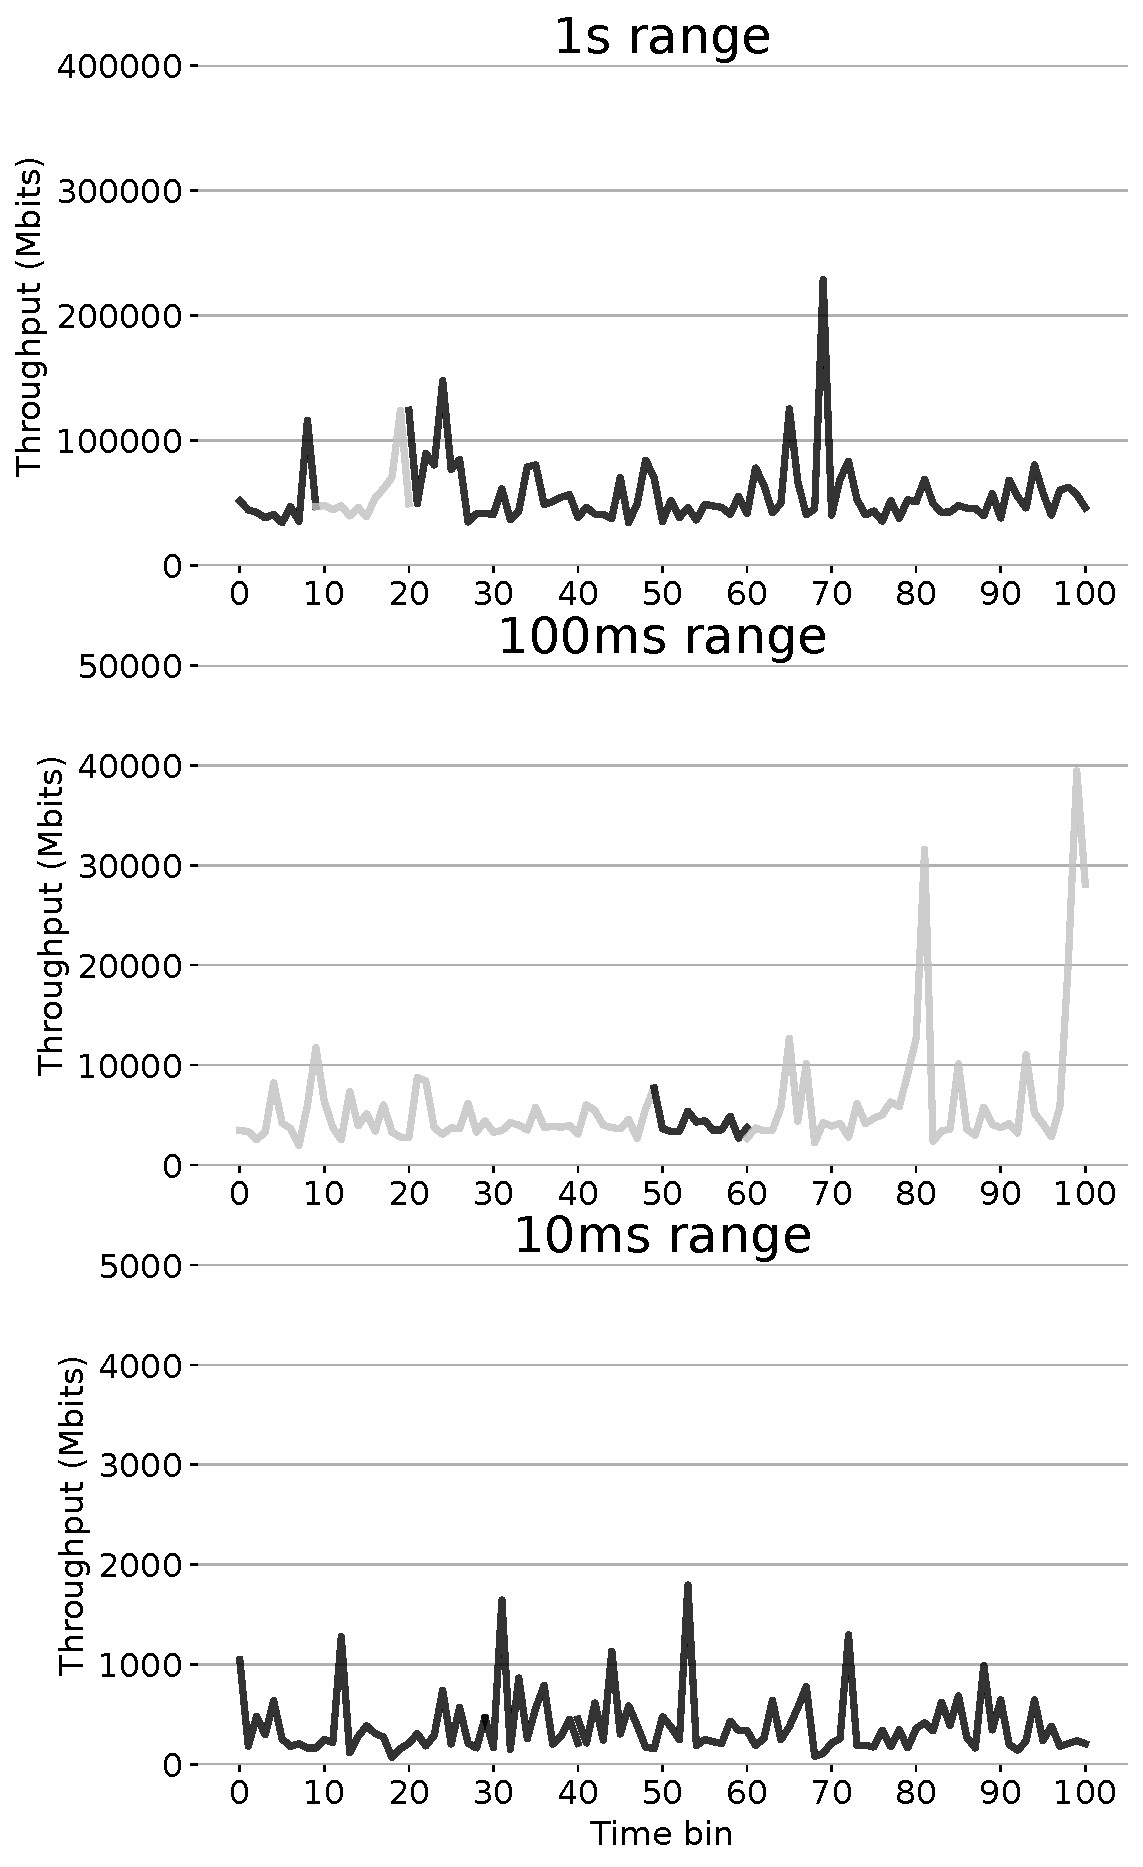
\includegraphics[width=1\linewidth]{figs/self_similarity.pdf}
    \caption{\textbf{Time-series}}
	\label{fig:self-sim}
\end{subfigure}
    \begin{subfigure}[t]{0.33\linewidth}
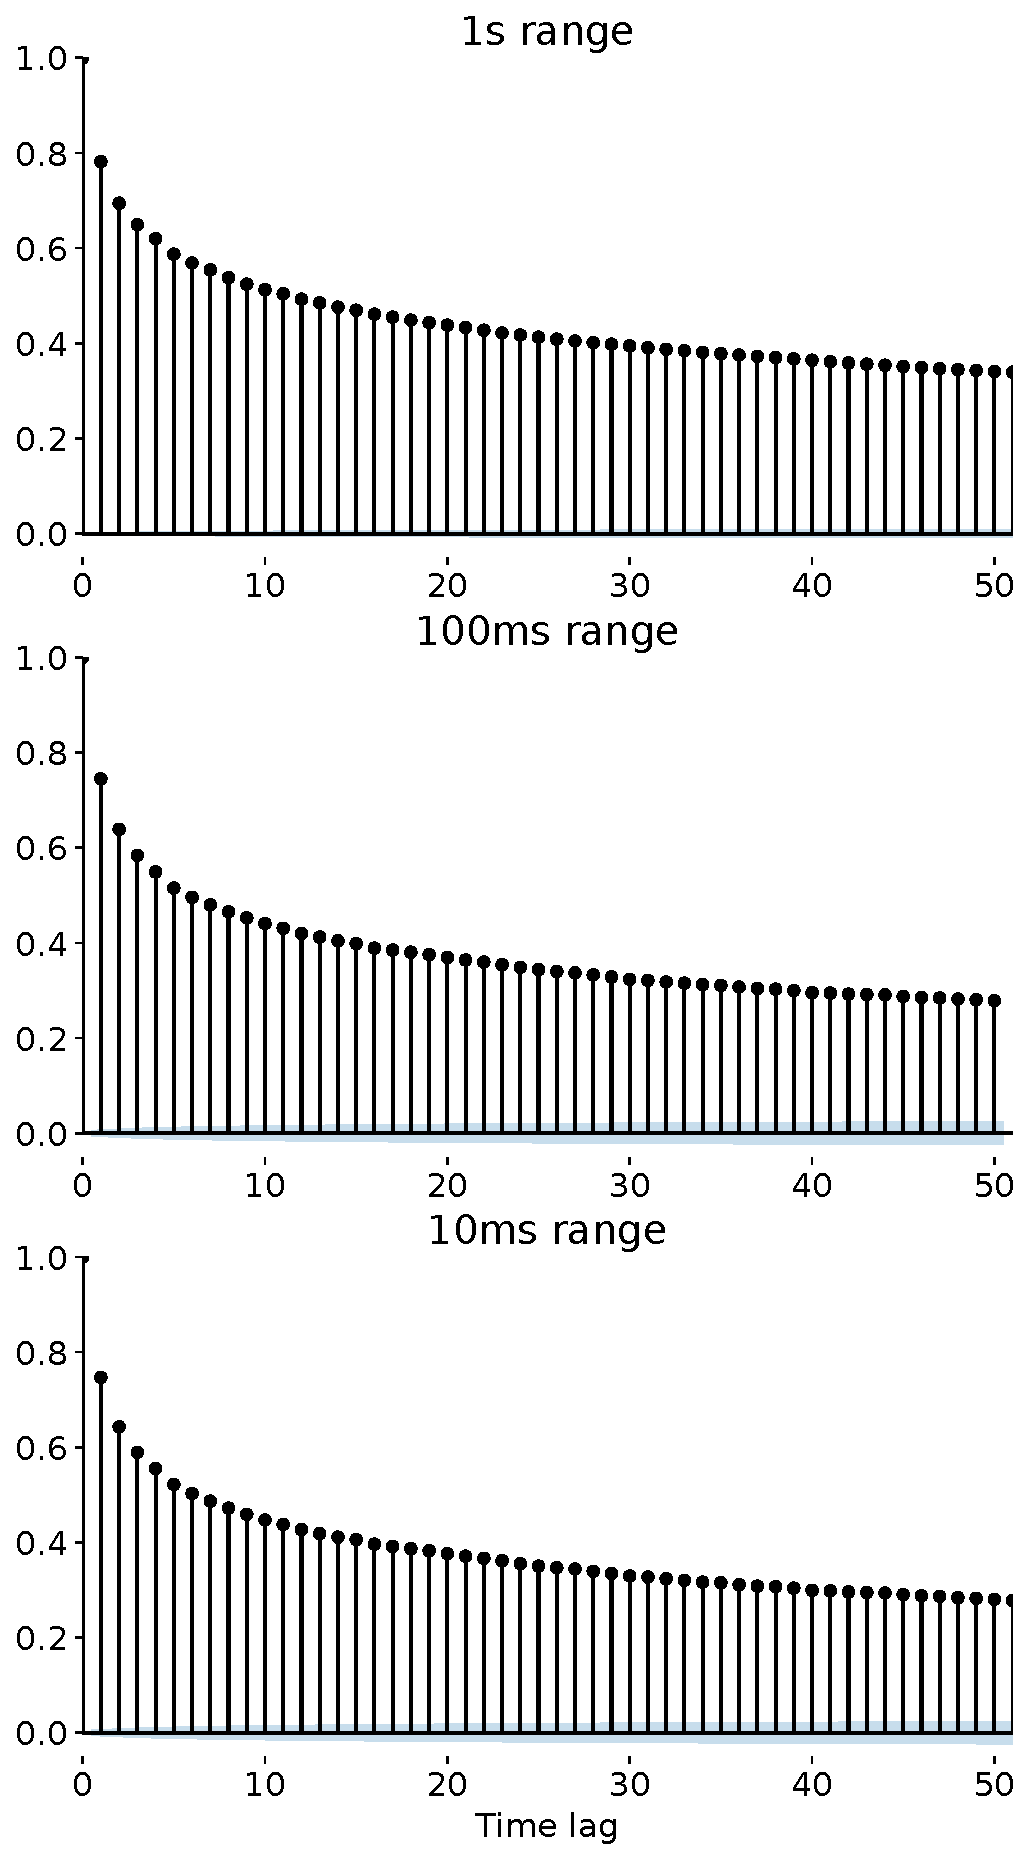
\includegraphics[width=1\linewidth]{figs/acf.pdf}
    \caption{\textbf{Auto-correlation}}
	\label{fig:autocor}
\end{subfigure}
 % \vspace{-3mm}
    \caption{\small{A self-similar timeseries with H=0.88.}}

\label{fig:motiv}
 \vspace{-2mm}
\end{figure}

\paragraph{Example:} Figure \ref{fig:self-sim} (the first row) shows a simulated scenario where 32 TCP connections generate a synthetic workload using Pareto flow size distribution with a mean of 4200 kB and $\alpha=1.05$ and exponential arrivals that create 6 Gbps offered load.
We plot the traffic rate (in Mbps) against time where time granularity is 1$s$. A data point is the aggregated traffic volume over a $10 ms$ interval. The second row of the same figure depicts the same traffic series where a randomly selected second interval in the first timeseries (the highlighted segment in the first row) is magnified by a factor of ten, resulting in a granularity of $100 ms$ in the truncated timeseries. The last row similarly rescales a randomly selected slot by 10$\times$. The figures show that this trace is self-similar: when traffic is aggregated over varying timescales, the aggregate traffic pattern remains bursty, regardless of the granularity of the timescale. 
%
This visual scaling is confirmed by the Hurst coefficient, $H=0.88$, and the autocorrelation functions of the trace (Figure \ref{fig:autocor}) that show positive, slow (almost polynomial) decaying, and consistently shaped correlations across various timescales. Slow-decaying ACFs signify long-range dependence in a timeseries.

\paragraph{Practical implications of self-similarity.}
Self-similarity has broad implications on network design and performance, e.g., it is shown to lead to increased delay and loss \cite{filesize, mts_cc, adas1995resource, addie1995fractal, duffield1995large, likhanov1995analysis, norros1994storage}. We next discuss some of the key implications of self-similarity: 

\begin{compactitem}
\item{\textbf{Queueing performance and buffer sizing.} Self-similarity greatly influences queueing performance. From a queueing theory standpoint, the defining characteristic of self-similarity is that the queue length distribution decays much more slowly than short-range-dependent traffic (polynomially vs. exponentially under short-range dependent traffic, e.g., Poisson processes) \cite{mts_cc}. For strongly self-similar traffic, the mean queue length increases with the buffer size \cite{park1997effect}. This implies that  networks with strongly self-similar traffic should deploy small buffers to control the queueing delay. }

\item{\textbf{Throughput and latency trade-off.} Prior work \cite{filesize, park1997effect} shows that jointly provisioning low delay and high throughput is adversely affected by self-similarity.}

\item {\textbf{Traffic prediction and burst countermeasures.} The correlation structures present in self-similar traffic can be detected and exploited to predict future traffic over timescales larger than an RTT \cite{mts_cc}.\footnote{The prediction methods span diverse domains such as regression theory, neural networks, and estimation theory \cite{mts_cc}.} Traffic prediction at long timescales, in turn, is invaluable for designing the appropriate burst countermeasures. For instance, resource provisioning techniques with control loops larger than an RTT (e.g., multi-scale congestion control \cite{mts_cc}, re-routing, and topology rewiring \cite{gemini}) enhance the performance of self-similar traffic.}

\end{compactitem}


\paragraph{Microbursts.} Given their ubiquity and impact, in particular in data centers, microsecond-scale traffic surges, known as \emph{microbursts}  \cite{wild,hpcc,high-resolution}, have been the focus of many recent proposals \cite{conquest,vertigo,acc,swift,bfc,hpcc}.

The intensity of a microburst has often been measured implicitly based on buffer utilization, or in more extreme cases, packet loss. Related work also quantifies microbursts as the number of packets from one flow that occupy a buffer at a time snapshot \cite{radar}, the evolution of switch queue length over time \cite{observation}, an uninterrupted sequence of packets with gaps of smaller than a threshold \cite{bullet}, and/or sequence size of larger than a threshold \cite{bs}.
Using metrics that are independent of network queues allows us to perform universal measurements in the entire network, i.e., both at the hosts and the switches. Yet, measurement systems intending to quantify microbursts can leverage all the above definitions to provide a holistic view of burstiness behavior.

From the technical perspective, we define a burst as the cumulative sum of packet bytes whose inter-arrivals are smaller than a threshold $\tau$. Setting the minimum value for $\tau$ initially depends on link speeds and MTUs. For example, in a fully utilized 40 Gbps link with MTU = 1500 bytes, packets arrive 300 ns apart. Therefore, an initial $\tau$ of 2-10$\times$ of this value is small enough to detect microbursts and large enough not to miss consecutive packets from flows. To ensure that $\tau$ is not affected by the network configuration and the internal characteristics of the workloads, we repeat our measurement with a wide range of values for $\tau$.


\section{Approaches to measuring traffic bursts}
\label{sec:valinor-space}
%In order to explore the design space for capturing packet arrivals, it is worthwhile to first review the path of the packets in the network stack.
In this section, we provide a brief background on host networking and present the design space of burst measurement frameworks before discussing Valinor in \S\ref{sec:valinor}.

\begin{figure}
    \centering
    	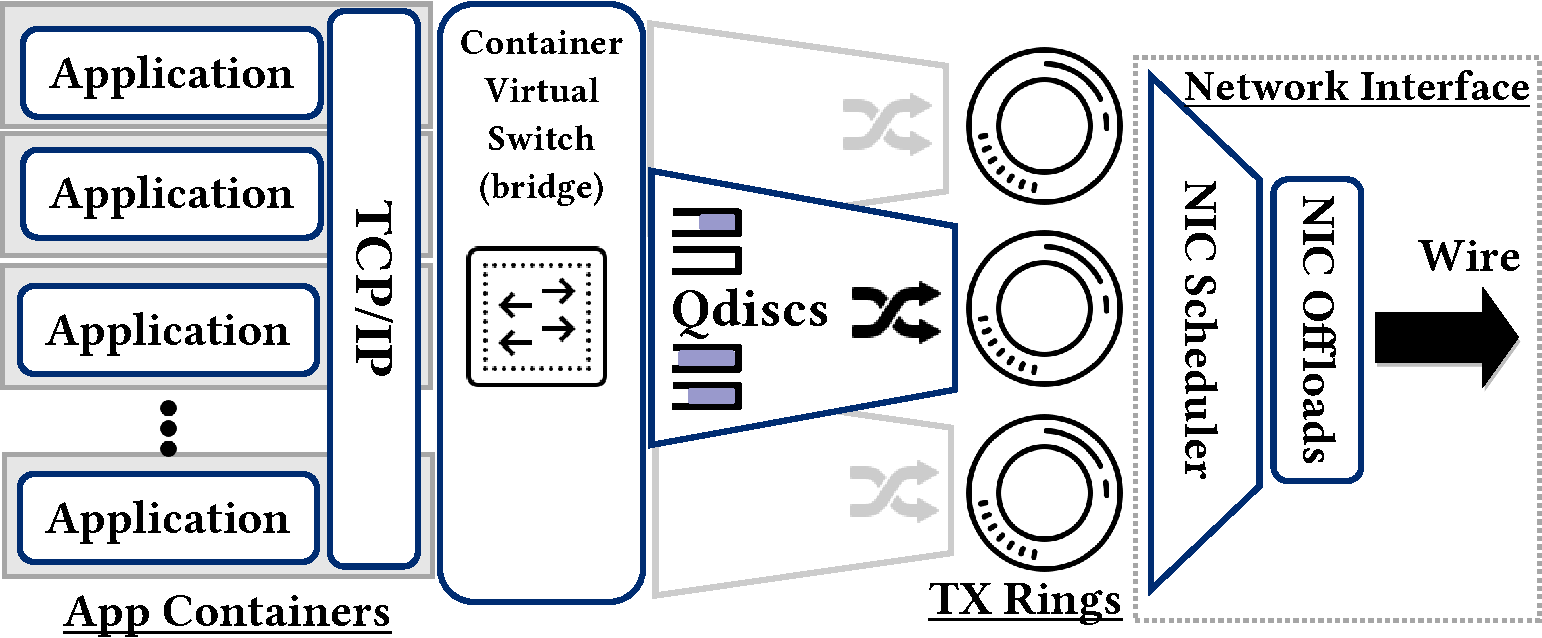
\includegraphics[width=0.80\linewidth]{figs/hostack-crop.pdf}
    	% \vspace{-2mm}
    \caption{\small{Conventional network processing stack architecture in a containerized Linux deployment.}}
    \vspace{-2mm}
	\label{fig:hostack}
	    \vspace{-3mm}
\end{figure}

\subsection{Conventional host networking}
Conventional network stacks consist of various processing layers glued together via several optimization techniques. In Linux, application data is passed to socket interfaces (buffering in the userspace), and then to the transport protocol processing (transport buffers, short queues \cite{tsq}). Transport protocols populate \textit{sk\_buffs},\footnote{\textit{sk\_buff} stands for "Socket buffer" and is used to represent the socket data that eventually is shaped into the packet. \textit{sk\_buffs}, therefore, may contain a single or multiple packets.} a collection of data pointers and  header information. After performing routing, \textit{sk\_buffs} eventually make their way towards interface \textit{qdiscs}, the hierarchical packet schedulers in Linux. \textit{qdiscs} operate in parallel on all CPU cores and forward the scheduled \textit{sk\_buffs} towards driver rings where another layer of buffering is performed before notifying the NIC \cite{titan}. Finally, with the conventional offloading features enabled, the NIC performs scatter/gather \cite{breakfast}, segmentation, checksum, and sends the packets on the wire \cite{overheads}. Figure \ref{fig:hostack} depicts an overview of the packet's path through the network processing pipeline in a Linux host.

% \subsection{Designing a measurement framework: challenges and trade-offs}
% Figure \ref{fig:timestamp} depicts potential means of capturing timestamps to measure traffic burstiness during packet transmission.
% \begin{table*}[t]
% \resizebox{\textwidth}{!}{%

% \begin{tabular}{l|c|c|c|c|c|c|c|c|c}
% \rowcolor[HTML]{dfe9f8} 
% \multicolumn{1}{c|}{Method} & \multicolumn{1}{c|}{Latency}  & \multicolumn{1}{c|}{Throughput}  & \multicolumn{1}{c|}{CPU utilization}    & \multicolumn{1}{c|}{Interference}   & \multicolumn{1}{c|}{Scalability}          & \multicolumn{1}{c|}{Granularity}  & \multicolumn{1}{c|}{Data analysis} & \multicolumn{1}{c|}{Intermediate layer capture} & \multicolumn{1}{c}{Wire traffic capture}  \\ \hline \hline
% % \rowcolor[HTML]{fbe5d6} 
% In-network timestamping  & \cmark & \cmark & \cmark & \cmark & \cmark & Packets & Offline & \xmark & \cmark \\ \hline
% \rowcolor[HTML]{dfe9f8} 
% eBPF timestamping on TX path     & \xmark & \xmark & \xmark & \xmark & \cmark & sk\_buffs & Offline & \cmark & \xmark \\ \hline
% % \rowcolor[HTML]{fbe5d6} 
% Commodity NIC timestamps        & \cmark & \cmark & \xmark & \xmark & \xmark & sk\_buffs & Offline & \cmark & \xmark  \\ \hline
% \rowcolor[HTML]{dfe9f8} 
% Programmable NIC timestamps & \qmark & \qmark & \qmark & \cmark & \cmark & Packets & Offline/Online & \qmark & \qmark \\ 
% \end{tabular}
% }
% \vspace{-3mm}
%   \caption{\small{\textbf{Different approaches to capturing packet arrivals. Checks (\cmark) represent the utility of the proposed solution. Crosses (\xmark) represent the shortcomings, and the question marks (\qmark) demonstrate inconsistency in available features. In-network timestamping provides a zero-overhead and scalable way to monitor traffic burstiness but lacks visibility into host stack intermediate layers. eBPF data planes provide better visibility into qdiscs and transport protocol's traffic shape but suffer from software overheads.}}}
% %   \vspace{-0.8cm}
% \vspace{-5mm}
%   \label{tab:techniques}
% \end{table*}

\subsection{Capturing timestamps}

High-resolution timestamping is essential for burst analysis. Various techniques exist for capturing packet arrivals:
\\
\\
\textbf{NIC timestamps.}
Hardware timestamping is available in all commodity NICs. This feature  is supported by the Linux kernel via ancillary socket data. When a user requests timestamping through a socket option, the transmission timestamps are generated in the hardware before sending the packet on the wire and are eventually sent to the source socket. Therefore, the application is responsible for polling the error queue and reading the timestamps.
Hardware timestamping supports most TCP and UDP connections, however, it suffers from two main shortcomings.
First, if the operating system fails to poll the timestamp registers of the NIC in time, e.g., in higher packet rates, the timestamp will be overwritten by that of the next packet.
Plus, modifying the network application to receive timestamps may impact the application's workload pattern, and thus must be performed with extra care.
\\
\textbf{Modifying networking stack software.}
To study realistic network traffic with higher arrival rates, hardware timestamping is not ideal due to the need to change the application internals and high overheads. An alternative solution is to directly capture the timestamps closer to the packet processing, e.g., the NIC driver, and either add the timestamps to the packet payload or re-route them to the userspace. Alas, accessing and modifying the packet data requires offloading features such as scatter-gather IO and Segmentation Offloading to be turned off. Additionally, timestamps that are at \textit{sk\_buff} granularity may not imitate the inter-packet gaps on the wire due to the intervention of lower layers.
\\
\\
\textbf{eBPF hooks.}
eBPF offers a series of hooks inside the Linux kernel and the NIC driver that allows fast execution of arbitrary data plane logic. An eBPF program consists of a data plane and a control-plane code targeting a specific hook on the RX or TX path (XDP hook in the receive path of NIC driver and traffic control (\textit{tc}) hook on the TX path of the qdisc subsystem are two examples). eBPF \textit{tc} programs are registered to the kernel using the \textit{tc} command and are executed inside a lightweight RISC virtual machine. eBPF also provides fast data structures that enable shared state between the kernel and the userspace. This allows us to perform burst measurements offline with any workload configuration without modifying the kernel source or packet payloads.

While eBPF relieves us from directly modifying the packet processing code in the kernel, it presents two shortcomings. First, eBPF, similar to the previous solution, works at \textit{sk\_buff} granularity since packet segmentation is almost always offloaded to the NIC. Therefore, the eBPF framework can only measure the gaps between larger chunks of data, not packets. Additionally, our measurements show that each eBPF invocation incurs  up to 1 $\mu$s of delay, mostly due to memory accesses. While this overhead may be acceptable at the \textit{sk\_buff} granularity, the framework will lose its visibility into nanosecond-scale events. Ultimately, eBPF provides a convenient solution to plug into the network data path with minor interference. Making it a viable burstiness probing point on the egress path. We present the design and implementation of the Valinor eBPF framework, Valinor-H, in \S\ref{sec:host}.
\\
\\
\textbf{Timestamping in the switch data-plane.}
A holistic method to capture the behavior of all host networking components (including the NIC) is to perform measurements immediately after transmitting the packets on the wire, i.e., at the first network hop. Fortunately, the rise of programmable switch architectures with high-resolution timestamping enables capturing packet arrival timestamps and sending this data off the critical communication path for offline processing.
This further ensures zero interference with the ongoing communication and the ability to track the entire egress host networking components. We describe the design of our in-network measurement system, Valinor-N, in \S\ref{sec:innetwork}. 
\\
\\
% Table \ref{tab:techniques} summarizes the advantages and disadvantages of using the above techniques for timestamping. eBPF timestamping does not require any modifications to the kernel or the application--unlike commodity NIC timestamps--but suffers from slight performance degradation due to the additional imposed latency. The added latency is further amortized when breaking a large sk\_buffs to smaller MTUs. In-network timestamping allows fast accurate acquisition of telemetry data that is sent to offline servers for processing.
\textbf{Programmable NICs} share many of the strengths of in-network measurements (e.g., timestamping close to the wire, low overhead, and no interference) but do not provide visibility into in-network queue occupancies. Plus, our experience with commodity DPUs \cite{dpu} shows inconsistencies in the capabilities of existing devices. General-purpose SoC NICs \cite{dpu} are either bound to their slow ARM CPUs or do not offer per-packet timestamping capabilities on their fast path. Due to these practical issues as well as the greater visibility that in-network measurements offer, alongside its host module, Valinor currently leverages programmable networks for capturing bursts on the wire.

% Finally, with the rise of programmable network interfaces, we envision that they can eventually embrace in-host traffic measurement frameworks. Our initial experience in trying to implement a traffic measurement framework in commodity DPUs \cite{dpu} reveals that existing devices are not consistent in their capabilities. General-purpose SoC NICs \cite{dpu} are either bound to their slow ARM CPUs or do not offer per-packet timestamping capabilities on their fast path. On the other hand, a full design and implementation of a traffic measurement framework on an FPGA-based NIC is beyond the scope of this study, yet a viable future direction that can combine the visibility of in-network frameworks with the scalability of in-host alternatives.

\section{Valinor measurement framework}
\label{sec:valinor}

For designing Valinor, we have three goals in mind:
\begin{compactenum}
    \item Offering visibility into the host networking traffic, as well as the shape of the traffic on the wire.
    \item Offering high-resolution timestamping of packet arrivals in line with the increasing link bandwidths and faster packet processing pipelines.
    \item Providing insights on traffic shape and burstiness at different scales and time ranges.
\end{compactenum}

We design and implement Valinor, a measurement framework that consists of two main timestamping prongs to study packet arrivals from the host and network vantage points.
First, we design Valinor-H to study the host's view of its egress traffic by choosing \textit{tc} eBPF hooks. For capturing the external picture of traffic burstiness, we design Valinor-N, a timestamping module for programmable fabric.

\subsection{Valinor-H: burst measurement in hosts}
\label{sec:host}
% Capturing packet departures in the host network stack requires direct visibility into the kernel. eBPF offers a series of hooks inside the Linux kernel and the NIC driver that allows fast execution of arbitrary data plane logic. An eBPF program consists of a data-plane and a control-plane code targeting a specific hook on the RX or TX path (XDP hook in the receive path of the NIC driver and \textit{tc} hook on the TX path of the qdisc subsystem are two examples). We target the \textit{tc} hook and design Valinor-H data plane to capture \textit{sk\_buff} metadata and store them in shared kernel buffers. The corresponding control plane reads and stores the timestamp records for offline analysis.
Valinor-H offers visibility into the impact of the software stack on traffic, immediately before the traffic is passed to the NIC. The insight into the characteristics of the traffic entering the hardware can help the design of the functions offloaded to the NIC. This becomes increasingly important as more and more functions migrate to the NIC, driven by the dire need to reduce software overhead.\footnote{As network speeds increase at a faster pace than CPU speeds, software overhead is increasingly the performance bottleneck \cite{homa-impl}. This has motivated the offloading of various functions such as segmentation, serialization, scheduling, and even transport protocol processing to the NIC \cite{programmable-transport,loom,breakfast}.}

\begin{figure}
    \centering
    	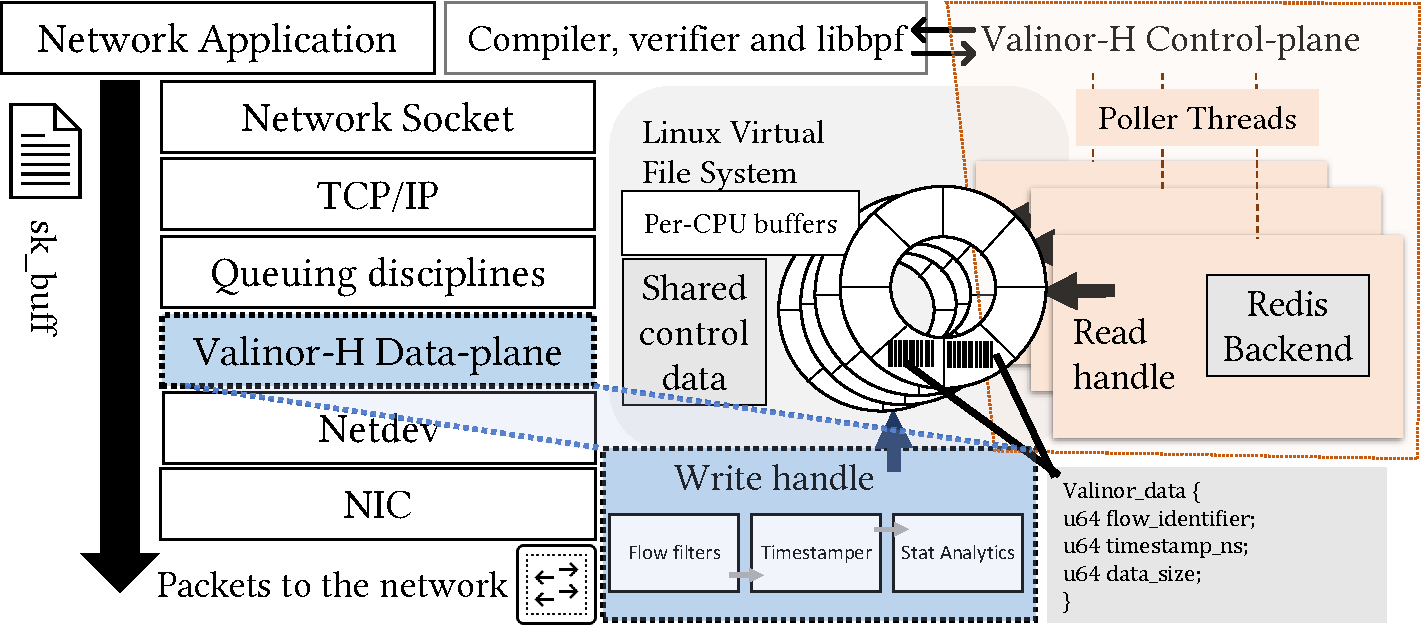
\includegraphics[width=0.85\linewidth]{figs/ebpf-crop.pdf}
      % \vspace{-4mm}
    \caption{\small{Valinor-H consists of an eBPF-based data plane and a control plane, communicating via lock-free ring buffers.}}
	\label{fig:bpf}
 % \vspace{-3mm}
\end{figure}

% \subsubsection{Framework design and implementation}
Figure \ref{fig:bpf} presents the design of our eBPF framework. Our framework consists of two separate programs. The data plane program follows a strict set of C-like instructions that are executed at the \textit{tc} qdisc, every time a \textit{sk\_buff} arrives. We design circular buffers capable of storing up to $2^{16}$ arbitrary data entries shared with the control plane. Then, the \textit{write handle} determines the correct location for adding new timestamp entries and updates the data structure. In the control plane, we initialize the data plane and the circular buffer and start polling the buffer for new data. The data entries carry the \textit{sk\_buff} lengths as well as the flow hash and protocol header information. The \textit{read handle}, retrieves the timestamp entries one by one and hands them to the Redis workers for persistent storage.

One challenge that arises when using a shared data structure is synchronization between the data plane and the control plane. This scenario generally needs locking mechanisms to prevent a race condition, however, the nature of the timestamping data, being strictly increasing, lifts this heavy burden. Therefore, in the control plane, Valinor-H only reads and increments its write handle if the timestamp value is larger than the previous value read.
Another synchronization issue arises when multiple CPUs attempt to store packet metadata in the shared memory. Luckily, eBPF offers per-CPU structures to prevent race conditions in the data plane. The Valinor-H control plane uses separate threads to read from per-CPU buffers simultaneously.

With the in-host measurement framework, network operators can verify the operation of higher-level network processing layers on the transmission path of the sender hosts. Valinor-H, at this stage, can capture the ingress traffic into the NIC which includes the traffic egress from qdiscs, the transport layer, and the applications. To capture the traffic behavior in the core of the network, and on a per-packet granularity, we introduce Valinor-N in the following section.


\subsection{Valinor-N: in-network burst measurement}
\label{sec:innetwork}


Software-based measurements in the host stack are bound to the coarse-grained \textit{sk\_buff} arrivals and are implemented before NIC functions (i.e., ring schedulers and segmentation offloads). Hence, the captured traffic behavior might not match that of the wire. To fill this gap, we introduce the in-network variant of Valinor based on programmable switch data planes.
Valinor-N consists of three pieces: 1) the switch component, 2) the collector data plane, and 3) the analysis component. Valinor-N is able to I) capture per-packet arrival timestamps with zero overhead outside the critical path, II) collect and store timestamp entries arriving at line rate, and III) perform various analyses on timestamp data to provide an in-depth image of the traffic burstiness at different scales. 
\\
\\
\textbf{Valinor Switch.} The switch data plane program uses \textit{mirroring} and \textit{timestamping} functionalities available in the PISA architecture. For every packet that matches user-defined flow filters, Valinor-N appends the arrival timestamp, queuing delay, and the size of the original packet along with its layer l-4 header information to a special IP packet with a pre-defined Valinor header. The packet is then sent to a collector server. The server machine, deployed outside the critical path of the communication between traffic endpoints, aggregates the timestamp information and performs the offline analysis.
\\
\\
\textbf{Timestamp collection.} The collector machine features a userspace packet processing framework based on DPDK that parses the arrived packets and stores the timestamp information along with flow metadata into an in-memory Redis \cite{redis} instance. Analysis of the timestamp data is then performed by querying the data store.
Receiving timestamp packets at line rate and storing them in persistent storage poses several scalability challenges to the design of the collector component. 
To ensure that software can drain NIC buffers at line rate, we designate multiple worker threads to read and process the incoming packets. After parsing timestamp headers, the worker threads extract the timestamp data and send them to additional worker threads that are responsible for communicating with Redis. The stored metadata is then retrieved by the analysis framework to perform  burst analysis using timestamps.

Valinor-N's Redis workers issue batched commands during idle periods to minimize interference with packet processing workers. We use Redis sorted sets to store timestamp entries sorted by arrival times since the packets that arrive at the collector may have a different order from the packets that arrive at the Valinor-N switch data plane. 
We use 1G \textit{hugepages} and large memory pools to ensure that timestamp packets are not dropped at higher rates (Up to 40~Gbps in our testbed).
\\
\\
\textbf{Offline timestamp processing.} The last piece of Valinor's design is the offline timestamp analysis framework that queries the Redis data structures and performs analysis on timestamp data. Our framework is able to report various statistics on traffic burstiness by measuring the packet inter-arrivals. For example, in the next section, we report our findings on the scaling behavior, caused by various packet processing components in the sender machine. We report actual burst sizes in bytes, inter-arrival distributions, queueing delays, and various burstiness time series analyses. We implement the offline processing framework in Python.


% \begin{figure}[t]
% \centering
% \begin{subfigure}[t]{0.52\linewidth}
%     \centering
%     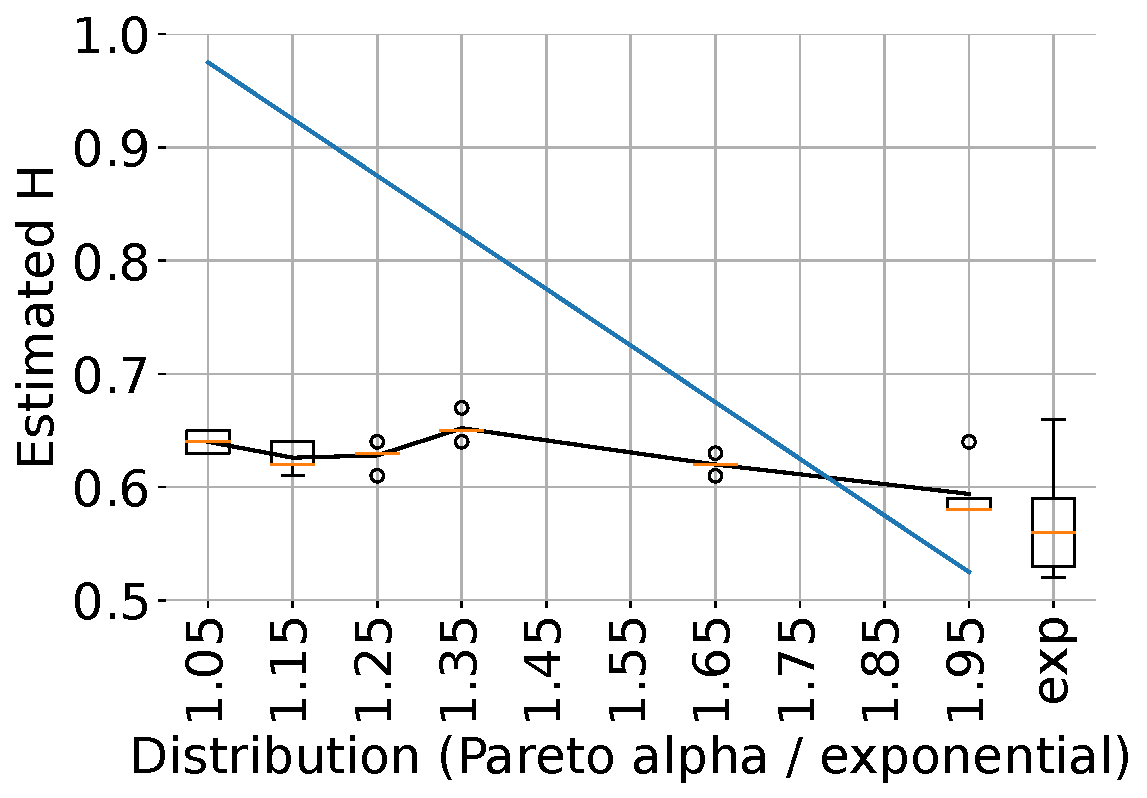
\includegraphics[width=1\linewidth]{figs/filehurst_ebpf_testbed.pdf}
%     \caption{\small{\textbf{Synthetic-Hurst exponents}}}
% 	\label{fig:fhurst-ebpf}
% \end{subfigure}
% \begin{subfigure}[t]{0.46\linewidth}
%     \centering
%     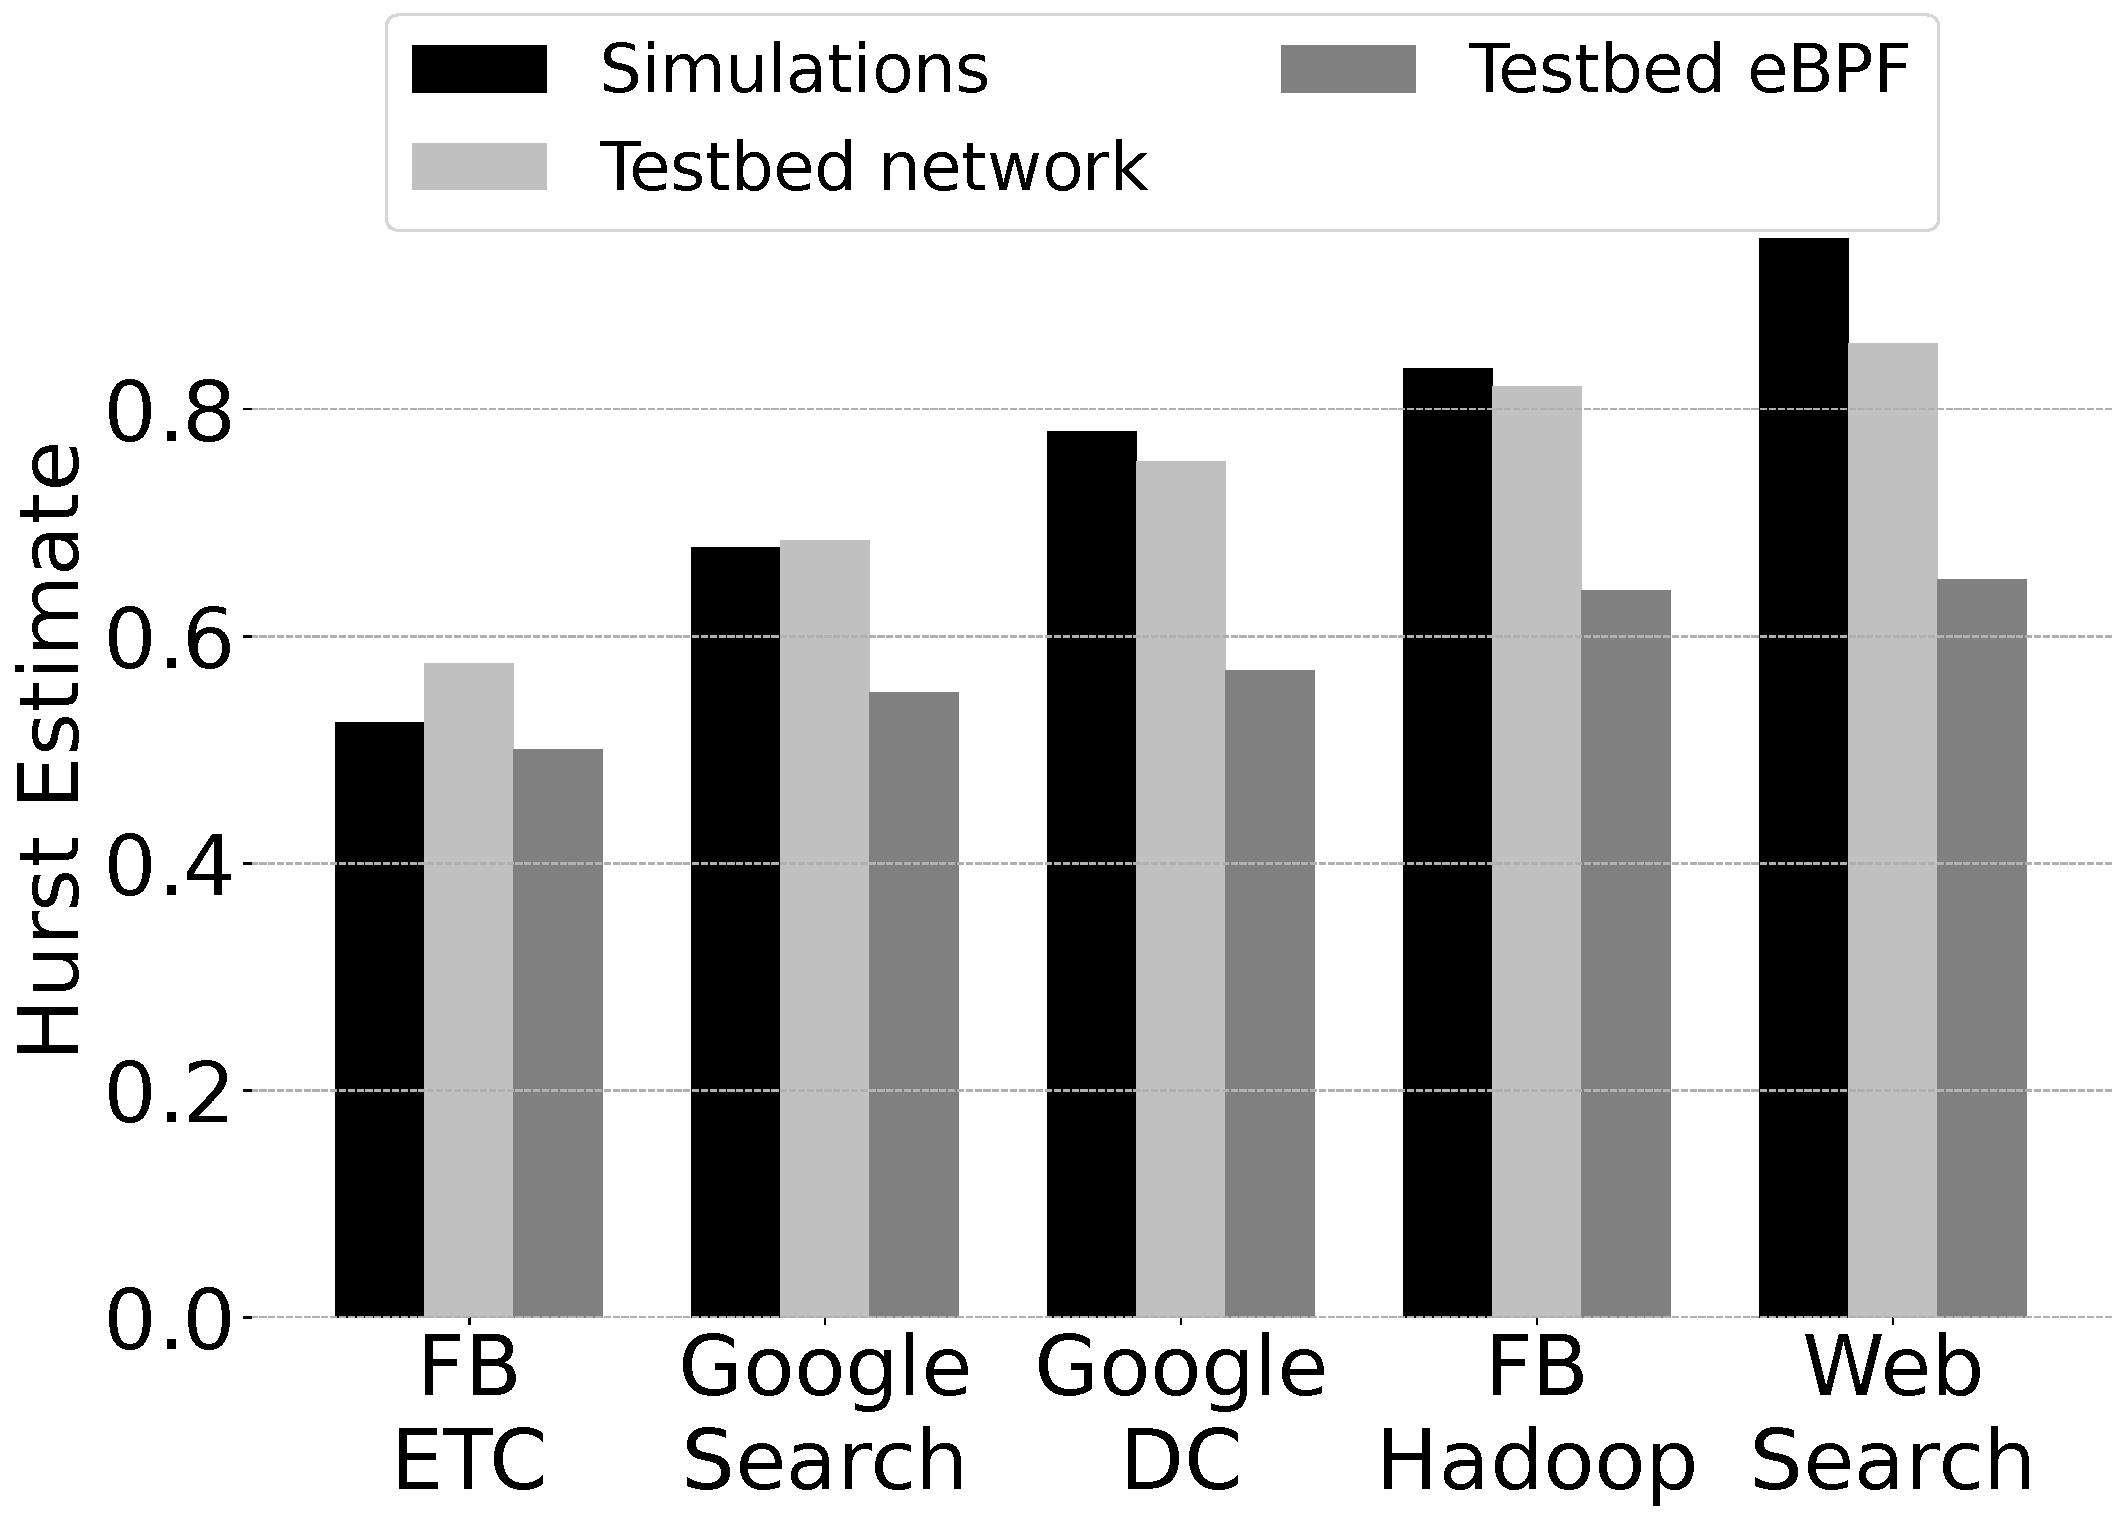
\includegraphics[width=1\linewidth]{figs/w_ebpf_hurst_bar.pdf}
%     \caption{\small{\textbf{Trace-Hurst exponents}}}
% 	\label{fig:whurst-ebpf}
% \end{subfigure}
% \begin{subfigure}[t]{0.49\linewidth}
%     \centering
%     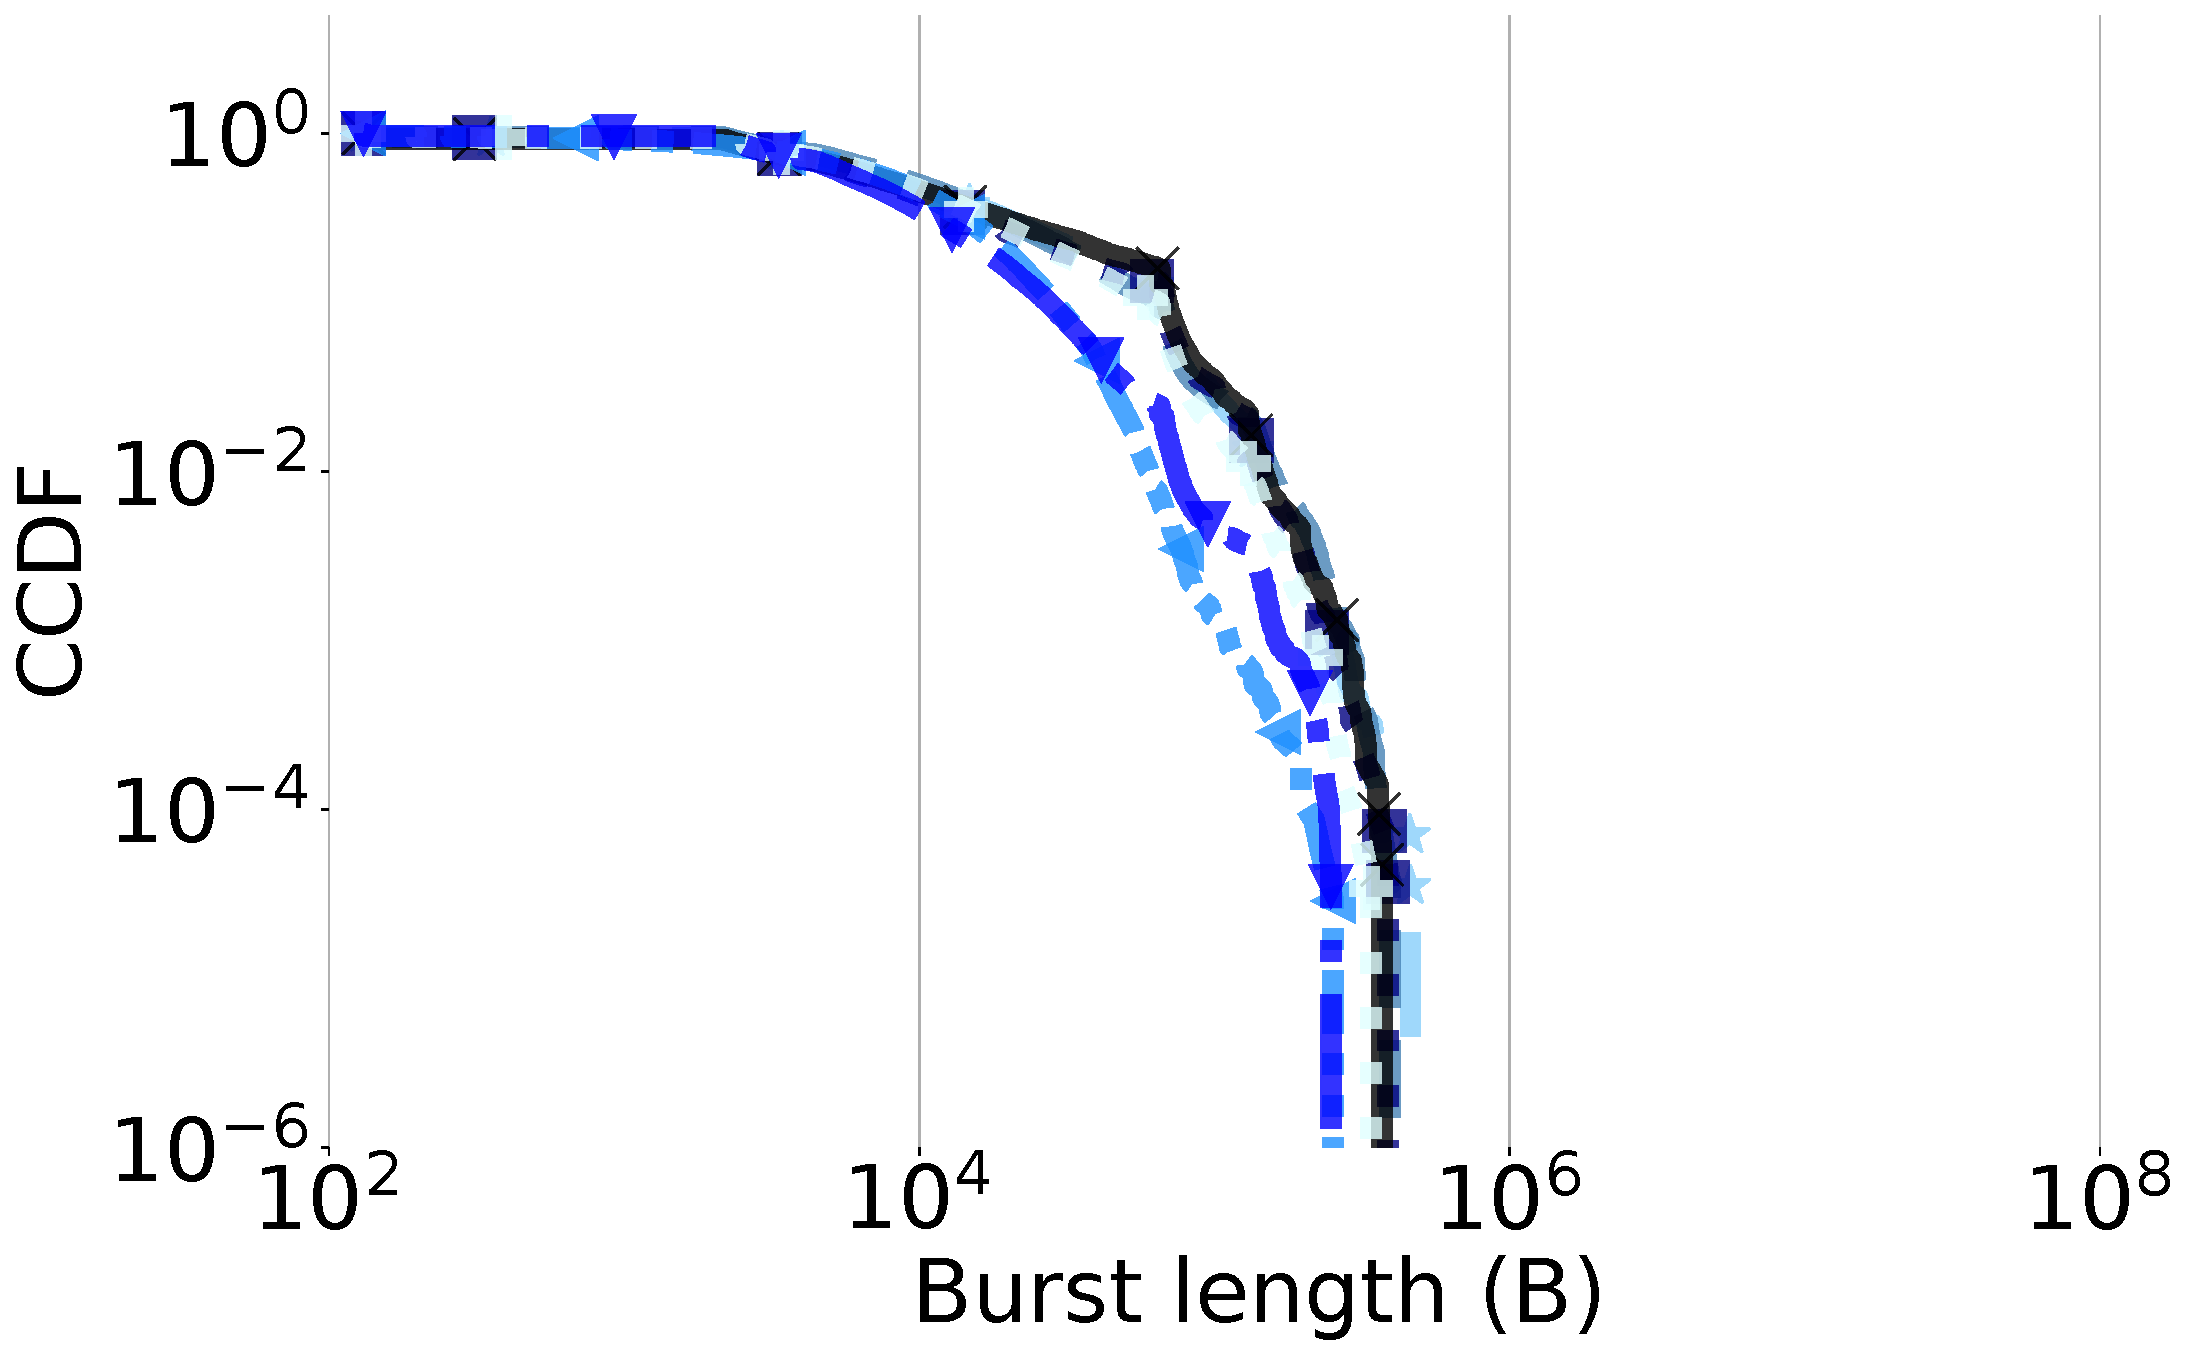
\includegraphics[width=1\linewidth]{figs/fileccdf_ebpf_testbed.pdf}
%     \caption{\small{\textbf{Synthetic-burst length CCDF}}}
% 	\label{fig:fccdf-ebpf}
% \end{subfigure}
% \begin{subfigure}[t]{0.49\linewidth}
%     \centering
%     	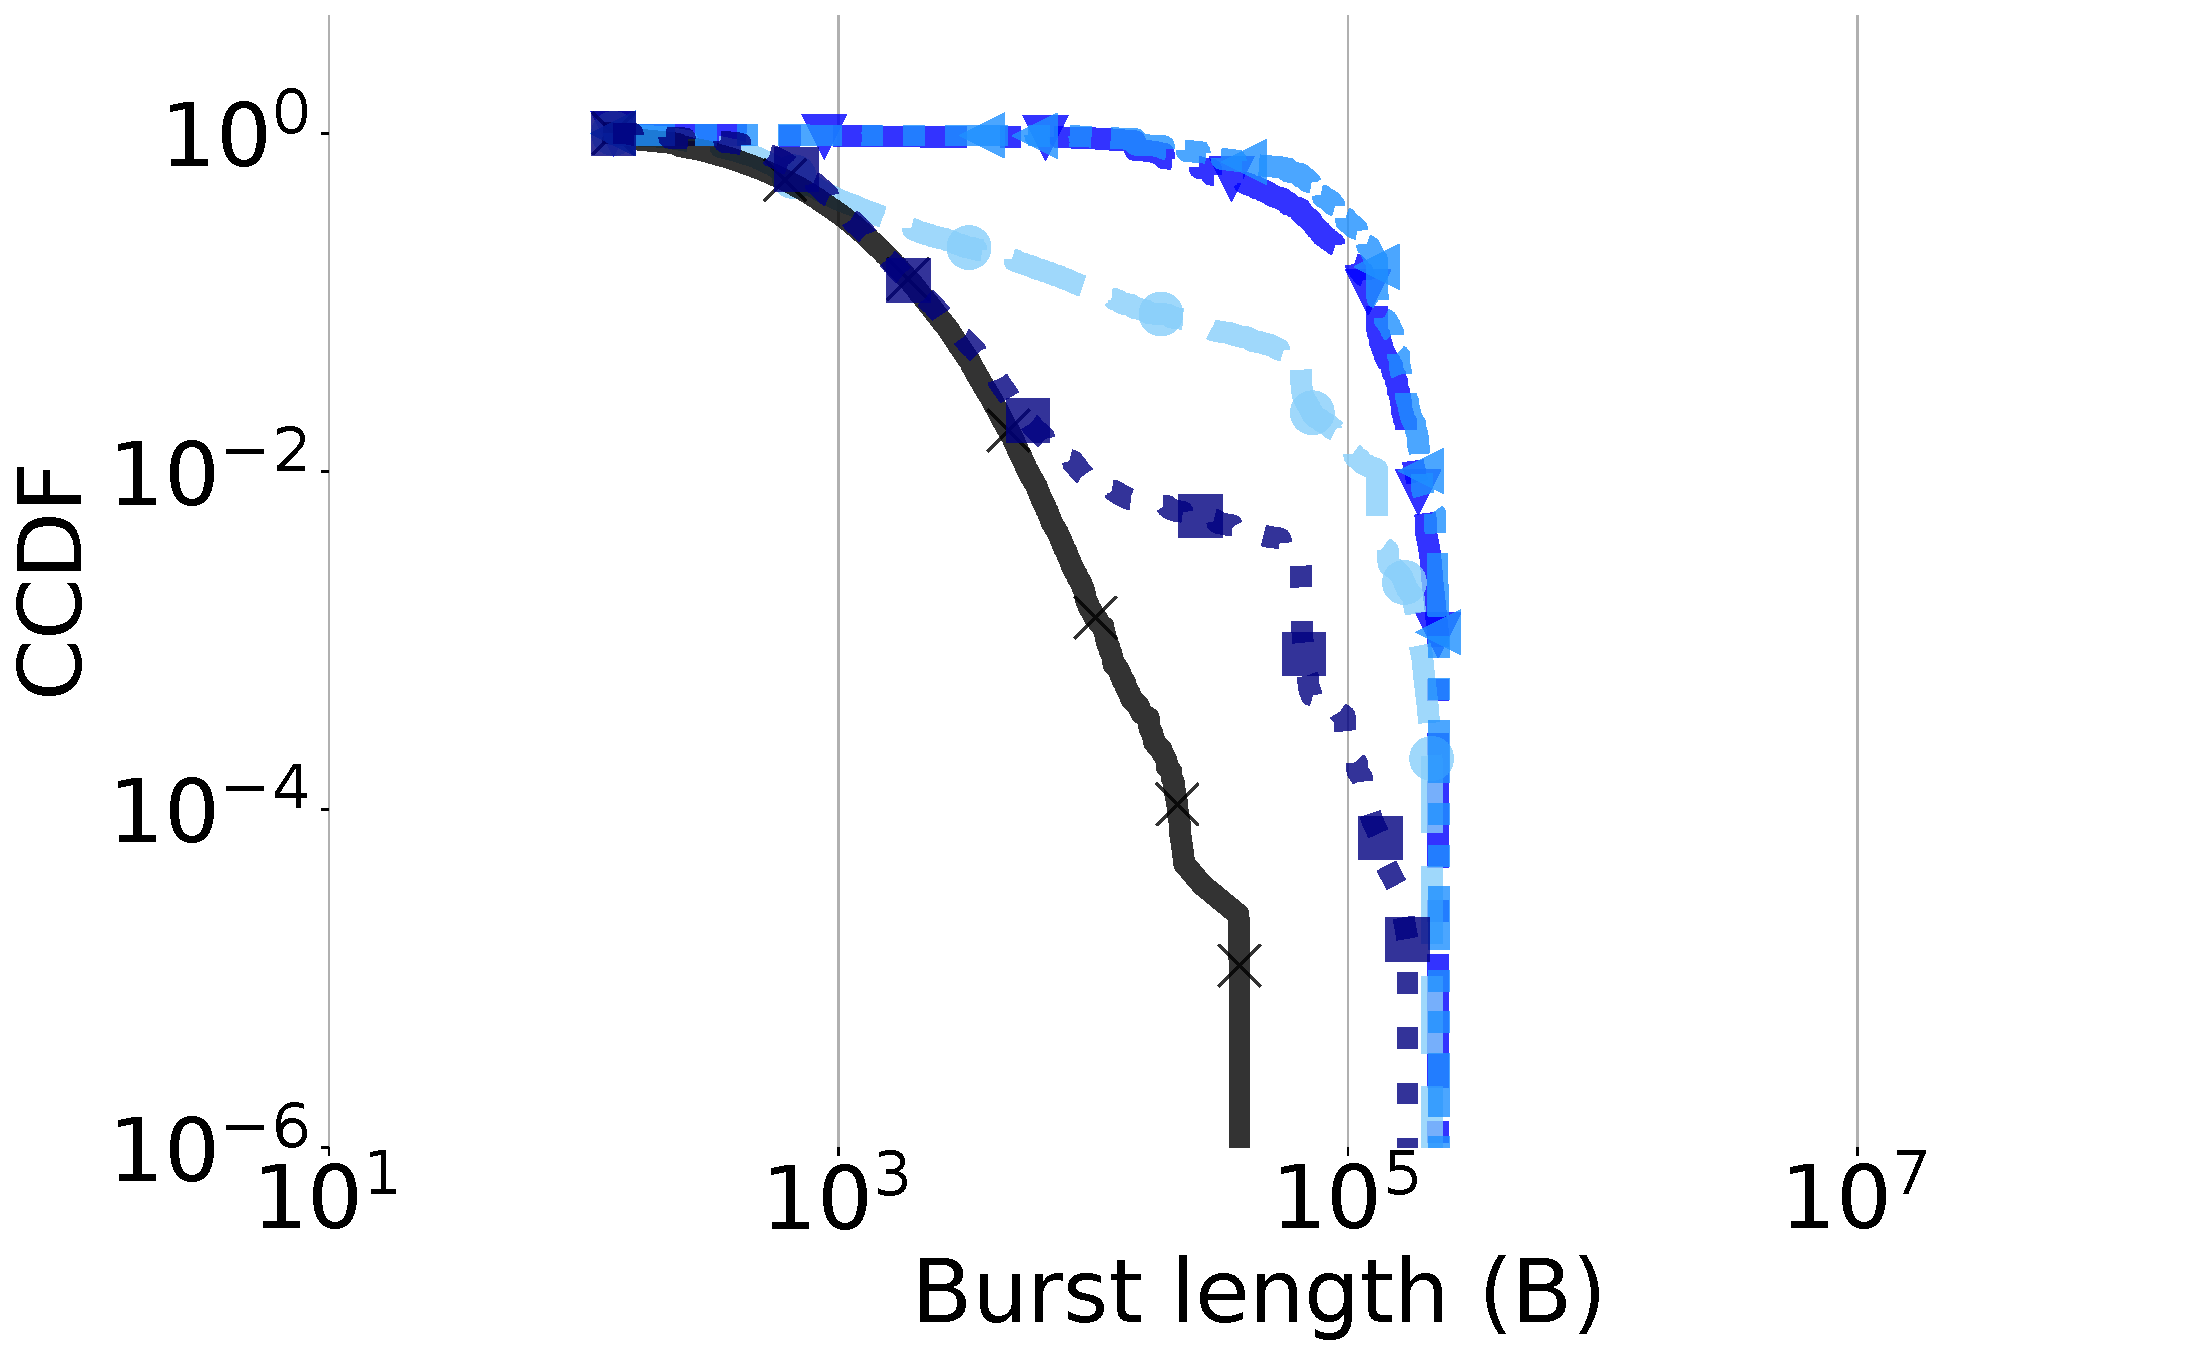
\includegraphics[width=1\linewidth]{figs/wccdf_ebpf_testbed.pdf}
%     \caption{\small{\textbf{Trace-burst length CCDF}}}
% 	\label{fig:fwccdf-ebpf}
% \end{subfigure}
%     \caption{\textbf{\small{\erfan{Repeating synthetic and trace experiments with eBPF framework. Because of the coarser-grained measurements and being placed behind the NIC functions, Valinor-H presents a smoother trend for burstiness compared to Valinor-N. However, Valinor-H is still able to show a relatively accurate picture of the expected traffic burstiness within the host machine.}}}}
% 	\label{fig:ebpf}
% \end{figure}

We deploy Valinor to analyze the burstiness of various workloads and configurations.
%We perform simulations and testbed experiments using the above implementation of Valinor. 
Our results show:
\begin{compactitem}
    % \item \st{Flow-based packet scheduling can have a considerable  impact on blunting microbursts for egress traffic.}\soudeh{Only true for SQ, no offloading (unrealistic).}
    \item Host networking, largely overlooked in prior self-similarity studies, plays a major role in forming and suppressing bursts.
    %Unlike previous conceptions about directly attributing the sources of burstiness to the workload and applications, host networking elements play a key role in reshaping the original workload. 
    
    \item Lower layers of the network processing stack (such as segmentation offloading and NIC scheduling) compromise the effectiveness of software-based traffic shaping and active queue management solutions.
    
    \item Software pacing has major limitations. For workloads with a mixture of short and large flows, lower layers of the network processing stack mask the impact of software-based traffic pacing. For workloads with very short flows, software pacing can blunt bursts but leads to a major increase in RTT and significant throughput reduction. 
    % \st{Software pacing presents inconsistent burstiness behavior towards workloads with different size distributions. }
    
    \item NIC driver buffer sizing and process scheduling can reshape bursts.
\end{compactitem}


\section{Findings}
\label{sec:valinor-findings}
\begin{figure}[t]
    \centering
    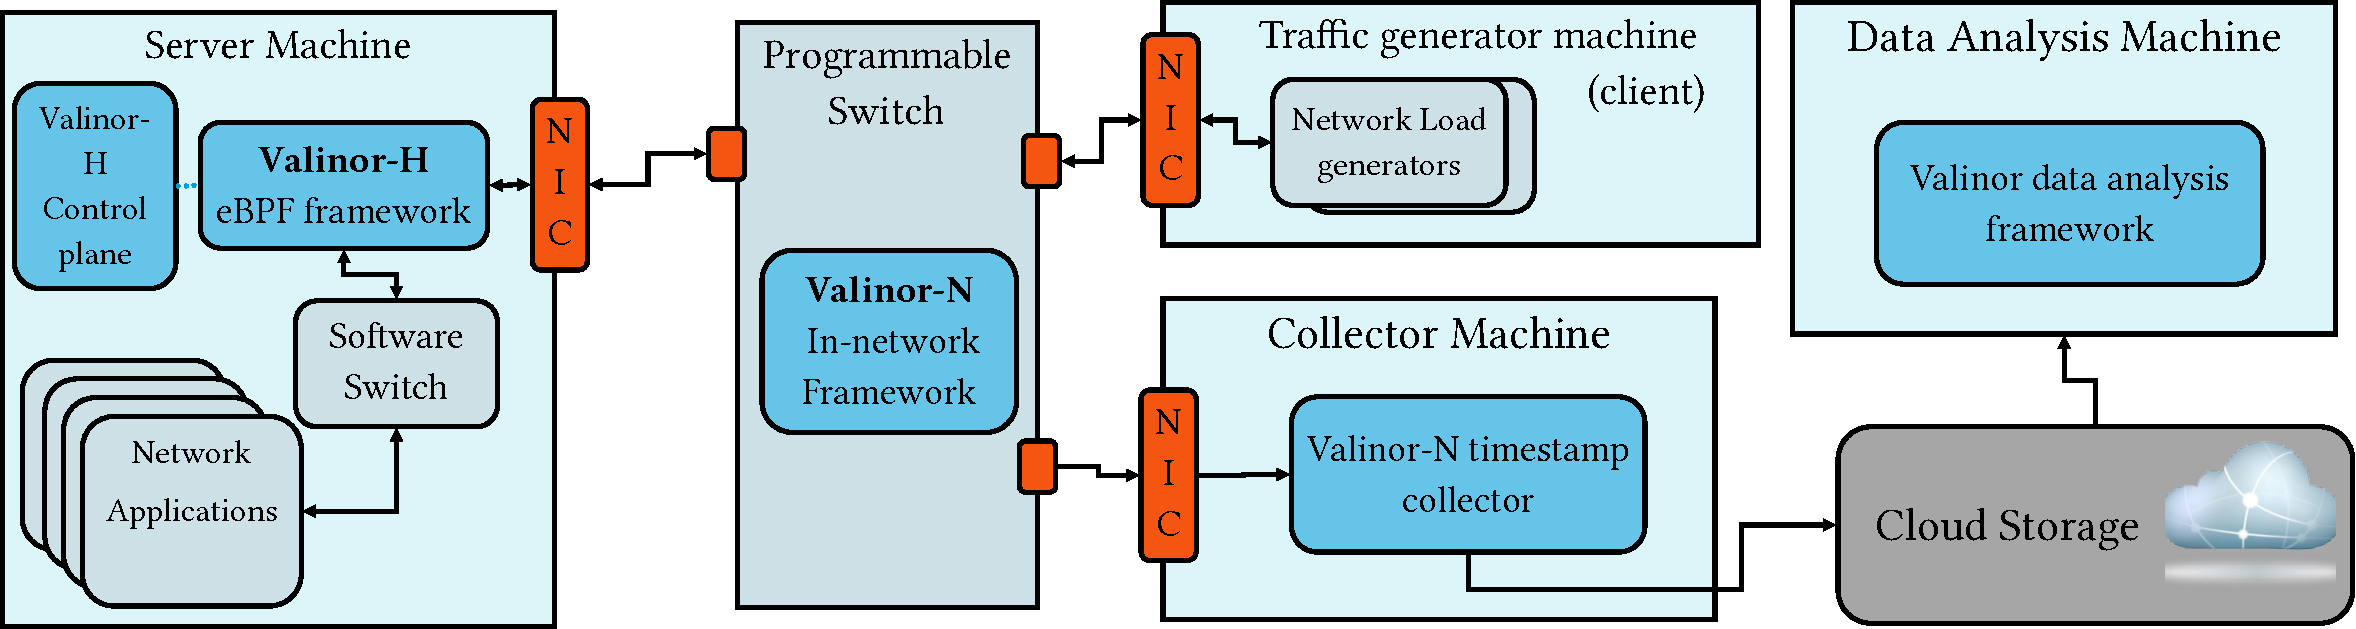
\includegraphics[width=0.9\linewidth]{figs/setup-crop.pdf}
     \vspace{-3mm}
    \caption{\small{Valinor framework deployment overview.}}
	\label{fig:setup}
 \vspace{-2mm}
\end{figure}
% \begin{subfigure}[t]{0.9\linewidth}
%     \centering
%     	\includegraphics[width=0.85\linewidth]{figs/21-2_summary_21_0.png}
%     \caption{\small{Burst behavior of Linux queueing disciplines in the presense of offloading.}}
% 	\label{fig:qdisc_tso}
% 	\end{subfigure}


% \begin{figure}
% \centering
%     	\includegraphics[width=1\linewidth]{figs/qdisc2.pdf}
%     \caption{\small{Impact of per-flow deficits in fq qdisc on traffic burstiness. \erfan{FINALIZED}}}
% 	\label{fig:qdisc_quantum}
% \end{figure}


\paragraph{Experiment setup.}
% We deploy Docker containers hosting applications that resemble widely deployed workloads in data centers. We deploy Memcached for key-value, an in-house restful HTTP server for Web, and Iperf3 containers for throughput heavy workloads. All containers are connected via an OVS \cite{ovs} virtual bridge to the external port. We generate Cache and web workloads using our modified version of Mutilate, based on Facebook's CDF distributions \cite{social}. Our testbed consists of three servers with 1x Intel Xeon  E5-2620 v4 processors, 64 GB of memory and Intel XL710 40G RNICs. We connect the servers via a Wedge Tofino switch augmented with Valinor's timestamping framework. The collector machine features Valinor userspace dataplane based on DPDK v20. We disable idle-states on all servers and set the frequency governor to \textit{performance} to minimize the interference of power-saving features on networking performance.
% Finally, we store the redis data dumps in Azure SMB data shares and use a Cloudlab \cite{cloudlab} server to process the timestamp data.
Figure \ref{fig:setup} demonstrates how Valinor framework components come together in a basic deployment.
For evaluating Valinor, we use a wide range of workload distributions. We deploy Iperf instances alongside Homa's open-source load generator \cite{homa} inside Linux containers and configure the workload generators to simulate different trace-driven workload patterns including Facebook's ETC, Google search, aggregated Google data center, DCTCP's web search, and Facebook's intra-cluster and intra-rack Hadoop traces \cite{social,homa,fb-workload,dctcp}. Unless stated otherwise, all application containers are connected via an \textit{OVS} \cite{ovs} virtual bridge to the external interface.
% For more realistic traces, we preload Memcached \cite{memcached} according to publicly available data center flow size distributions and use a modified version of Mutilate to generate requests using public inter-arrival distributions \cite{social}.
Our testbed consists of servers featuring Intel Xeon  E5-2620 v4 processors, 64 GB of memory, and Intel XL710 40G NICs. We connect the servers via a Wedge-100 Tofino switch running Valinor-N timestamping framework. We deploy Valinor-H on Linux kernel 5.17 with the latest version of \textit{libbpf} and \textit{iproute2} installed. The collector machine features Valinor's userspace data plane based on \textit{DPDK} v20. We disable idle states on all servers and set the frequency governor to \textit{performance} to minimize the interference of power-saving features on networking performance.
The default settings for the evaluated components are summarized in Table \ref{tab:ranges}.

Finally, to calculate microburst lengths, since we use 40Gbps links, we set the burst inter-arrival threshold to 500ns for the presented results (see \S\ref{sec:valinor-background}). Valinor also computes microburst lengths for other threshold settings (ranging from 5ns to 10$\mu$s). 
While the threshold setting impacts the size and quantity of observed bursts, we did not notice any difference in relative burstiness when comparing multiple cases.
We have released Valinor's sources and artifacts as open-source software.\footnote{\url{https://hopnets.github.io/valinor}}
% Finally, we store the Redis data dumps in Azure SMB data shares and use a Cloudlab \cite{cloudlab} server to process the timestamp data

% \subsection{Comparing the burstiness of three different workloads.}
% We run \textit{Iperf3}, \textit{Memcached}, and \textit{HTTP} workloads and generate load using \textit{Iperf3 client}, and \textit{Mutilate}, respectively. Figure \ref{fig:three_workloads} presents the difference in the burstiness of three workloads when we configure the load to use up all the CPU cores of the server machine. \erfan{Experiment in progress}

\begin{table}[t]
\centering

\begin{tabular}{l|l|l}
\textbf{Setting}           & \textbf{Default Value} & \textbf{Parameter Range}                                \\ \hline \hline
Transport         & TCP cubic     & cubic, reno, BBR, DCTCP, Homa        \\ \hline
Qdisc             & fq            & fq, fq\_codel, pfifo\_fast, HHF, SFQ \\ \hline
Byte Queue Limit  & Dynamic       & 100B-10MB                      \\ \hline
MTU               & 1500          & 1500, 9000                           \\ \hline
Process scheduler & CFS           & CFS, FIFO, Microquanta               \\ 
\end{tabular}
\caption{\small{Default system configuration and tested parameter ranges for Valinor.}}
	\label{tab:ranges}
\end{table}

\begin{figure}[t]
\centering
\begin{subfigure}[t]{0.49\linewidth}
    \centering
    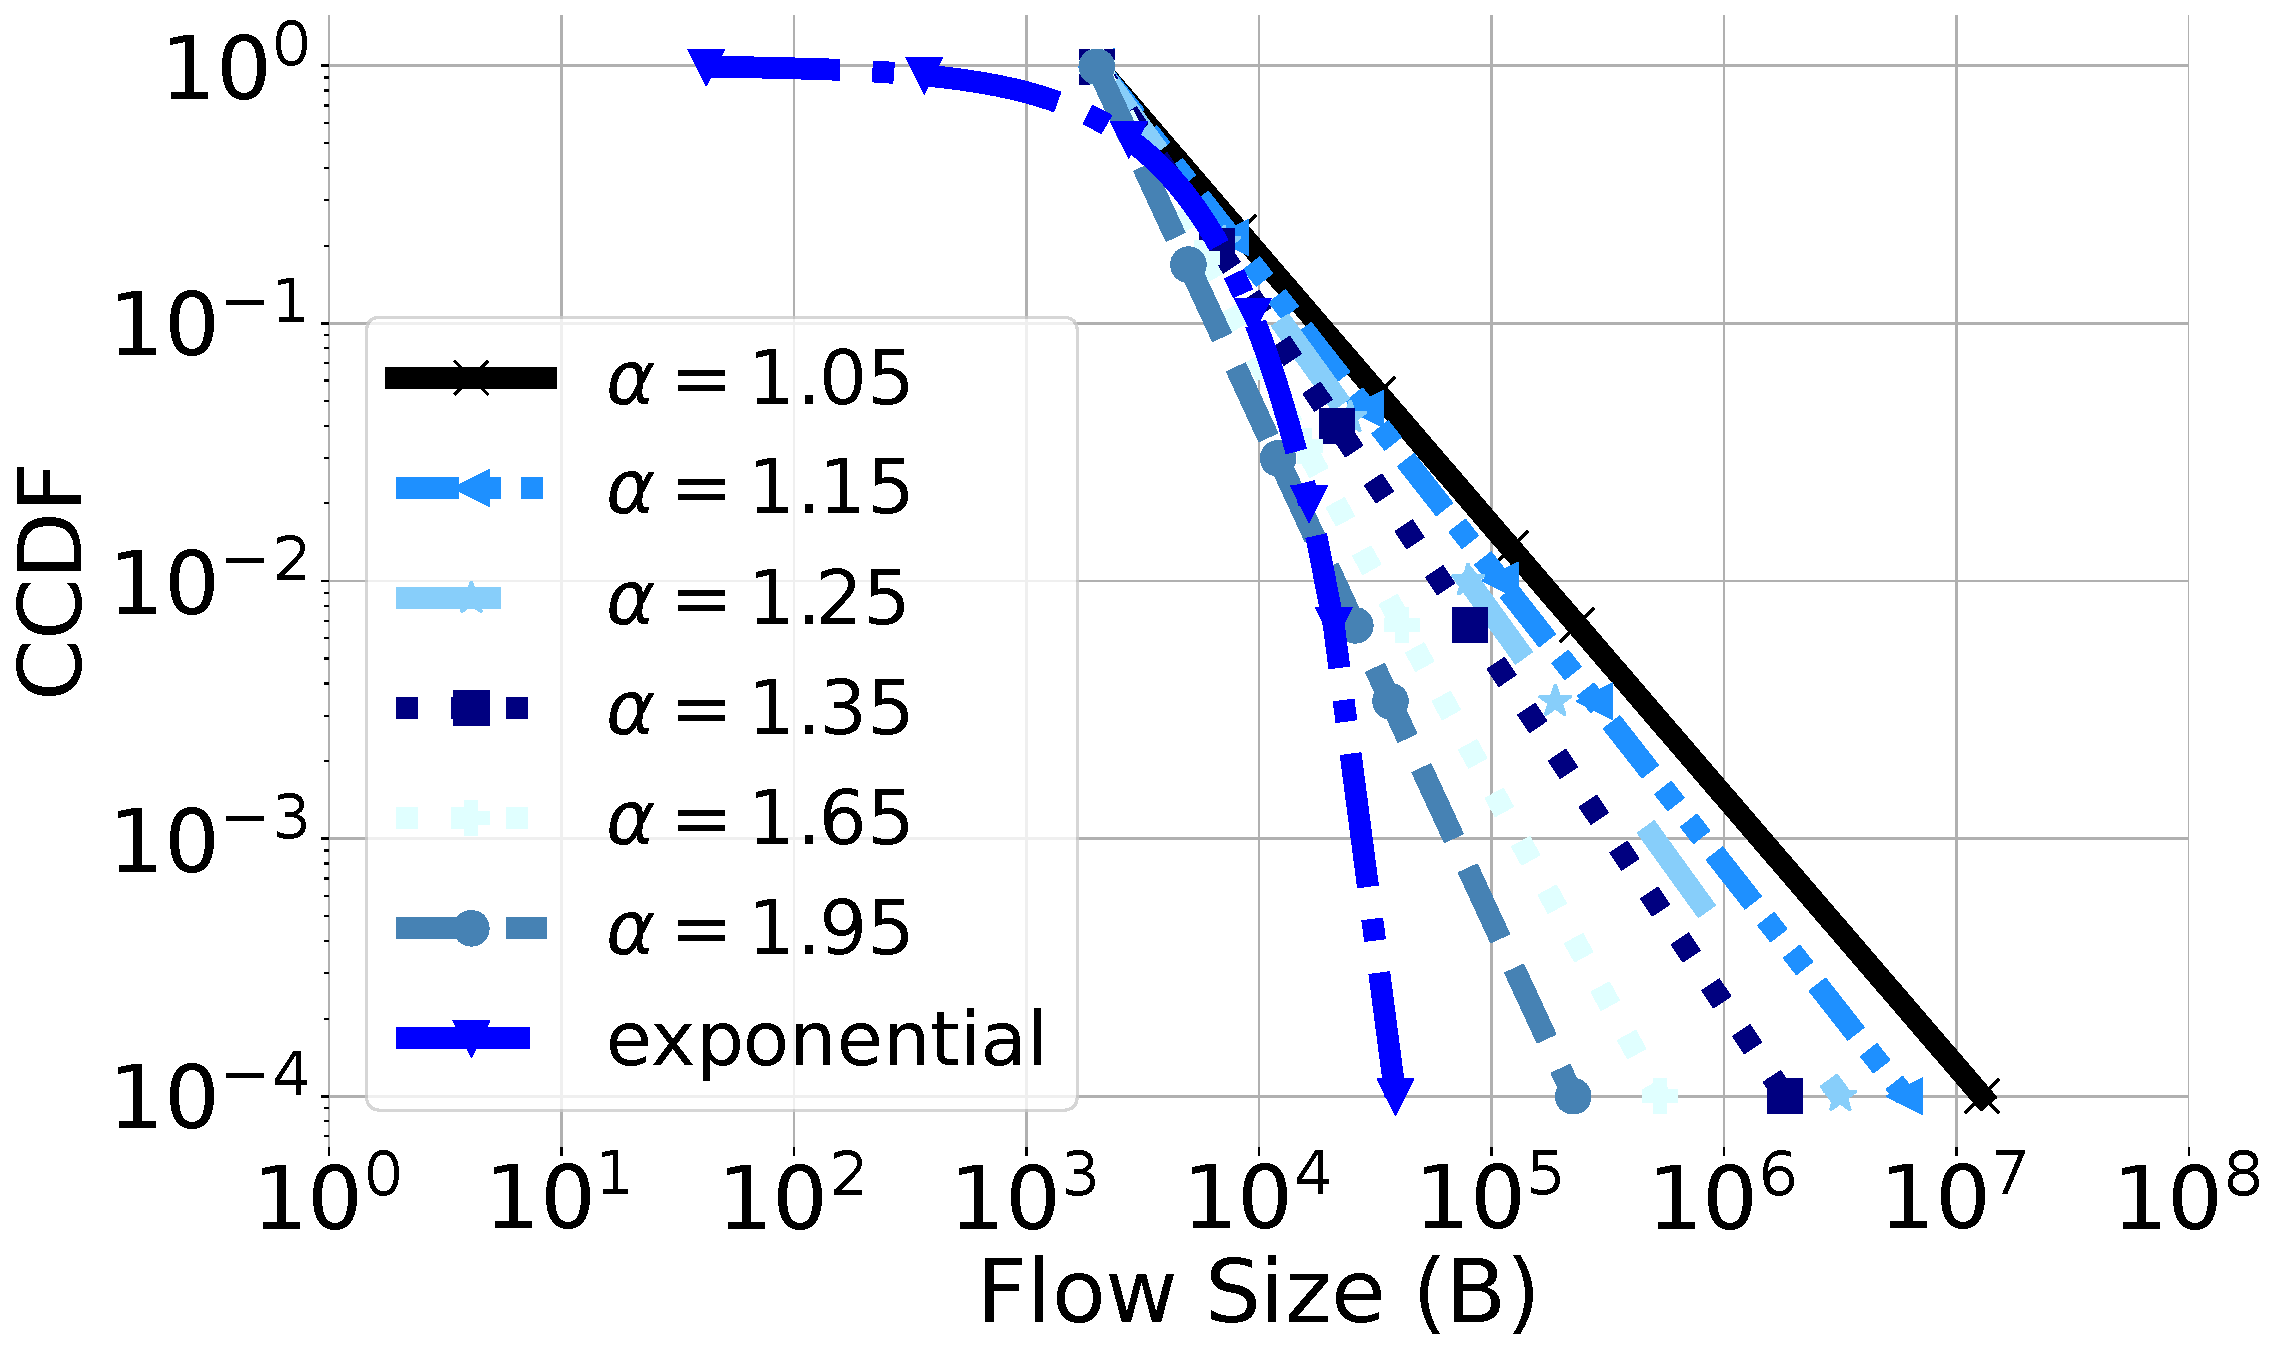
\includegraphics[width=1\linewidth]{figs/syntheticcdf_fsize_large.pdf}
    \caption{Synthetic workload}
	\label{fig:filecdf-dist}
\end{subfigure}
\begin{subfigure}[t]{0.49\linewidth}
    \centering
    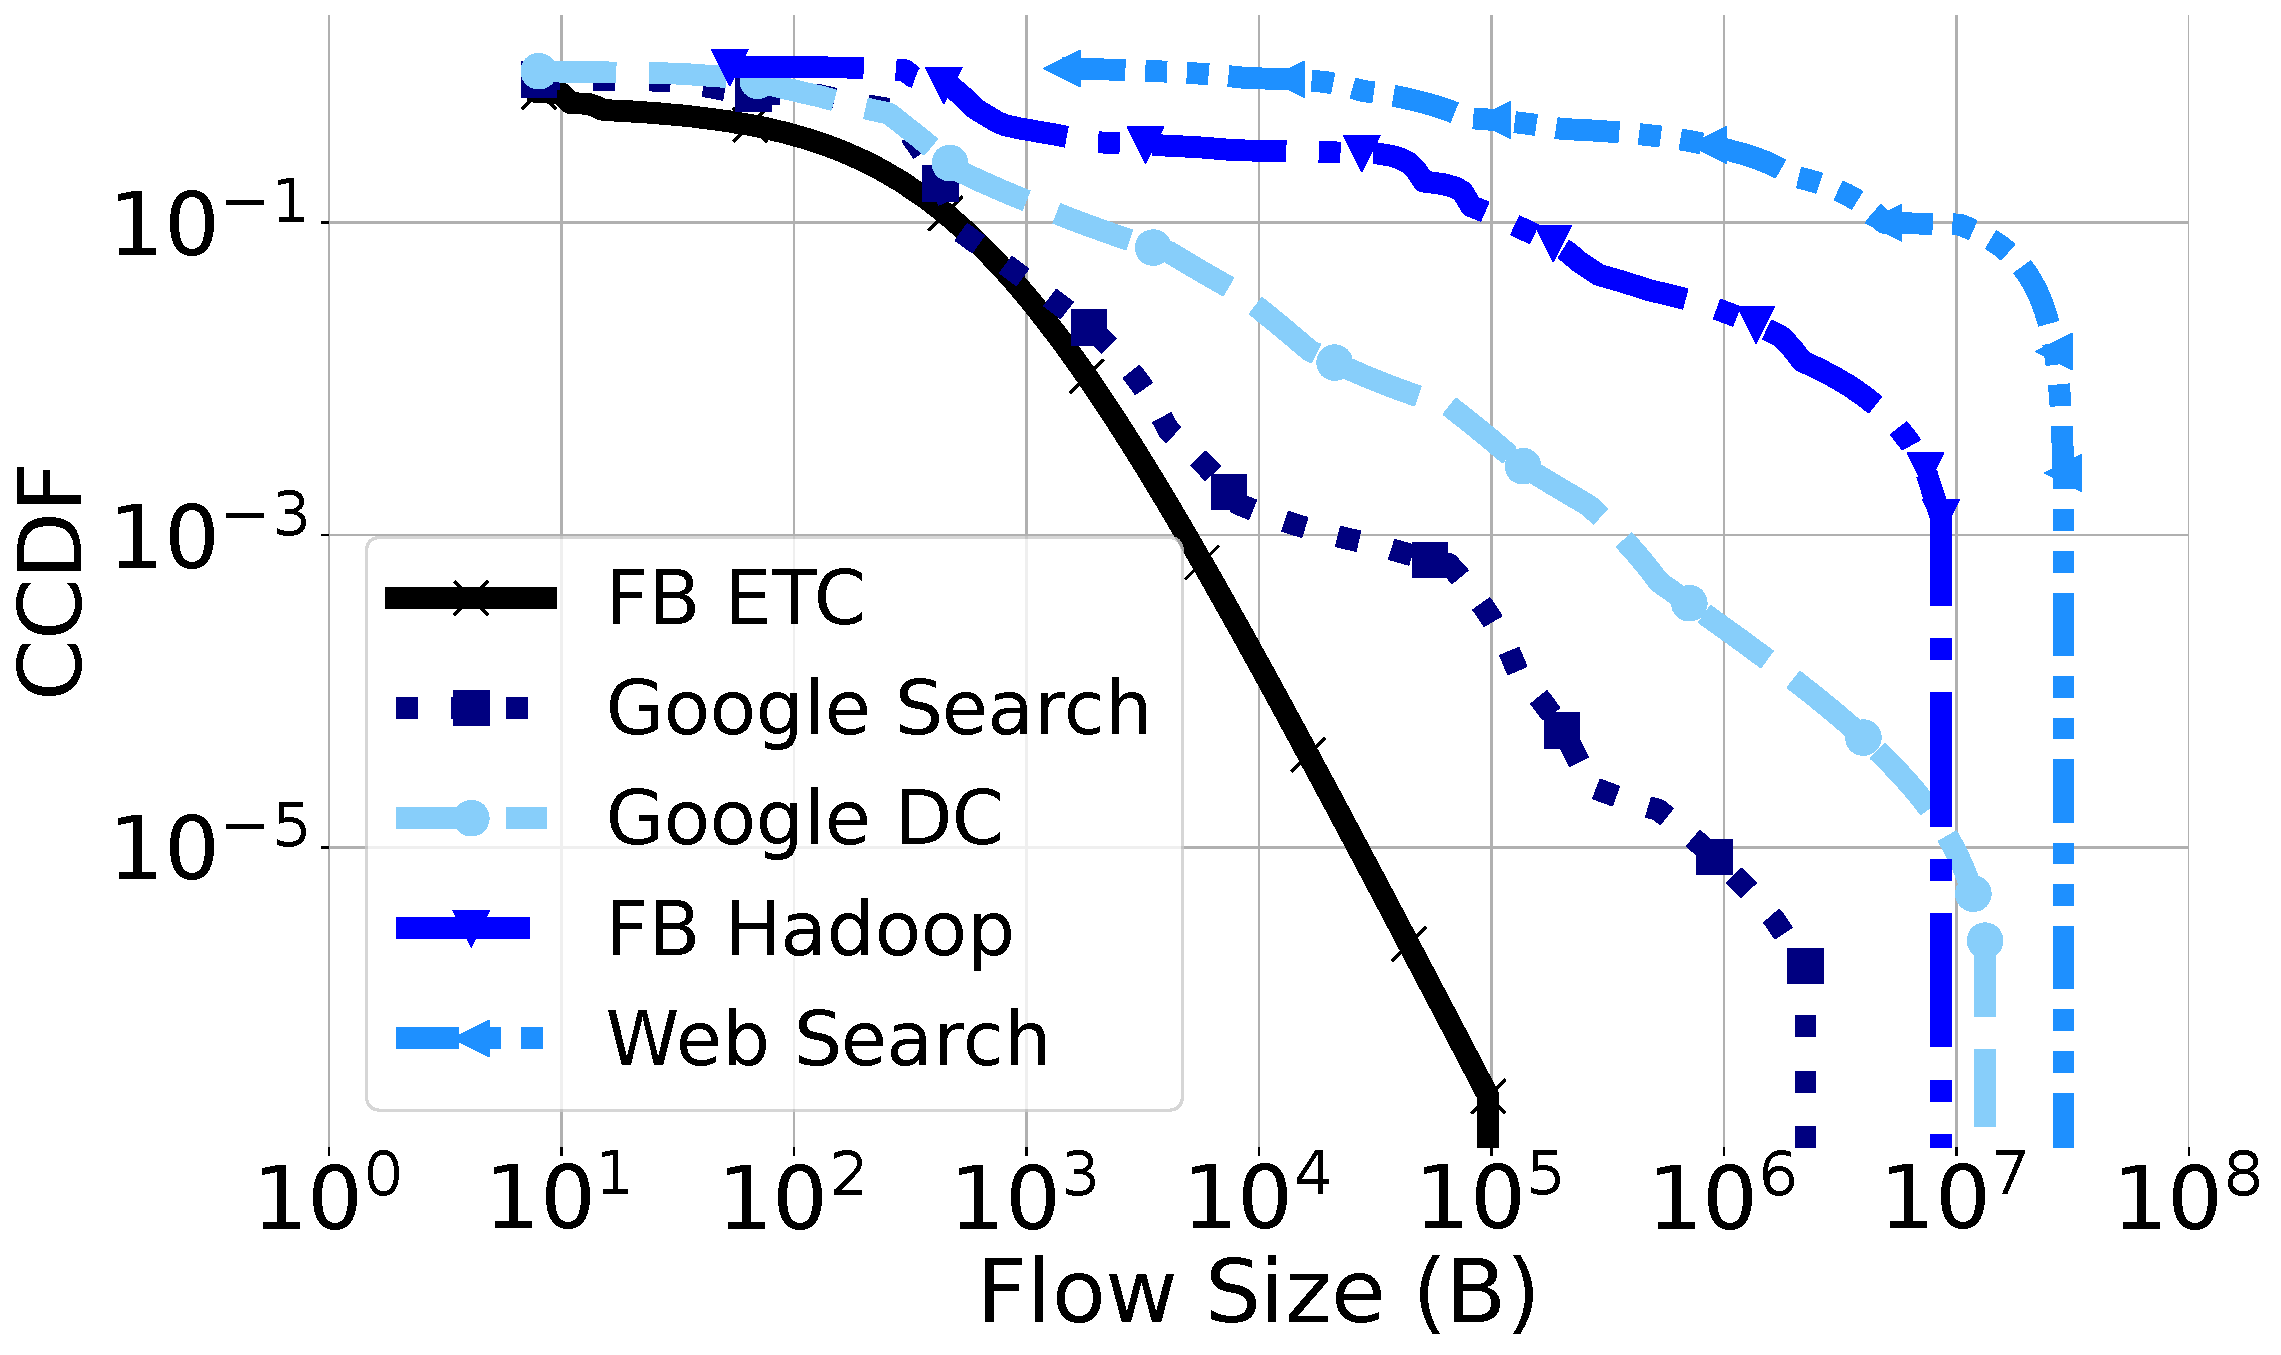
\includegraphics[width=1\linewidth]{figs/wccdf_fsize.pdf}
    \caption{Trace-driven workload}
	\label{fig:trace-ccdf}
\end{subfigure}
 % \vspace{-2mm}
    \caption{\small{Two sets of workloads used throughout the experiments. The figures show the complementary cumulative distribution functions (CCDFs) of flow sizes.}}
	\label{fig:distributions}
 % \vspace{-3mm}
\end{figure}


\begin{figure}[t]
\centering
\begin{subfigure}[t]{0.32\linewidth}
    \centering
    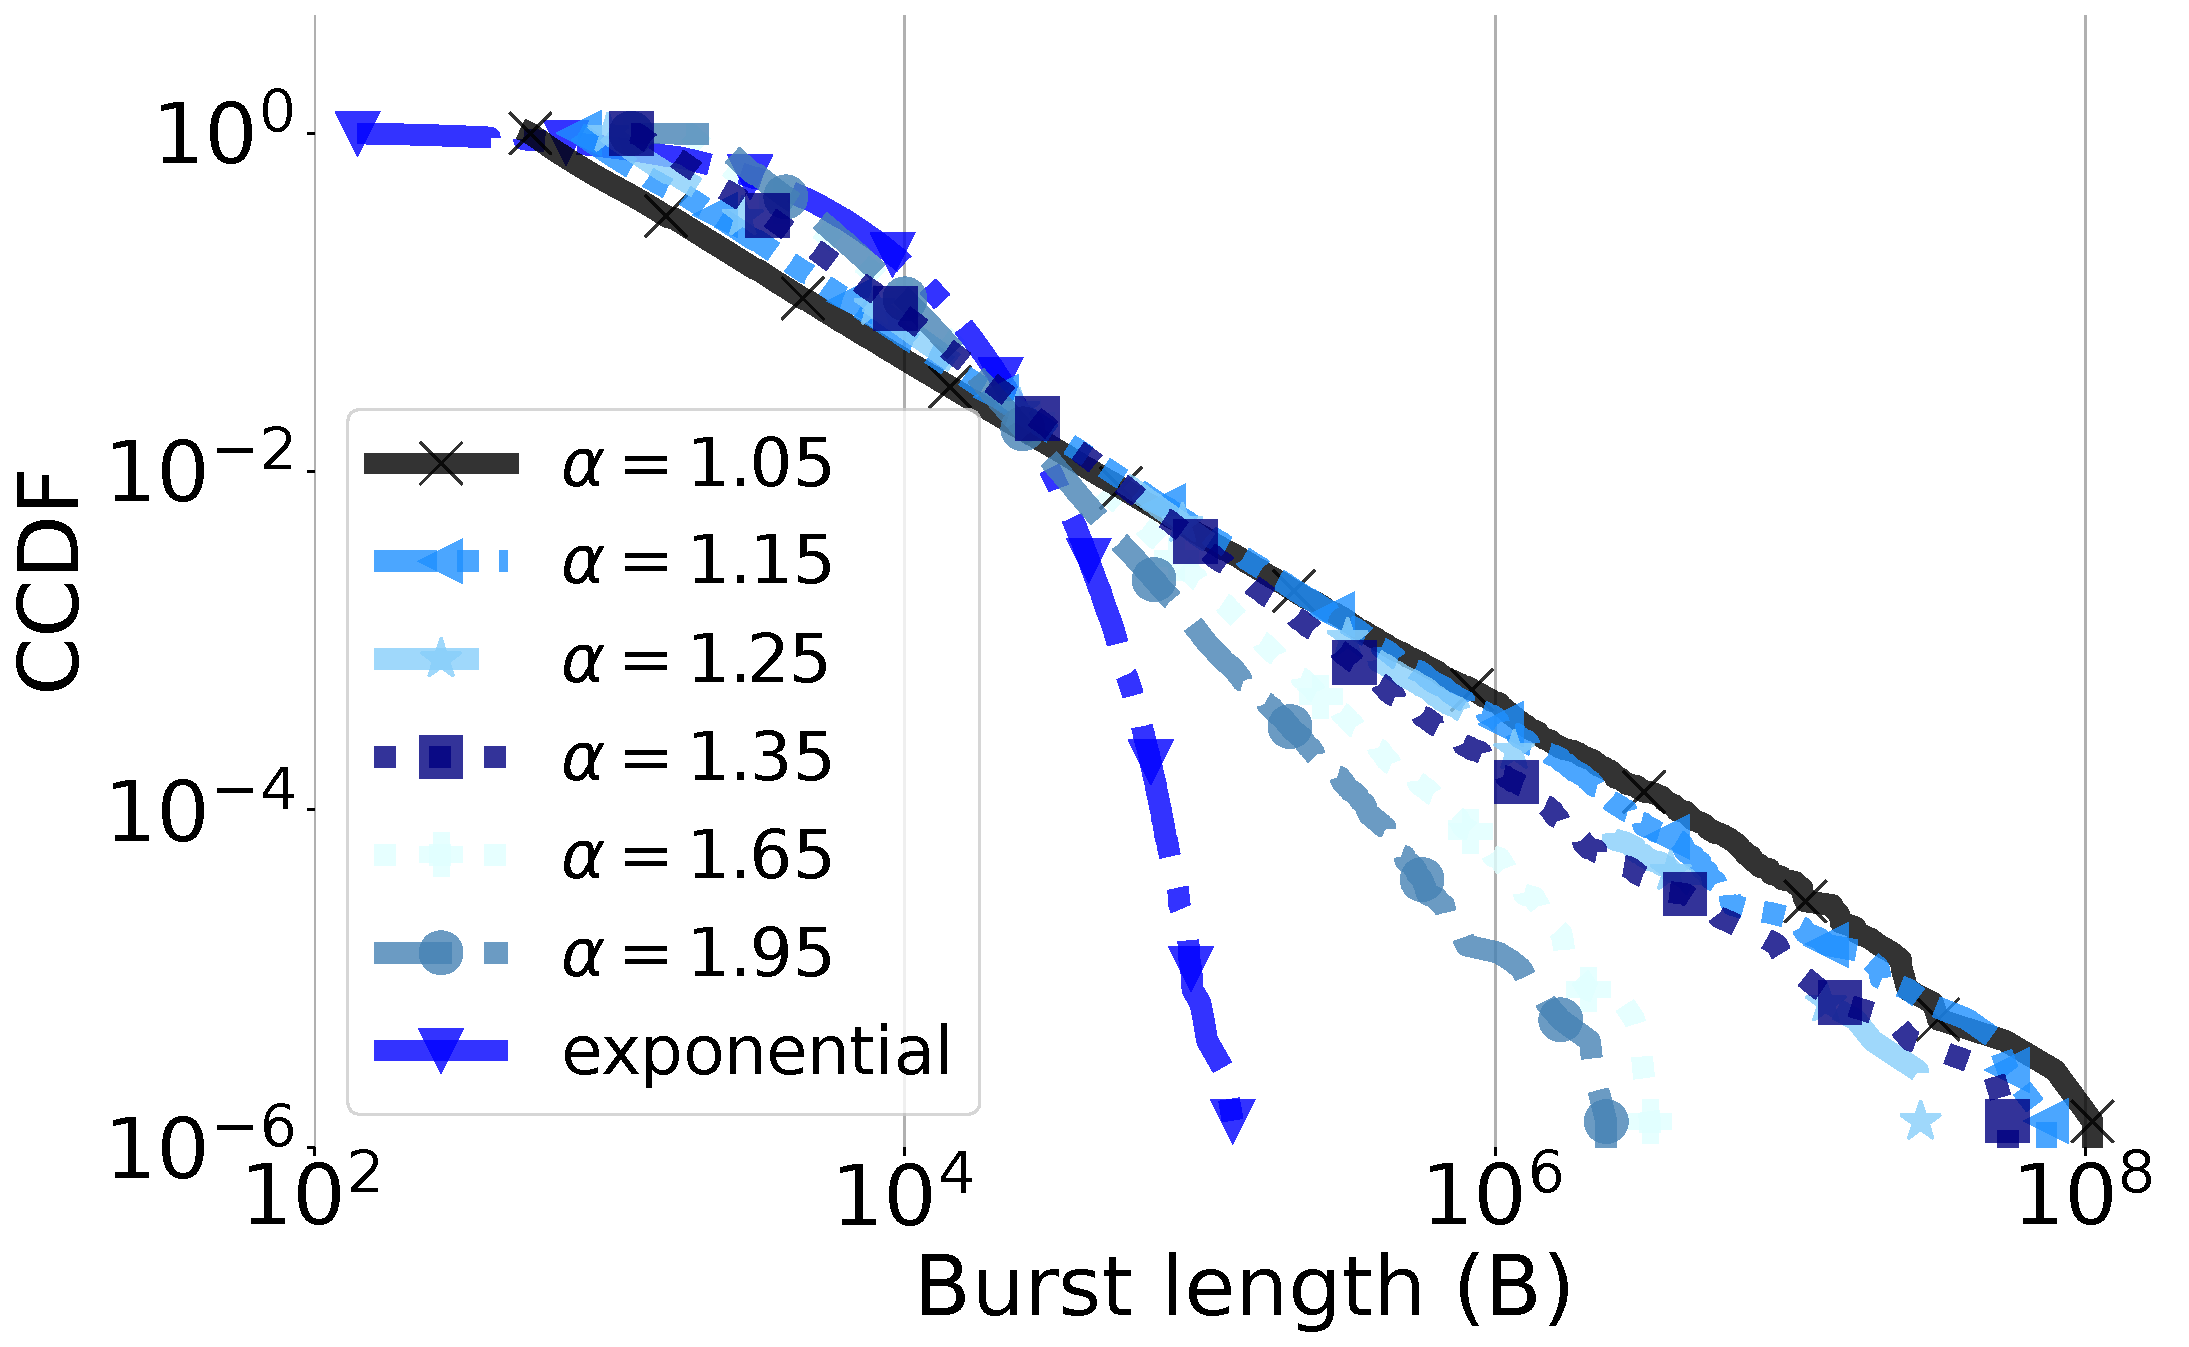
\includegraphics[width=1\linewidth]{figs/fileccdf_sim.pdf}
    \caption{Simulation microbursts}
	\label{fig:filecdf-sim}
\end{subfigure}
\begin{subfigure}[t]{0.32\linewidth}
    \centering
    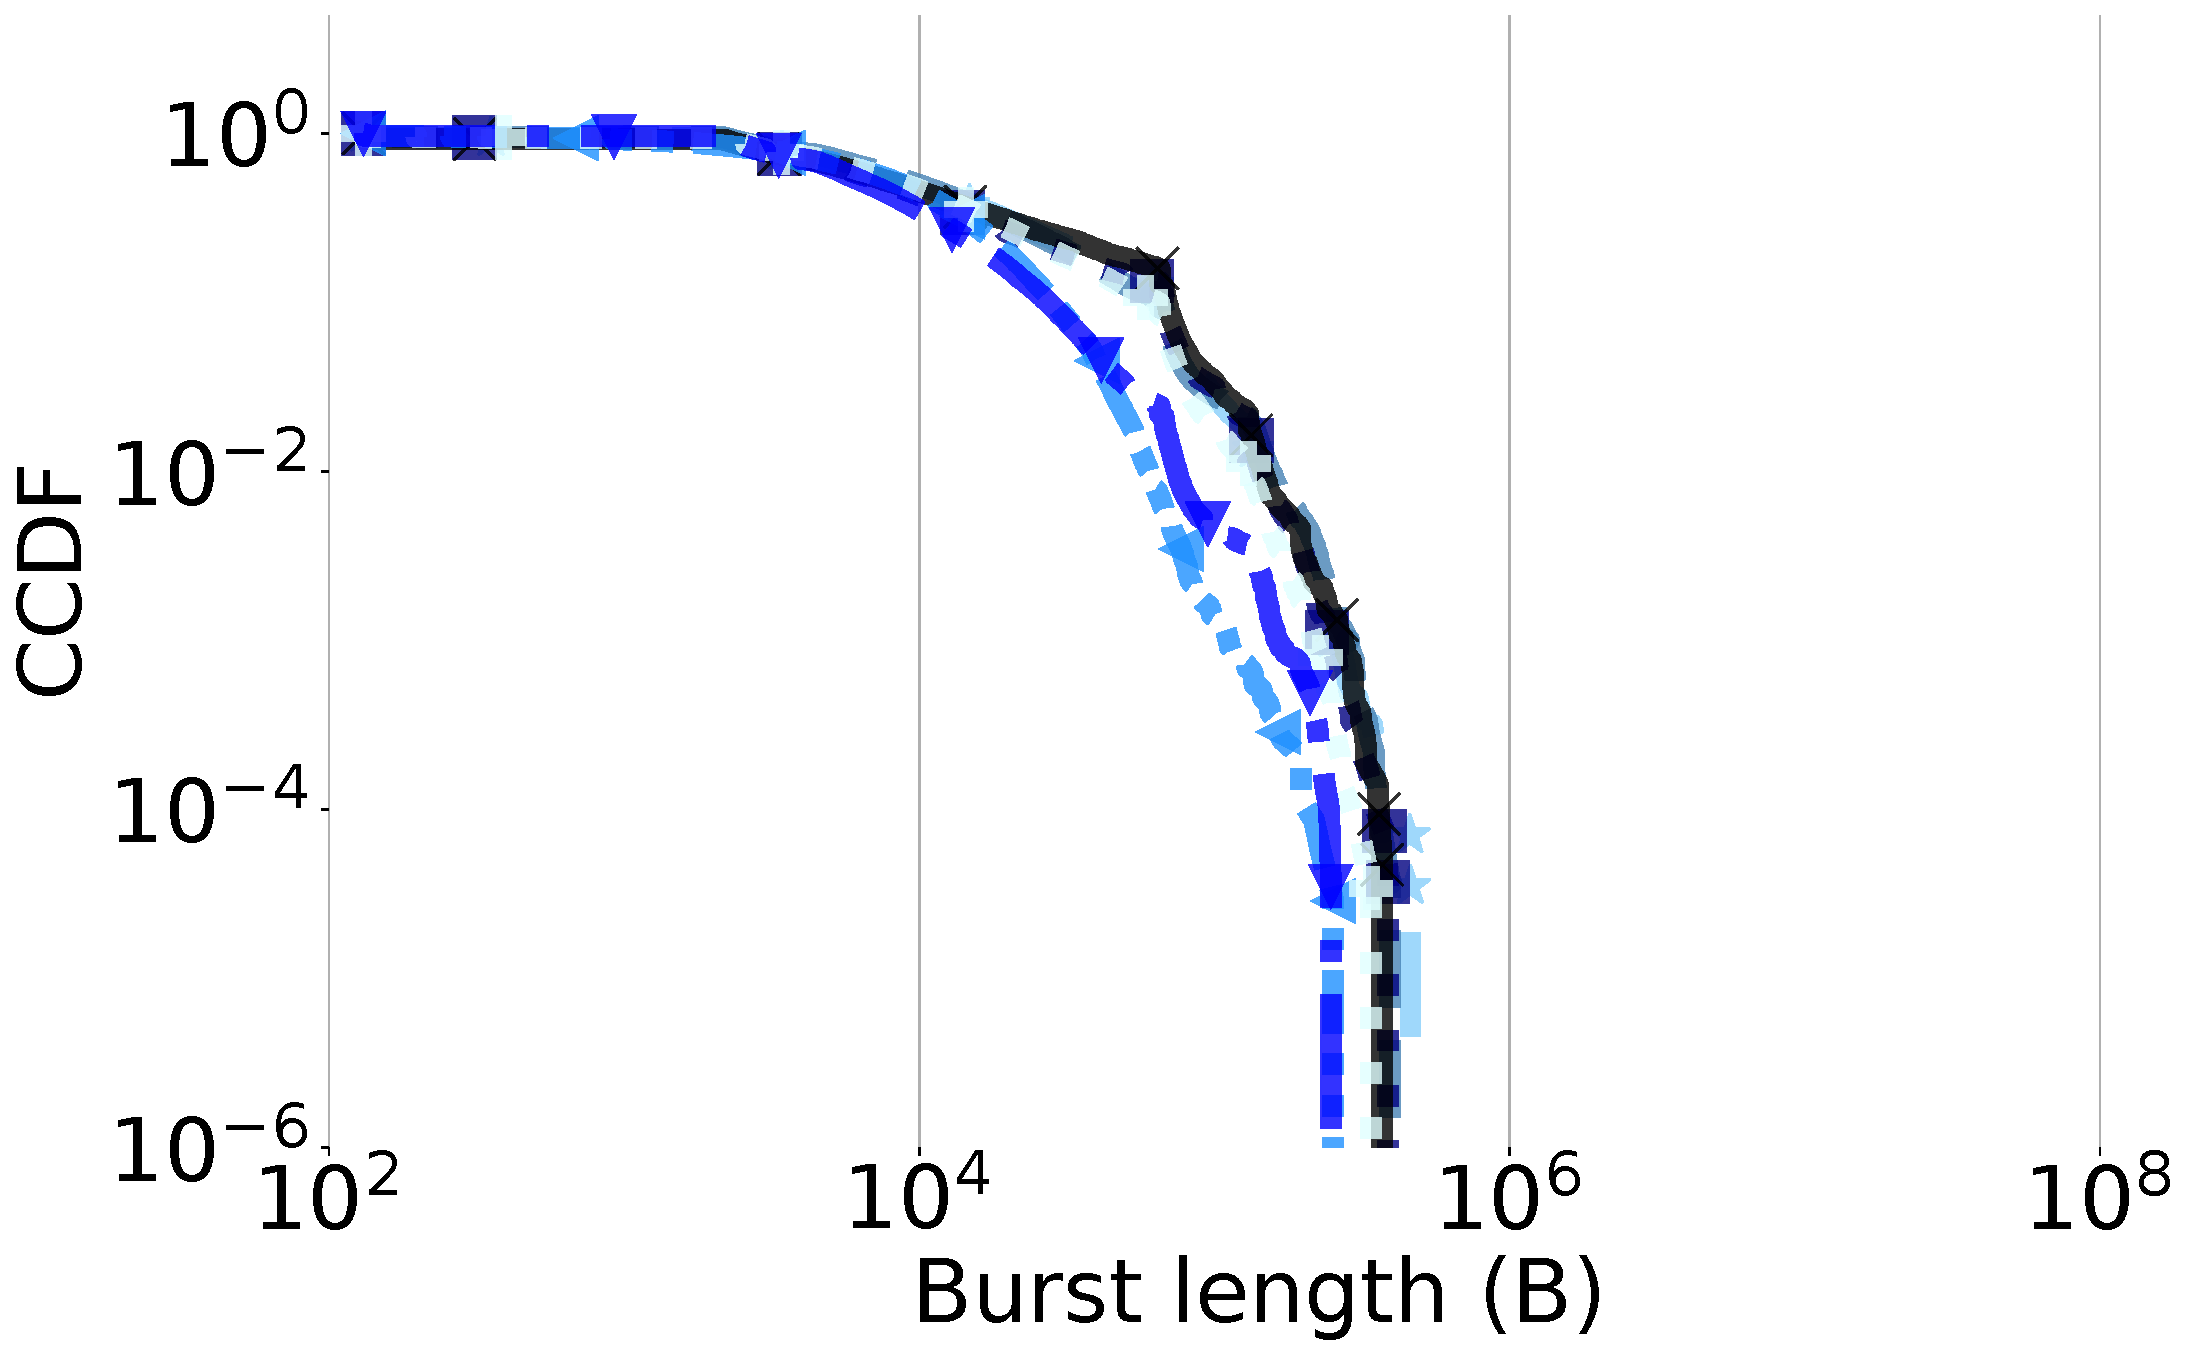
\includegraphics[width=1\linewidth]{figs/fileccdf_ebpf_testbed.pdf}
    \caption{In-host microbursts}
	\label{fig:fccdf-ebpf}
\end{subfigure}
\begin{subfigure}[t]{0.32\linewidth}
    \centering
    	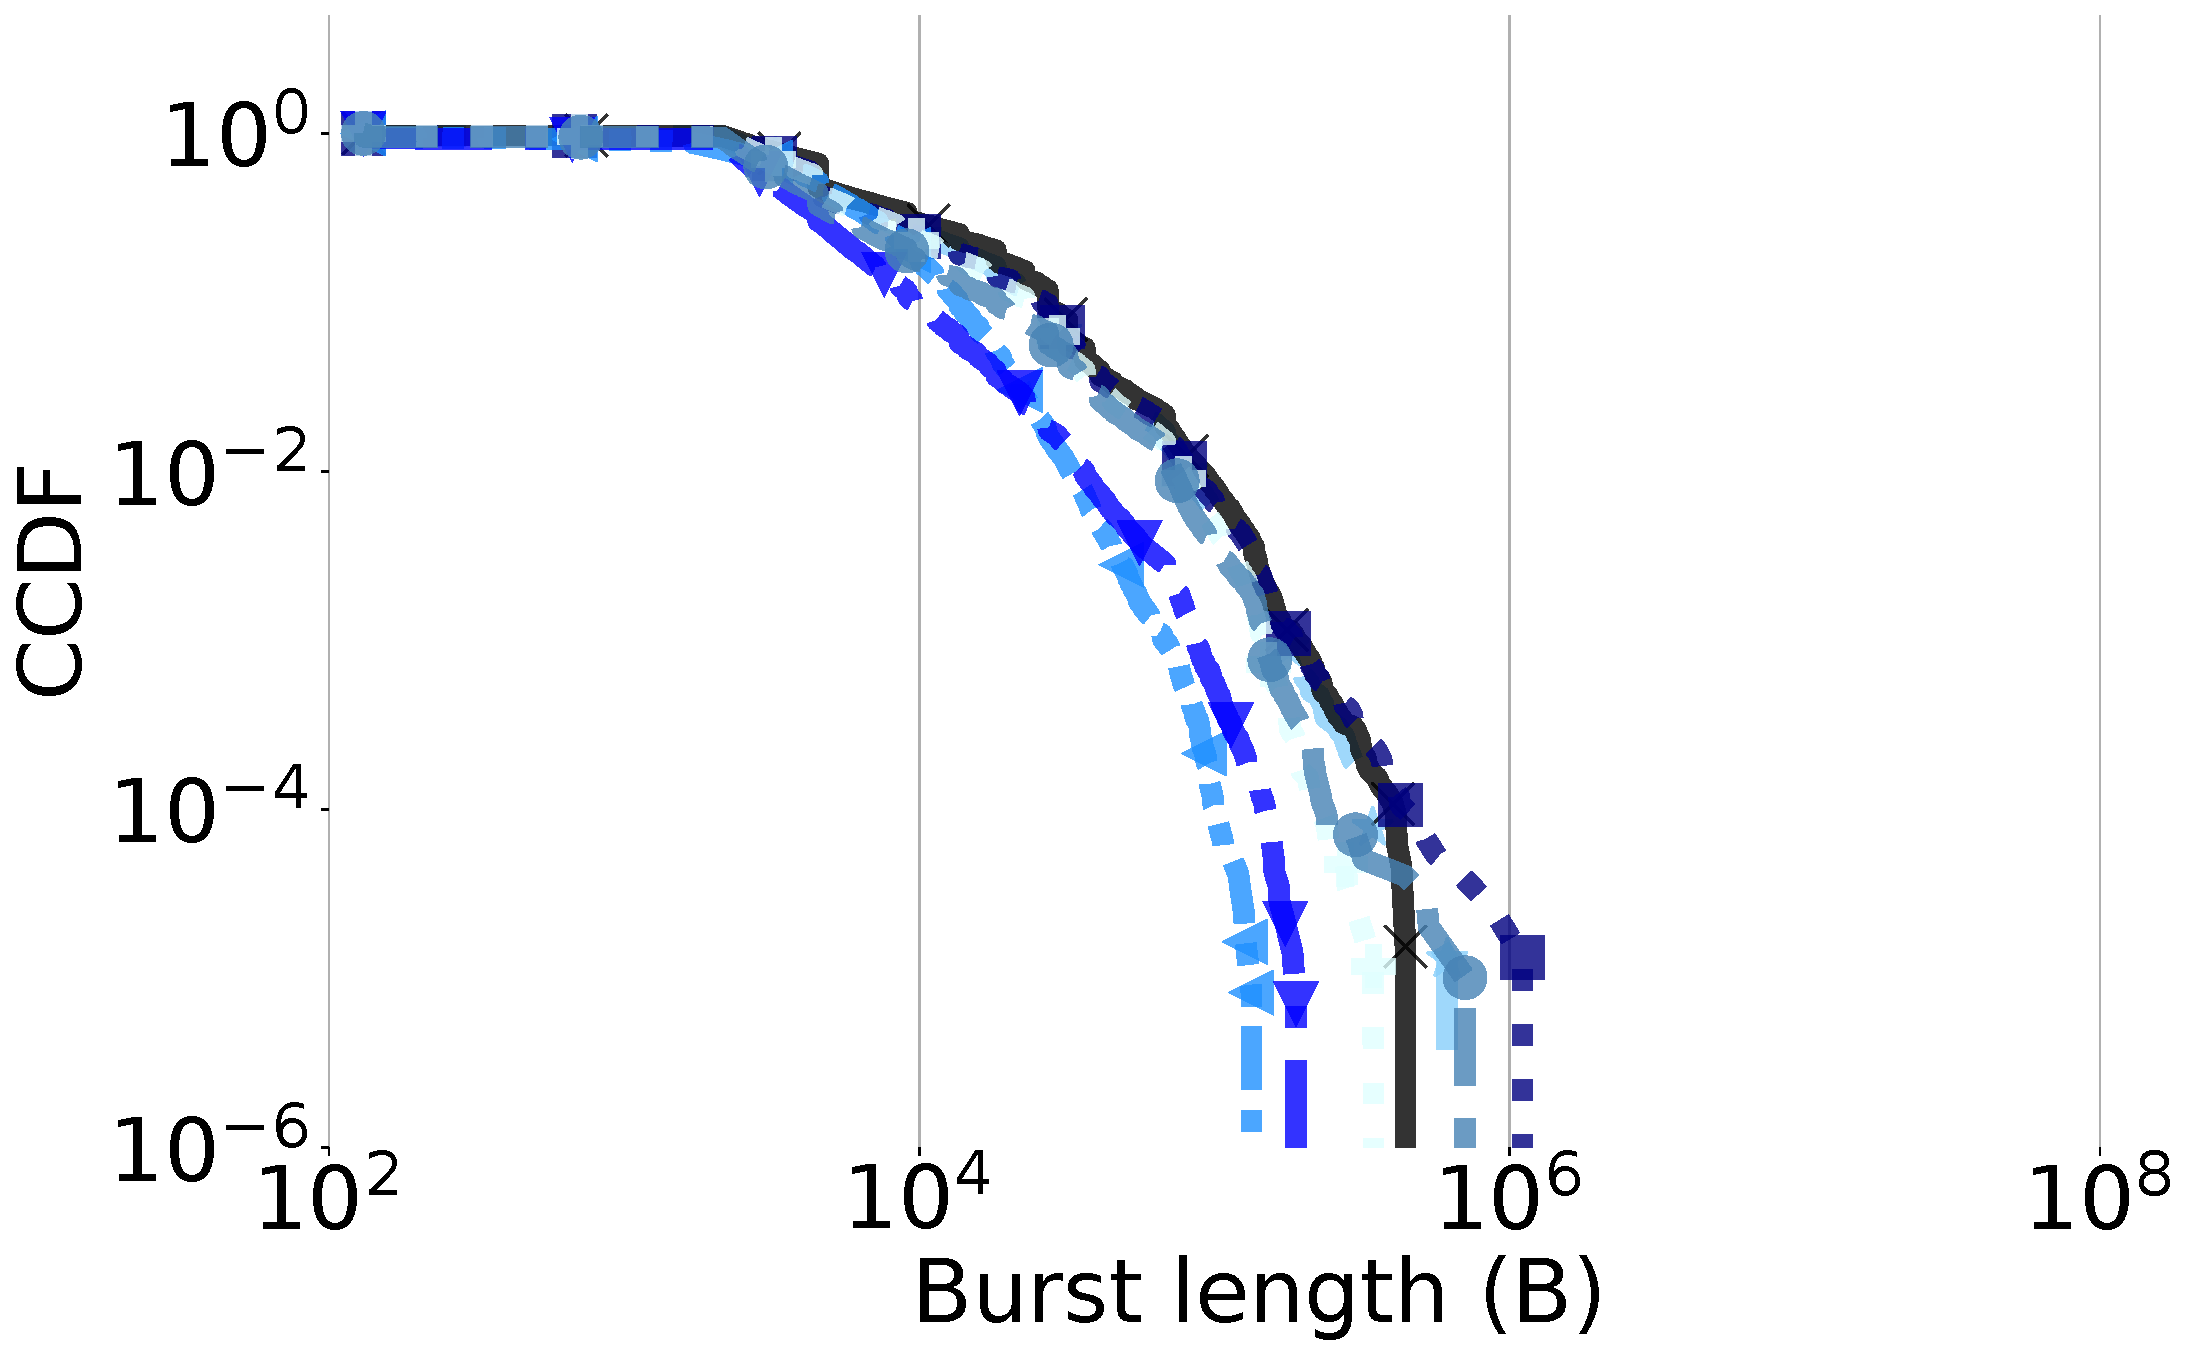
\includegraphics[width=1\linewidth]{figs/fileccdf_testbed.pdf}
    \caption{In-network microbursts}
	\label{fig:filecdf-testbed}
\end{subfigure}
\begin{subfigure}[t]{0.32\linewidth}
    \centering
    	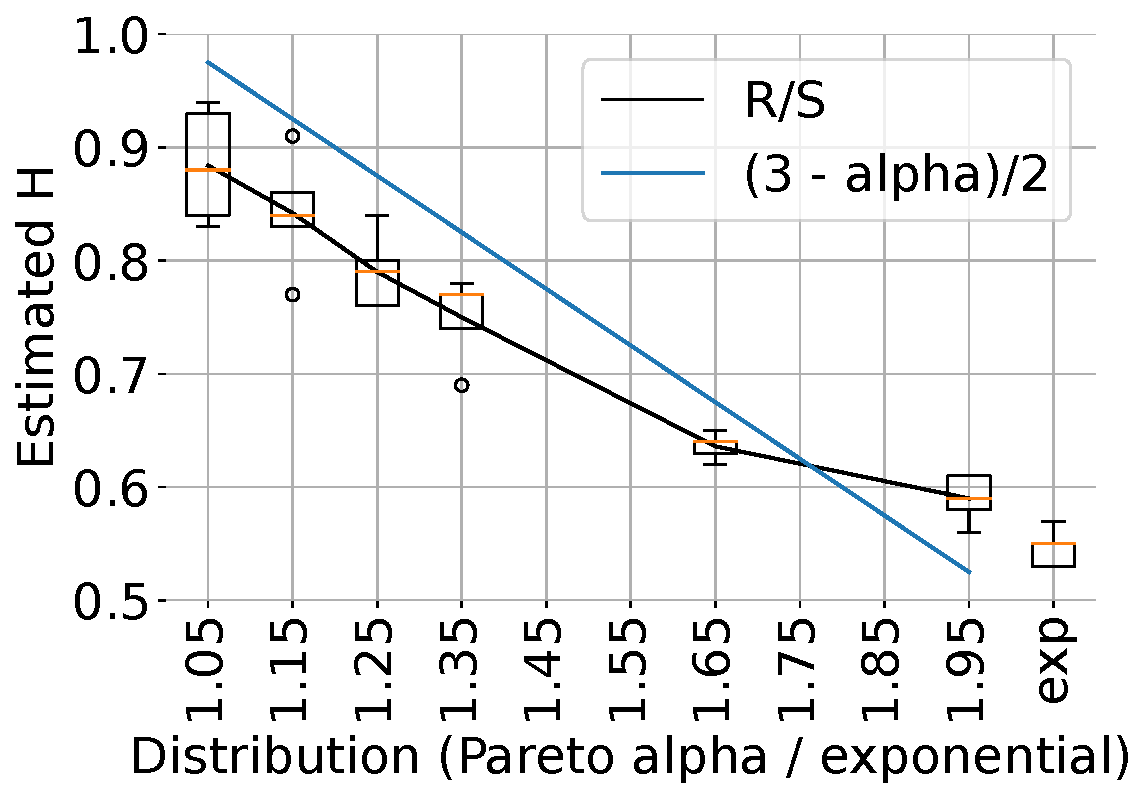
\includegraphics[width=1\linewidth]{figs/filehurst_sim.pdf}
    \caption{Simulation Hurst exp.}
	\label{fig:filehurst-sim}
\end{subfigure}
\begin{subfigure}[t]{0.32\linewidth}
    \centering
    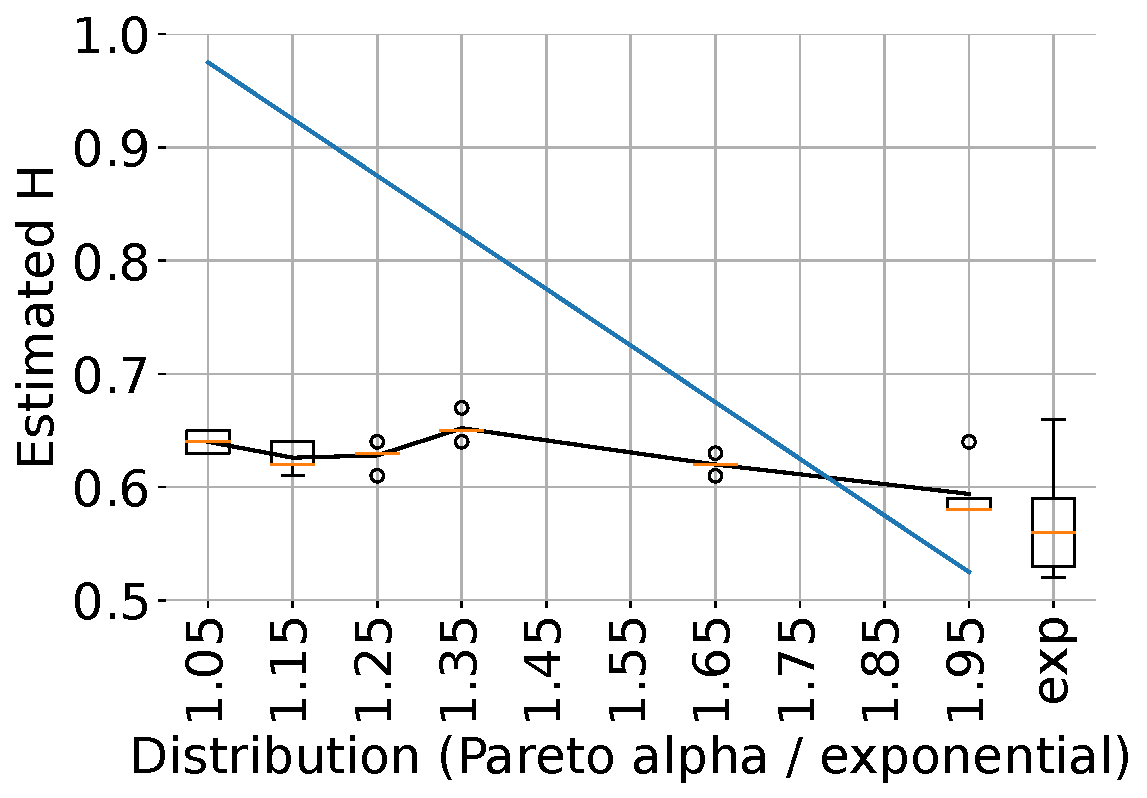
\includegraphics[width=1\linewidth]{figs/filehurst_ebpf_testbed.pdf}
    \caption{In-host Hurst exponents}
	\label{fig:fhurst-ebpf}
\end{subfigure}
\centering
\begin{subfigure}[t]{0.32\linewidth}
    \centering
    	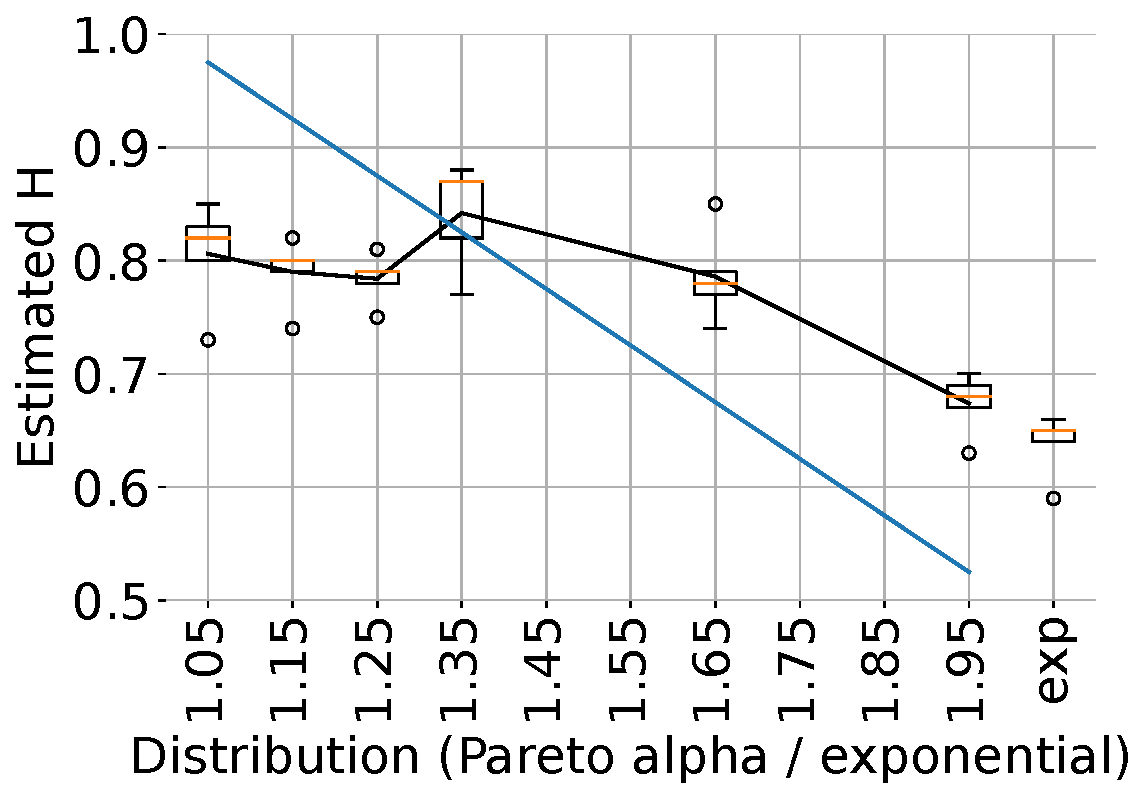
\includegraphics[width=1\linewidth]{figs/filehurst_testbed.pdf}
    \caption{In-network Hurst exp.}
	\label{fig:filehurst-testbed}
\end{subfigure}
 % \vspace{-2mm}
    \caption{\small{Microburst sizes and Hurst exponents of different synthetic workloads for simulated and testbed experiments are significantly different. 
    % The interference of host networking elements is visible in the difference between the three scenarios.
    }}
	\label{fig:filesize}
  % \vspace{-2mm}
\end{figure}

\subsection{Revisiting structural causality}
%Where does traffic burstiness come from? Is burstiness an artifact of application and workload internals, or is the host networking stack responsible for this temporal rise in traffic intensity at short time scales?
%To investigate, we run a network simulation, where 32 long-running TCP connections use Pareto and exponential flow size distributions depicted in Figure \ref{fig:filecdf-dist}. Flows are initiated exponentially and we set the distribution means in each case to make sure the offered load stays the same. We conduct all the simulations for five times in the OMNET \cite{omnet} simulator with a setup that imitates our physical testbed setting. According to \cite{filesize}, different $\alpha$ values for Pareto distributed flow sizes lead to different burstiness. Figure \ref{fig:filecdf-sim} testifies to the above claim. 
%While all synthetic flow size distributions have a mean of 4200KB, as Pareto $\alpha$ increases from 1.05 to 1.95, the heavy tail of the distribution is cut shorter and the size of bursts decreases accordingly. We observe that a light-tail distribution like exponential results in the lowest burstiness among all cases. The results in the CDF figure can also be interpreted by comparing the Hurst exponent estimates presented via the box-whisker plots in Figure \ref{fig:filehurst-sim}. 
%\erfan{Concretely, each box depicts the first and third quartiles of the estimated Hurst exponents for repeated simulation runs. The whiskers represent the upper and lower extremes, the circles are outlier points and the orange dashes present the mean values for Hurst estimates over multiple runs.}
%The trend in the rescaled-range estimates of Hurst exponents can be regressed to the (3$\alpha / 2$) line as we increase the $\alpha$ setting from 1.05 to 1.95.

%Next, we repeat the above scenario in a testbed, collecting the arrival timestamps both in the sending host and in the network. Figures \ref{fig:filecdf-testbed} and \ref{fig:filehurst-testbed} present the burst length distribution and Hurst estimates captured by Valinor-N in the network. Compared to the simulations, which lack the host network stack elements, Pareto $\alpha$ values that are lower than 1.95 result in almost the same amount of burstiness in the testbed. Only Pareto (1.95) and exponential cases are distinguishable since the p99 flow sizes in these two cases are 21KB and 18KB, respectively. Therefore, compared to the p99 flow size of 122KB for Pareto (1.05), they are less expected to produce trains of packets that form bursts. The trend in Hurst estimates also demonstrates that self-similarity does not follow the regressed (3$\alpha / 2$) line anymore.
%Finally, we report the in-host burstiness measurements of Valinor-H eBPF framework. The straight line between the boxes in Figure \ref{fig:fhurst-ebpf} suggests that the self-similarity of Pareto flows is further faded away as we remove the lower level components of the host networking stack from the picture (Valinor-H is placed before NIC processing in the stack). Compared to the in-network picture of burstiness, we observe that all the cases converge further to smaller H estimates (< 0.7). The burst length distributions in Figure \ref{fig:fccdf-ebpf} also conform to these findings.

Where does traffic burstiness come from?  
Prior work \cite{filesize, park1997effect, feldmann1999dynamics} shows that the heavy-tailed property of the flow size distribution directly determines link-level traffic self-similarity, a phenomenon that is sometimes referred to as \emph{structural causality}.  Heavy-tailed flow size distributions are shown to be the sufficient condition for generating scale-invariant burstiness and the network stack is shown to play a negligible role in self-similarity \cite{filesize, feldmann1999dynamics}. 
%
For instance, for traffic generated by TCP Reno for a heavy-tailed Pareto file size distribution with the shape parameter $\alpha$, there exists an almost linear relation between $H$ and $\alpha$: the estimated $H$ is close to $(3-\alpha)/2$.\footnote{The $H=(3-\alpha)/2$ relation shows the values of $H$ predicted by the a theoretical ON/OFF model in the idealized case corresponding to a fractional Gaussian noise process with independent traffic sources with constant ON/OFF amplitude \cite{park1997effect}. This captures an ideal self-similar process.} 
%with a slightly lower slope, an offset below the idealized line for $\alpha$ close to 1 (more heavy-tailed), and above the line for $\alpha$ close to 2 (less heavy-tailed).
Heavier tailed distributions (i.e., $\alpha$ close to 1) are more strongly self-similar ($H$ closer to 1). The self-similarity of traffic with heavy-tailed flow sizes is in contrast to the lack of correlation structures for short-tailed flow size distributions such as an exponential distribution ($H$ close to 0.5).

We first replicate this result using OMNET \cite{omnet}, an extensively used simulator \cite{homa,conga,fatpaths}, and observe an almost linear relation between $\alpha$ and $H$---consistent with the findings of prior work \cite{filesize}, the estimated $H$ values closely track the $(3-\alpha)/2$ line. In a setup where the two simulated servers are connected via a network switch, we establish 32 long-running TCP connections and use Pareto and exponential flow size distributions (Figure \ref{fig:filecdf-dist} shows the flow size distributions). To achieve a target offered load of 6 Gbps, flows are initiated exponentially with a mean interarrival time of 87$\mu$s. We repeat each experiment five times. In the box and whisker plots, each box depicts the $1^{st}$ and $3^{rd}$ quartiles, the whiskers represent the upper and lower extremes, the circles are outlier points, and the orange dashes show the median Hurst estimates. Figure \ref{fig:filehurst-sim} shows that heavy-tailed flow size distributions generate self-similar traffic. Figure \ref{fig:filecdf-sim} shows that these distributions also result in larger microbursts with heavier tails.

Next, we repeat the above scenario in a testbed, using Valinor to analyze burstiness after the software stack and on the wire. Using Valinor-H for in-host analysis, we observe that the impact of the heavy-tailed distributions on self-similarity is barely visible at this stage with distributions with varying $\alpha$ parameters behaving similarly and close to a light-tail exponential distribution (Figure \ref{fig:fhurst-ebpf}), e.g., the software stack greatly diminishes the degree of self-similarity of heavy-tailed Pareto distribution with $\alpha=1.05$ from $H=0.88$ in the simulations (Figure \ref{fig:filehurst-sim}) to $H=0.64$ at the eBPF hook (Figure \ref{fig:fhurst-ebpf}). We observe a similar effect on the microburst size distributions that are much more similar across different workloads and have shorter tails (Figure \ref{fig:fccdf-ebpf}).

We next use Valinor-N for analyzing traffic as observed on the wire. The patterns again change in interesting and non-uniform ways. Similar to in-host measurements, the in-network measurements indicate that the influence of flow size on self-similarity is lower than the simulated experiments, e.g., $H=0.80$ and $H=0.78$ for $\alpha=1.05$ and $\alpha=1.65$, respectively, on the wire in the testbed experiments compared to $H=0.88$ and $H=0.63$ for the same workloads in the simulated experiments (Figure \ref{fig:filehurst-testbed}). The more amplified long-range burstiness in the network compared to in-host experiments is due to the intervention of driver and NIC functions (such as segmentation offloading scheduling) that reside below Valinor-H. We investigate the roles of these functions in \S\ref{sec:sources}. 
%
Figure \ref{fig:filecdf-testbed} shows that the flow size distribution has a relatively subdued impact on the ultimate size of microbursts on the wire once the traffic traverses the host networking stack.

\paragraph{Summary:} The shape of the traffic in the testbed experiments (in-network and in-host) is substantially different compared to the simulated experiments with identical setups. This suggests that host networking elements (e.g., qdiscs, process schedulers, and NIC schedulers, not modeled in common simulators) alter burstiness.

\begin{figure}[t]
\centering
\begin{subfigure}[t]{0.40\linewidth}
    \centering
    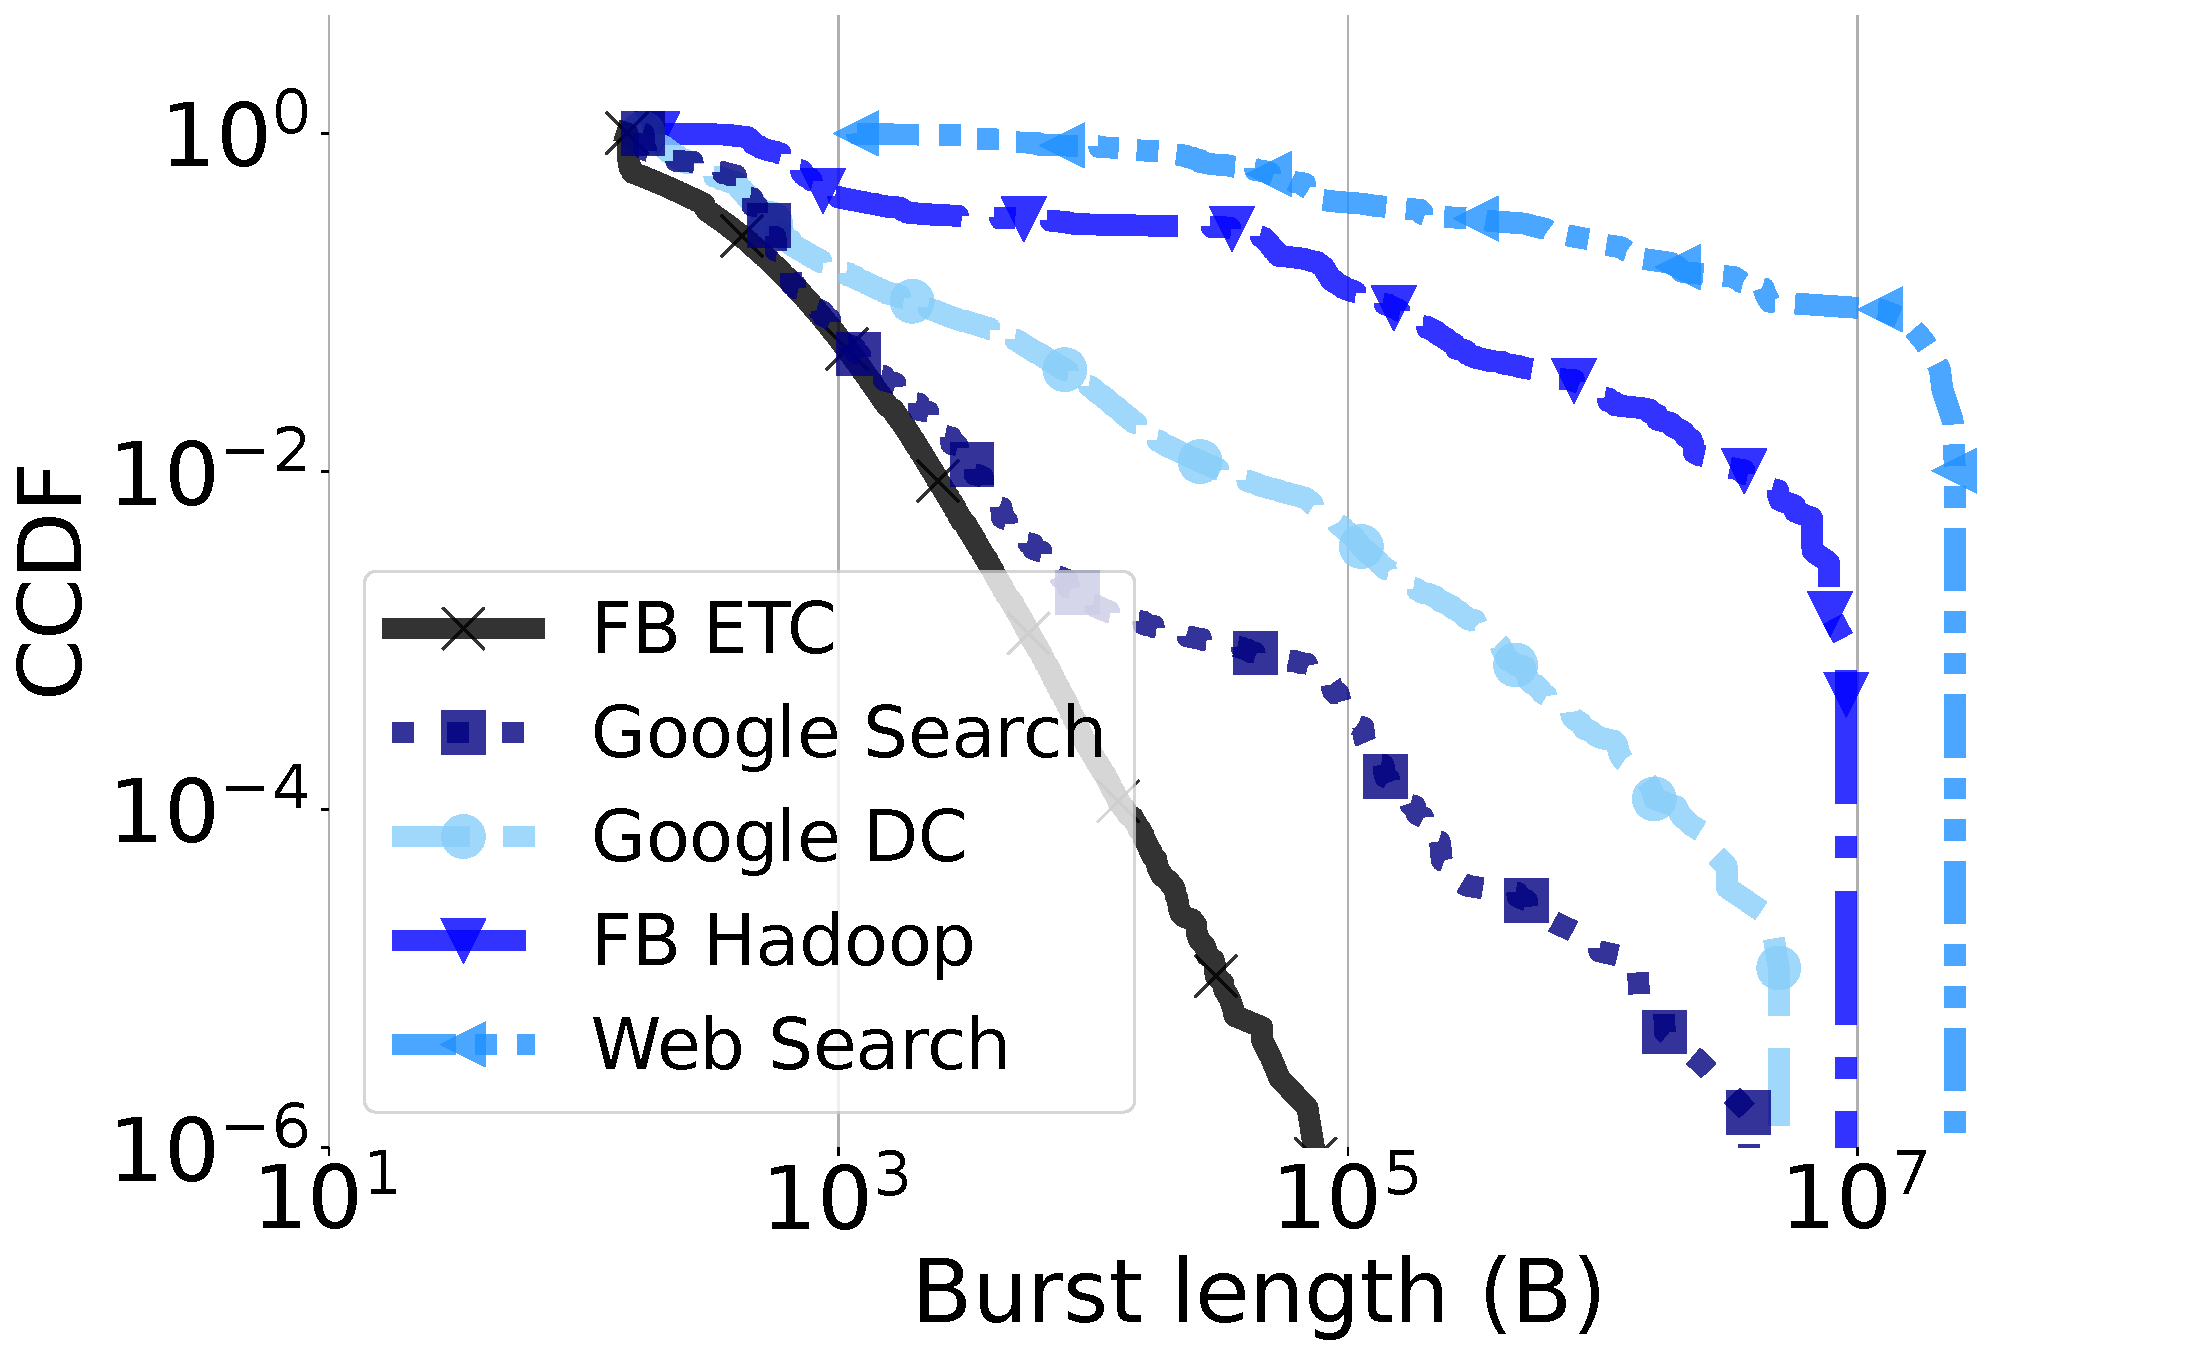
\includegraphics[width=1\linewidth]{figs/wccdf_sim.pdf}
    \caption{Simulation microburst sizes}
	\label{fig:wcdf-sim}
\end{subfigure}
\begin{subfigure}[t]{0.40\linewidth}
    \centering
    	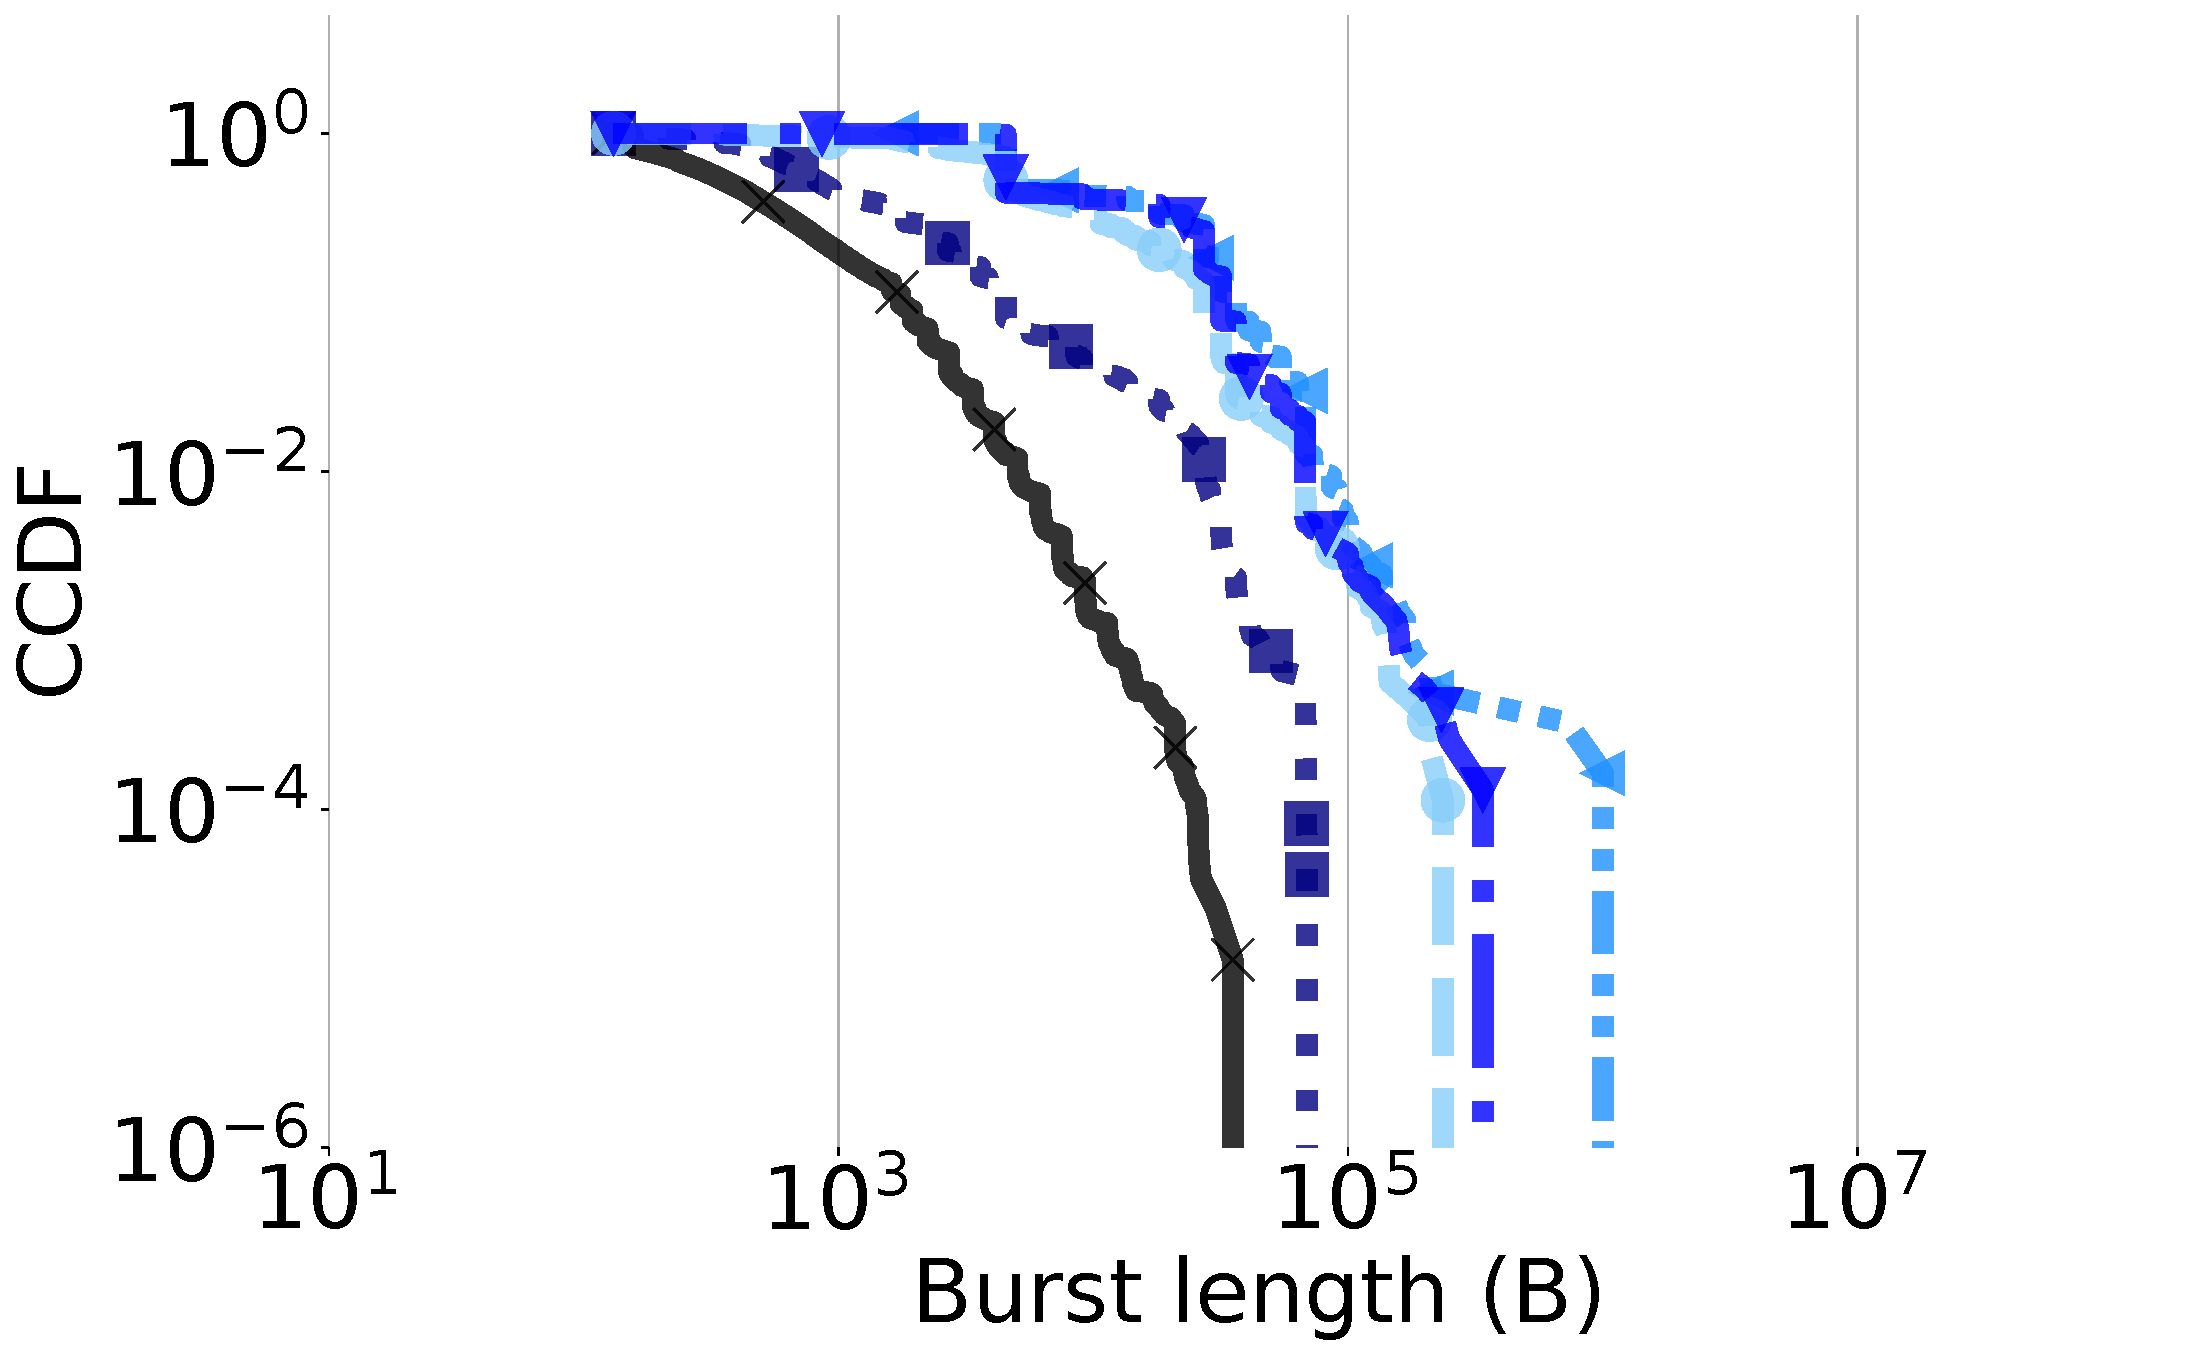
\includegraphics[width=1\linewidth]{figs/wccdf_testbed.pdf}
    \caption{In-network microburst sizes}
	\label{fig:wcdf-testbed}
\end{subfigure}
\begin{subfigure}[t]{0.40\linewidth}
    \centering
    	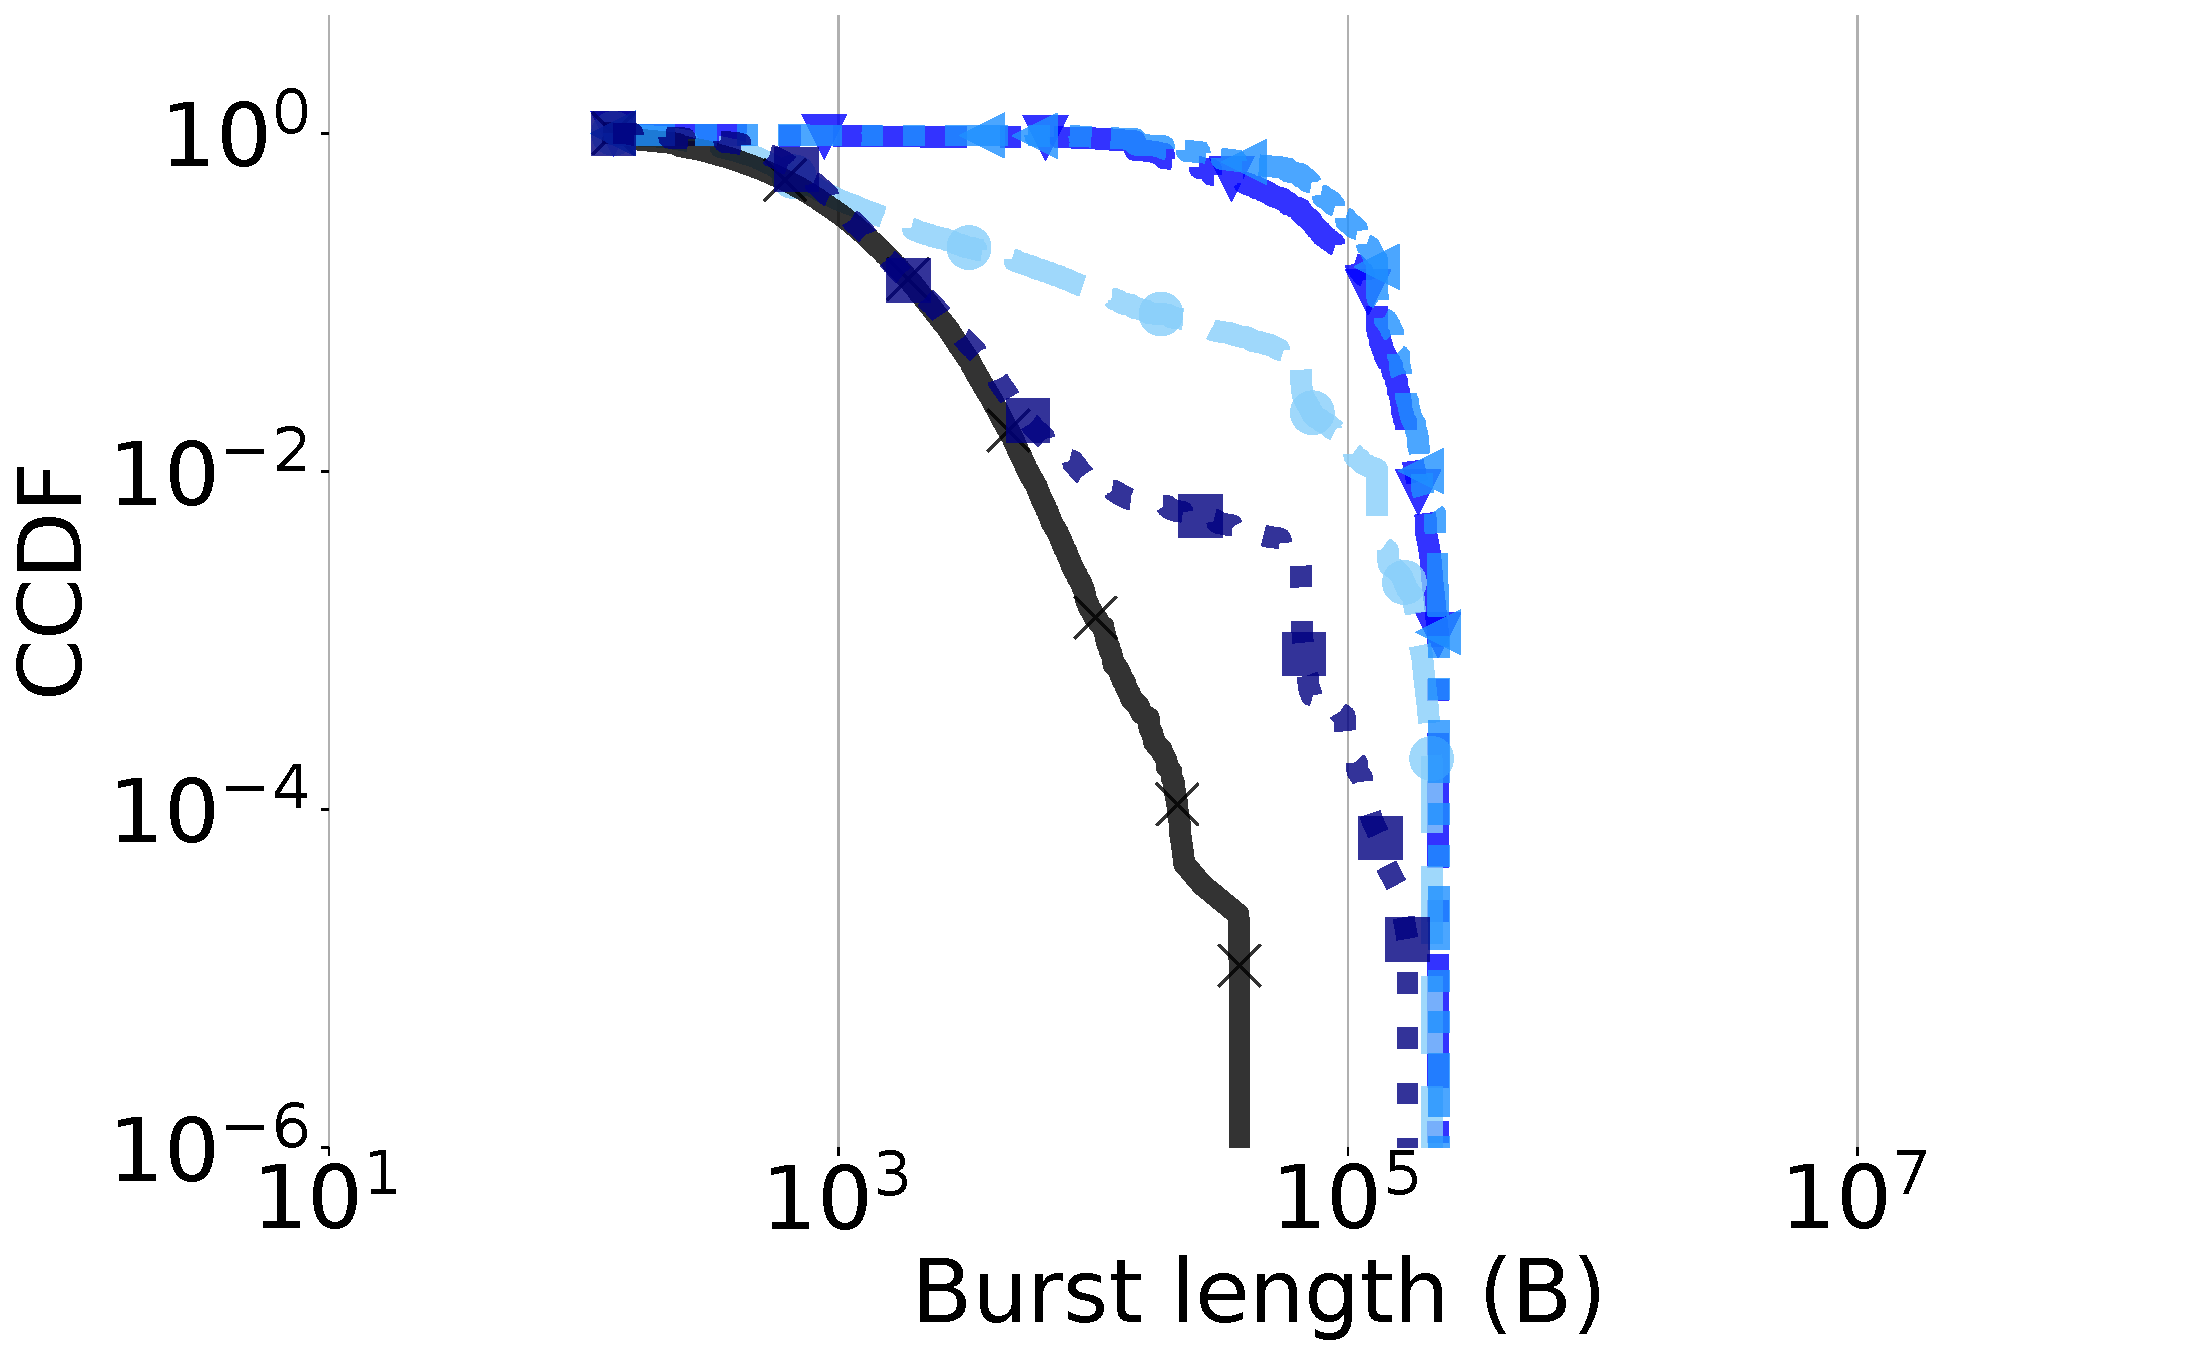
\includegraphics[width=1\linewidth]{figs/wccdf_ebpf_testbed.pdf}
    \caption{In-host microburst sizes}
	\label{fig:fwccdf-ebpf}
\end{subfigure}
\begin{subfigure}[t]{0.36\linewidth}
    \centering
    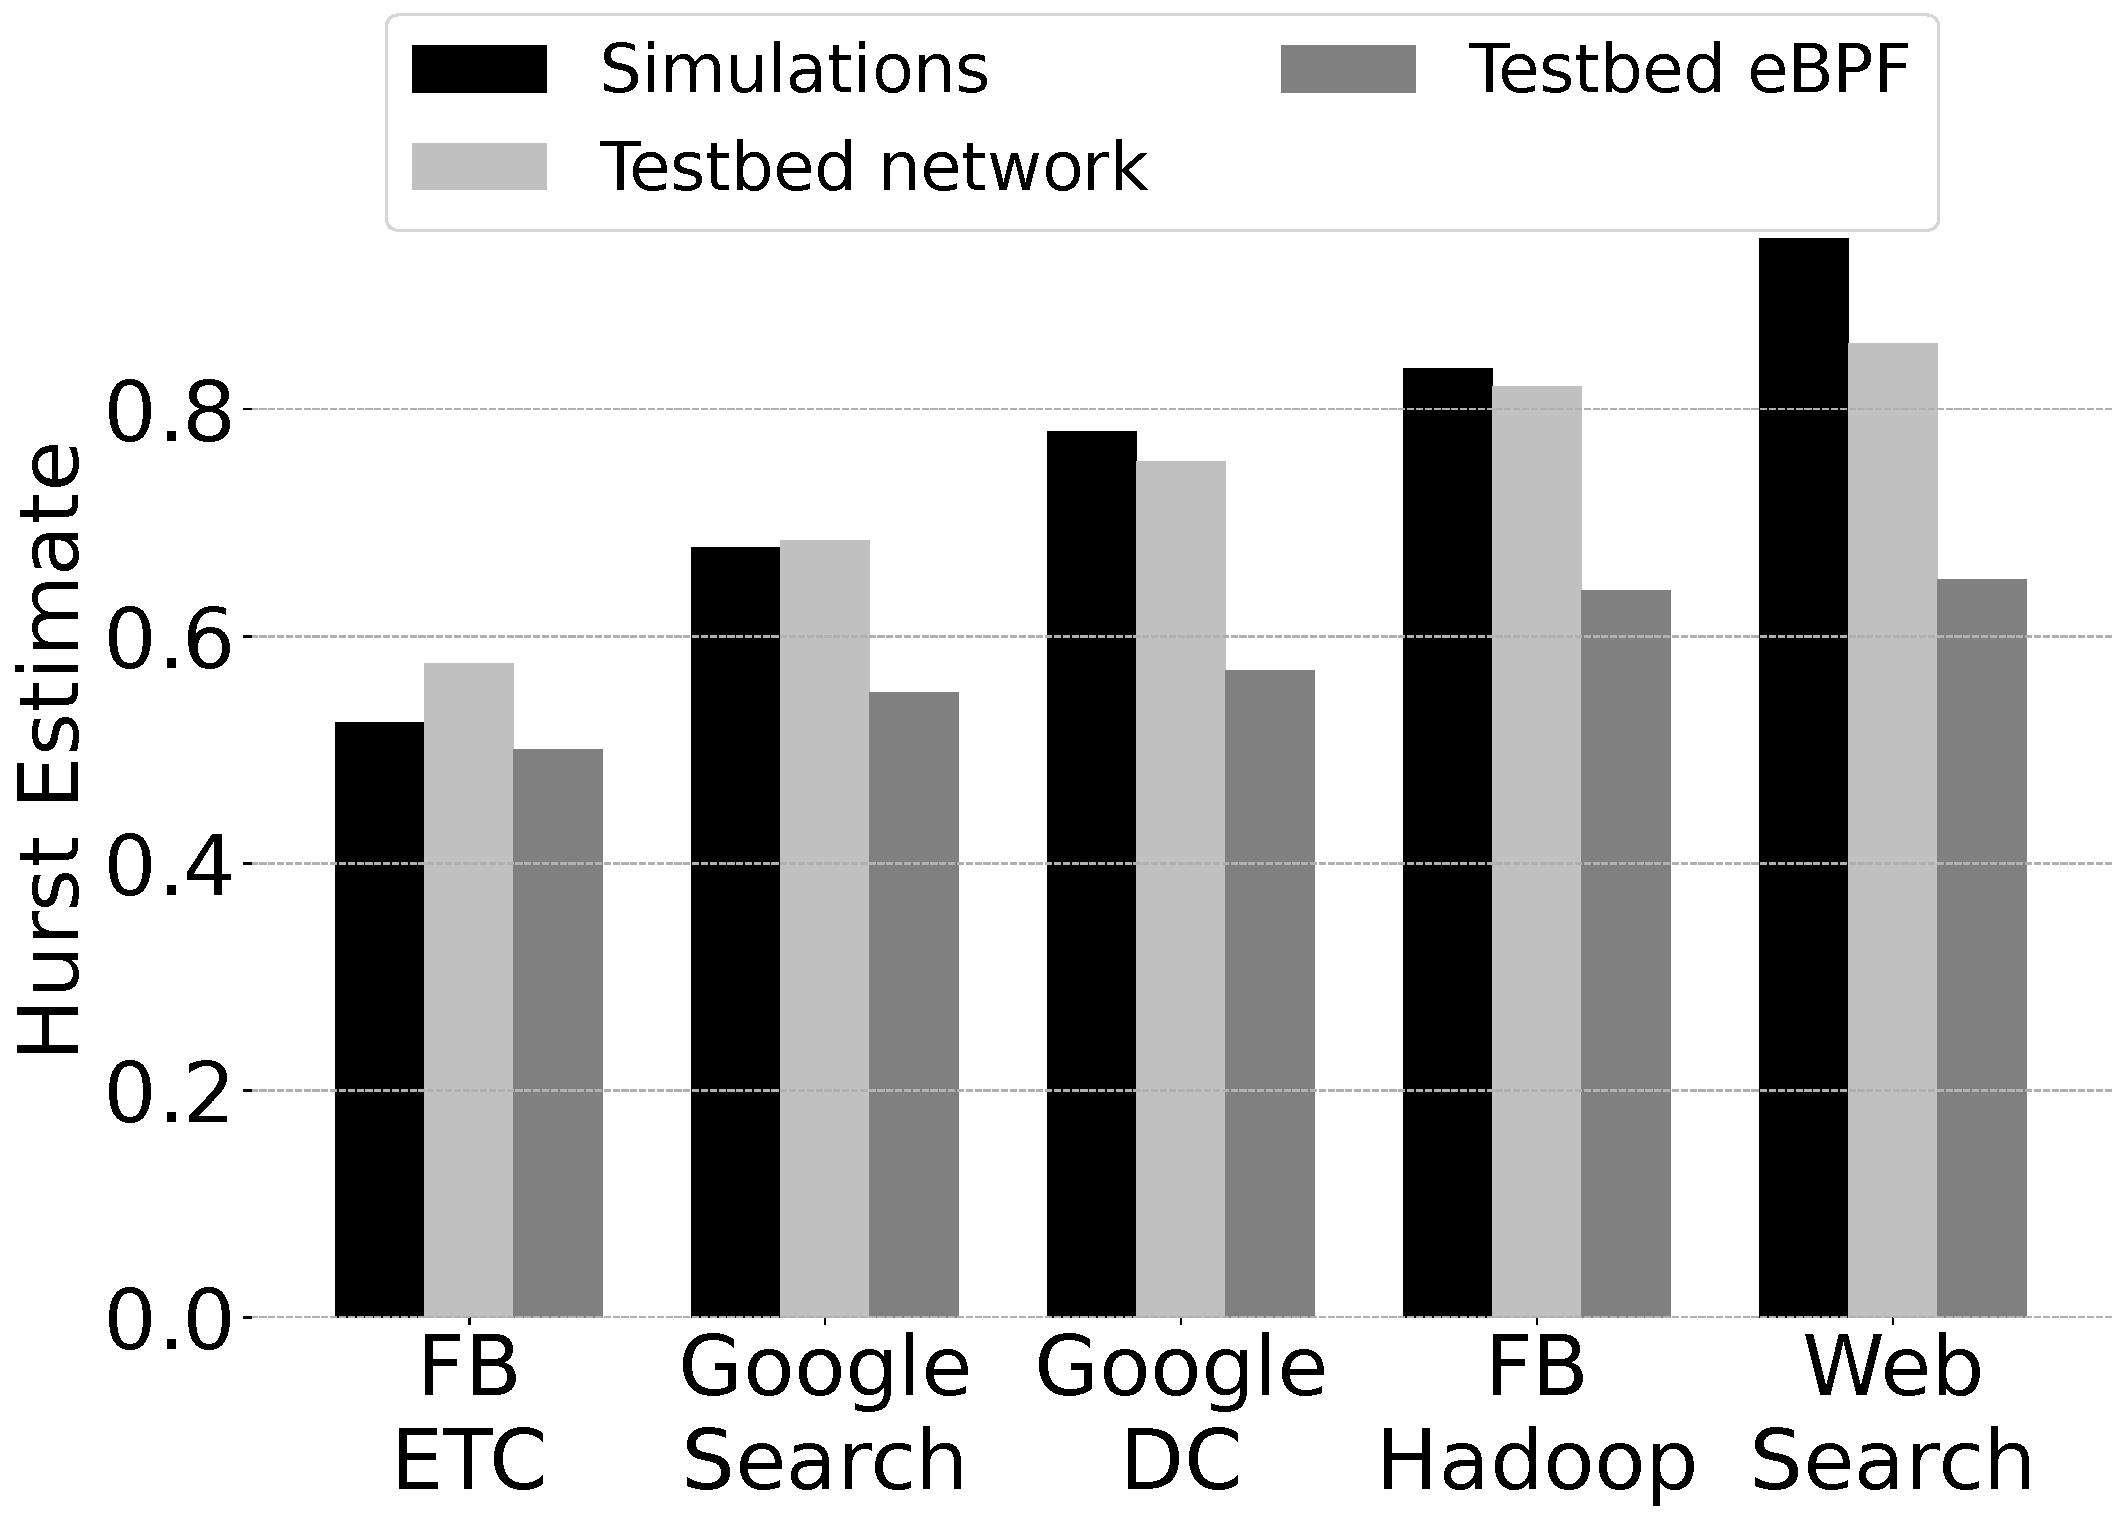
\includegraphics[width=1\linewidth]{figs/w_ebpf_hurst_bar.pdf}
    \caption{Estimated Hurst exponents}
	\label{fig:whurst-ebpf}
\end{subfigure}

    \caption{\small{
    Self-similarity and microburst sizes vary across workloads and between testbed and simulation results. Positioned before the NIC, Valinor-H captures a smoother snapshot of traffic than in-network measurements.
    }}
	\label{fig:traces}
 \vspace{-5mm}
\end{figure}

% \vspace{-2mm}
\subsection{Impact of workloads}
Next, we repeat the above experiments (using both the simulator and the testbed) by replaying the  traces of five classes of workloads from \cite{homa}: (1) Facebook's ETC workload,  (2) Google search workload, (3) Google's aggregated internal data center workload, (4) Facebook's Hadoop workload, (5) DCTCP's web search workload \cite{dctcp}.
Figure \ref{fig:trace-ccdf} shows the flow size distributions of these traces. 
Similar to the previous experiments, in simulations, there exists a direct correlation between the flow size distributions, self-similarity, and the burst lengths (Figure \ref{fig:traces}). In the testbed, however, the difference in burst lengths starts to fade away as host networking components come into play.
%
%Nonetheless, both Valinor-H and Valinor-N are able to capture the differences in traffic burstiness for the five traces of choice. 
We also observe that the scaling behavior varies substantially across different workloads and between the simulated and testbed experiments.
Hurst coefficients are larger for the more heavy-tailed distributions in the network but mostly homogeneous before reaching the driver.
For example, the self-similarity estimates for the ETC workload (p99$^{th}$ flow size = 1.8 KB), the Google DC workload (p99$^{th}$ flow size = 31 KB), and the web search workload (p99$^{th}$ flow size = 27 MB) are 0.57, 0.75, and 0.85, respectively for in-network measurements and 0.50, 0.57, and 0.65, respectively for in-host measurements.
%, all capturing the positive correlation between the workload size and its burstiness.
%The next mission is indeed discovering the role of host networking internals on traffic burstiness. In the following sections, we attempt to provide more insights.

\begin{figure}[t]
\centering
    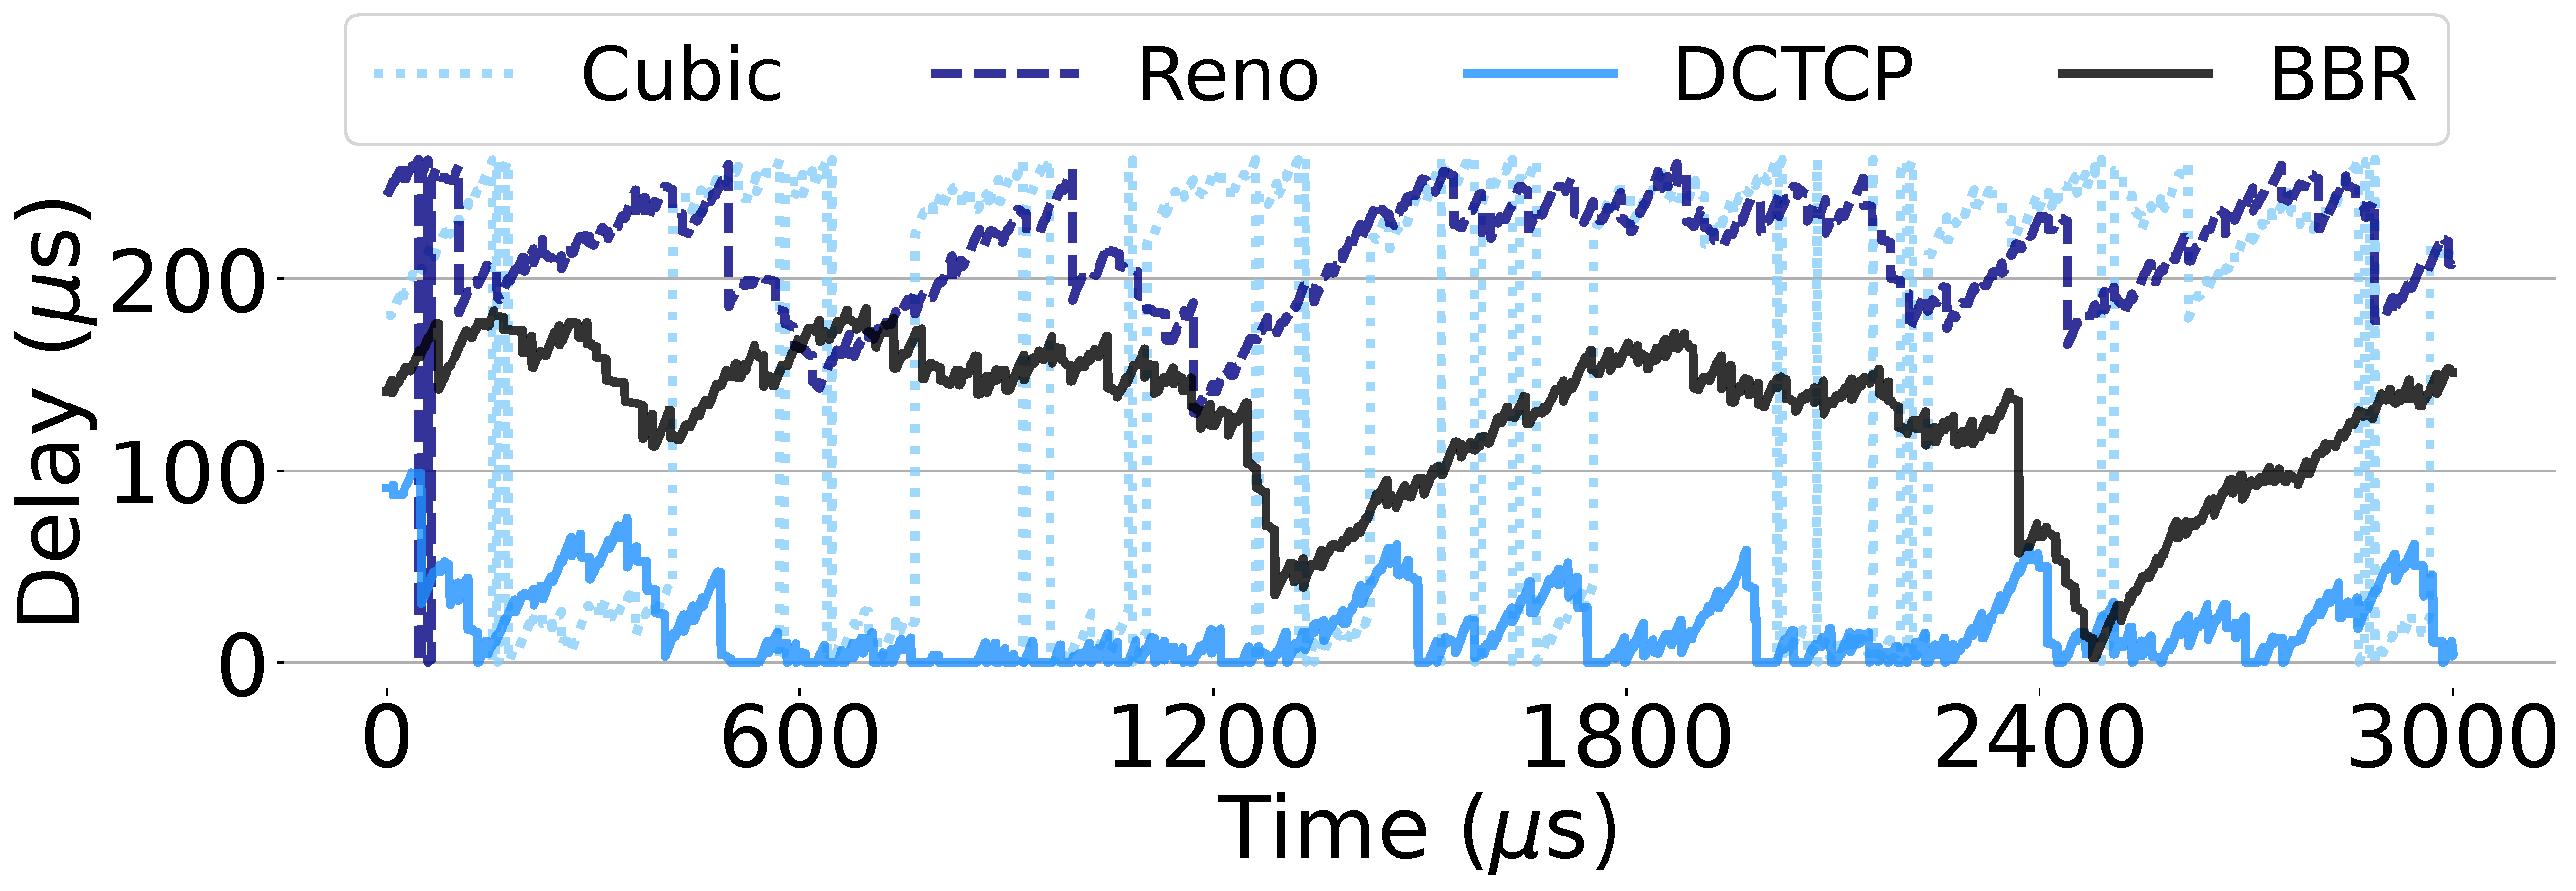
\includegraphics[width=0.8\linewidth]{figs/buffer_size.pdf}
    % \vspace{-6mm}
    \caption{\small{Buffer occupancy under Incast captured by Valinor-N}}
	\label{fig:transport-queue}
 \vspace{-2mm}
\end{figure}
% \vspace{5mm}
\begin{figure}[t]
\centering   
    \vspace{3mm}
    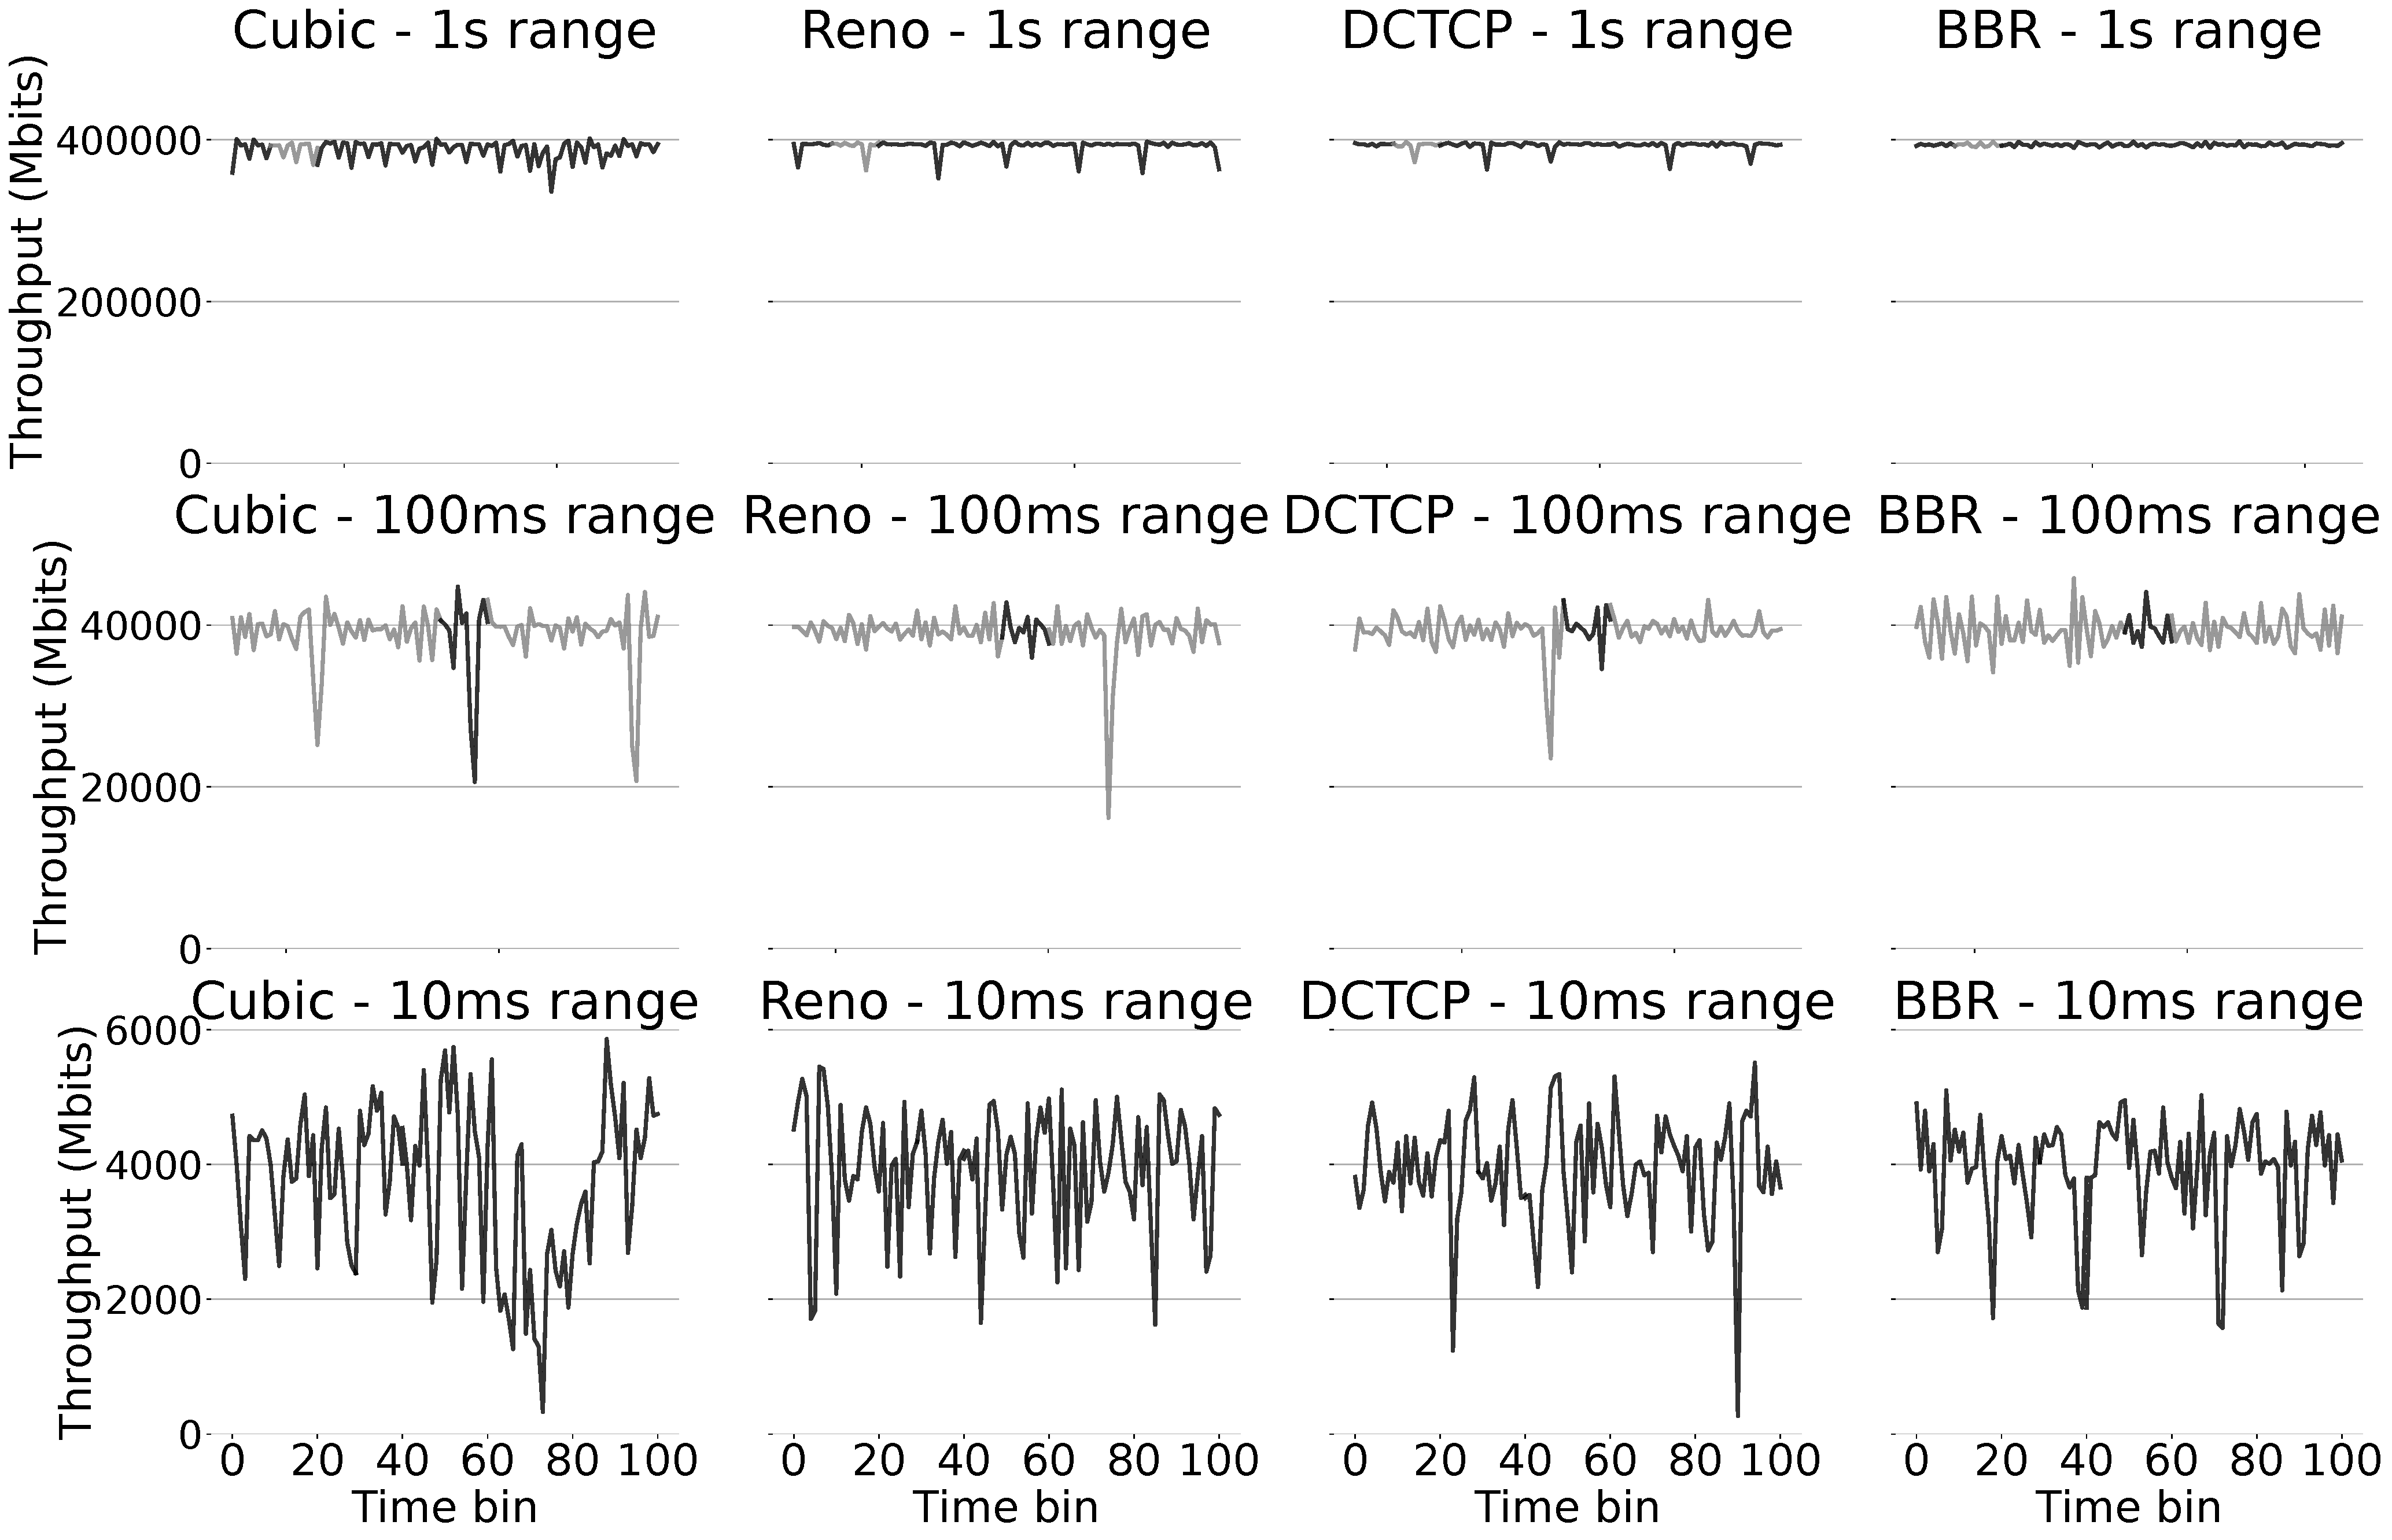
\includegraphics[width=0.85\linewidth]{figs/incast_byte_time_series.pdf}
    % \vspace{-2mm}
    \caption{\small{Timeseries of packet arrivals show that burstiness (at both short and long timescales) varies significantly across transport protocols.}}
	\label{fig:transport-ts}
     \vspace{-2mm}
\end{figure}

\begin{figure}[t]
\begin{minipage}[b]{0.49\textwidth}
    \centering
    	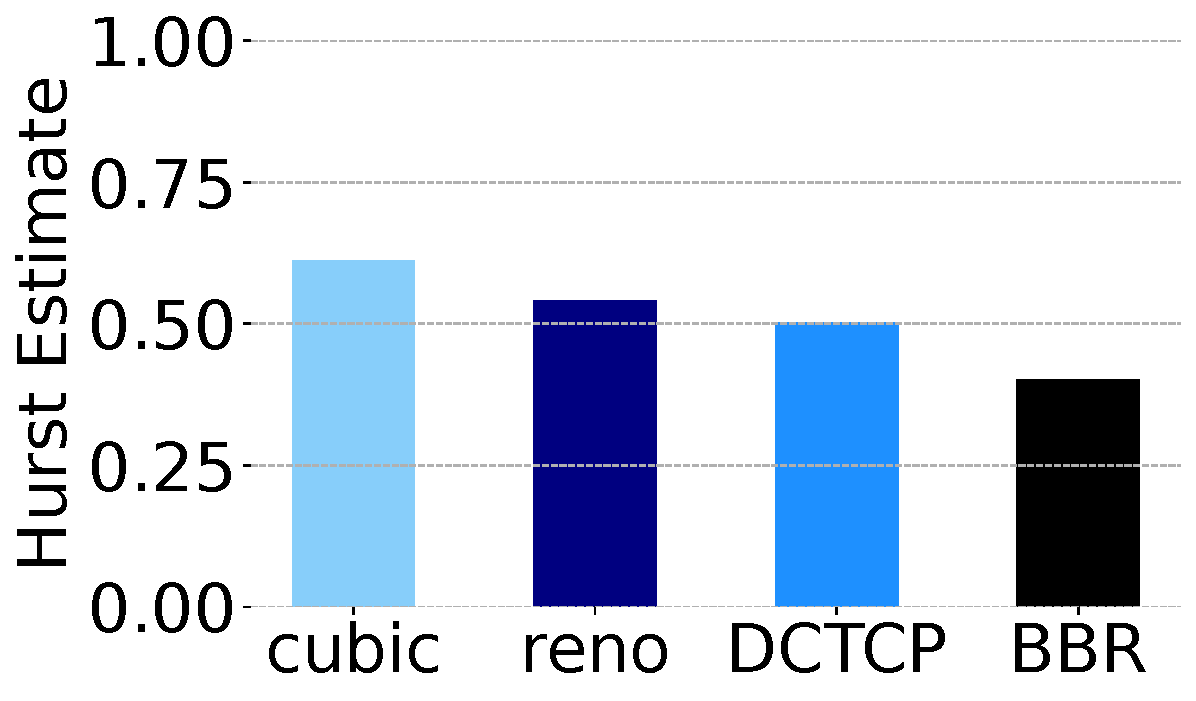
\includegraphics[width=1\linewidth]{figs/transport_hurst_bar.pdf}
    \caption{\small{H estimates for TCP variants suggest lower burstiness under BBR and DCTCP.}}
	\label{fig:transport-hurst}
     \vspace{-2mm}
\end{minipage}
\hspace{2pt}
\begin{minipage}[b]{0.45\textwidth}
    \centering
    	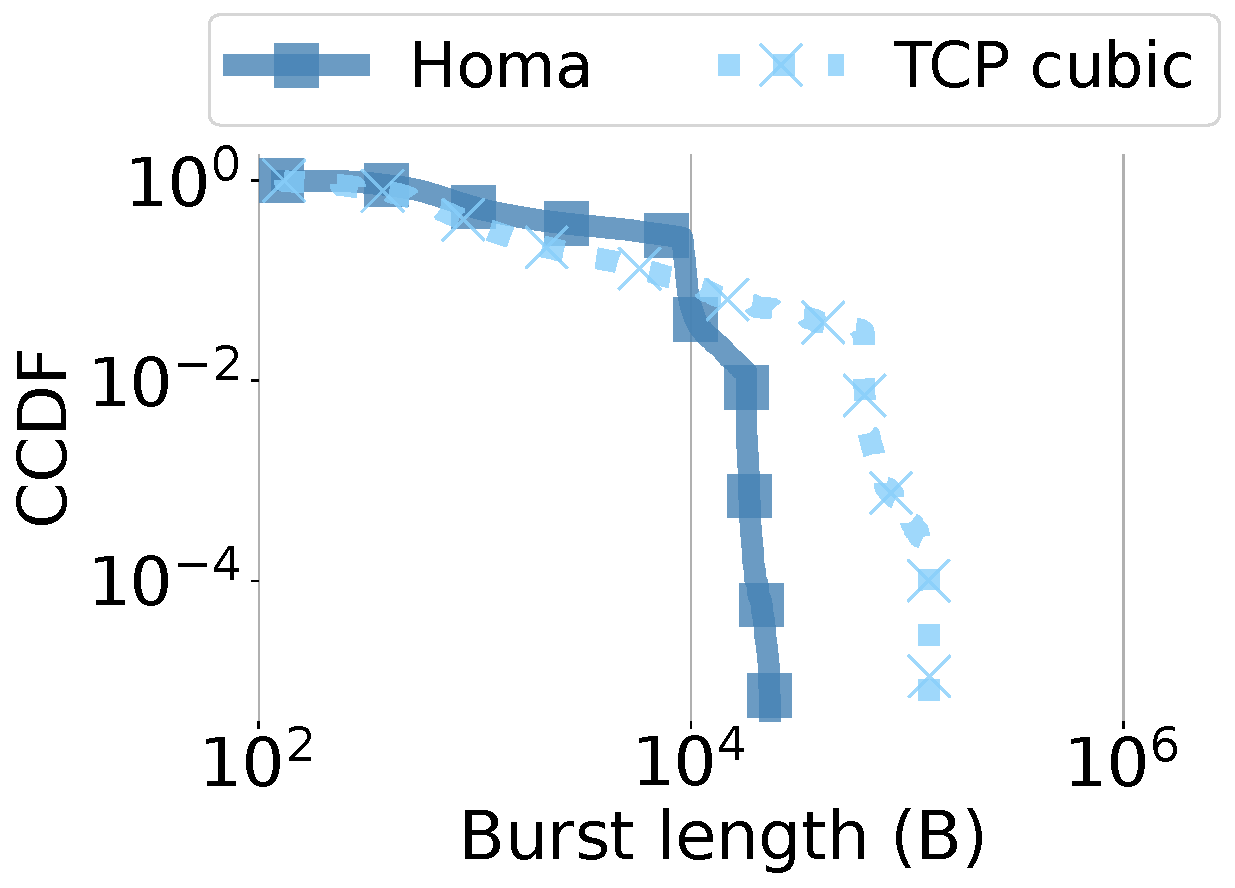
\includegraphics[width=1\linewidth]{figs/homa_ccdf.pdf}
    \caption{\small{A receiver-driven transport, Homa, is less bursty than TCP Cubic.}}
	\label{fig:transport-homa}
     \vspace{-2mm}
     \end{minipage}
\end{figure}



\subsection{Sources and implications of burstiness}
\label{sec:sources}
The previous section shows the aggregate impact of host networking elements on bursts. In this section, we measure the impact of each element, starting with the transport layer and moving to the elements that operate \emph{below} the TCP/IP stack (e.g., qdiscs) and \emph{in parallel} to it (e.g., the process scheduler).
%To find the culprits behind traffic burstiness, we direct our focus toward layers of network stack processing. Starting with the transport protocols, we investigate each layer separately by trying different configurations while keeping the rest of the systems fixed.




\subsubsection{Transports and congestion control}
Starting with transports, we evaluate four TCP congestion control variants under a mixture of background traffic and a small-scale incast traffic pattern where two sender machines target one receiver. The background traffic consists of two \textit{iperf} flows each taking 18Gbps of bottleneck link bandwidth. The incast traffic follows the map-reduce workload size distribution. For this experiment only, we run both the workload generators and the applications outside the container environment. Figure \ref{fig:transport-queue} shows how TCP Cubic \cite{cubic}, TCP Reno, DCTCP \cite{dctcp}, and BBR \cite{bbr} react to queue buildups in the network. 
Compared to Reno, TCP Cubic (the default congestion control setting in recent versions of Linux kernels) uses a more aggressive function for increasing its congestion window upon receiving acknowledgments. Therefore, it experiences larger queueing oscillations than Reno. BBR uses round-trip times to adjust its transmission window and varies its pacing rate to keep the in-flight bytes near its estimated bandwidth-delay product. Thus, it experiences a more steady queueing behavior while trying to keep the buffer half full. Finally, DCTCP uses explicit congestion notifications from switches to maintain consistently low queuing.

Figure \ref{fig:transport-ts} presents the throughput timeseries of the four congestion control variants at different timescales followed by their Hurst exponent estimates in Figure \ref{fig:transport-hurst}.
With the help of pacing and RTT estimations, BBR is able to maintain a steady throughput and a non-bursty traffic shape, reflected by $H = 0.40$.
On the other hand, Cubic's less conservative transmissions incur a self-similarity estimate of 0.60.

Finally, we deploy Homa's kernel module \cite{homa} as a representative implementation of receiver-driven transports in the Linux kernel. In receiver-driven transports, the destination initiates more packets by issuing \textit{grant} control packets for the sending host. In our setup, Homa sends the first 90 KB of each flow unscheduled as an attempt to initiate the communication and retrieve the path's congestion status. The following packets are then scheduled using grants. 
Due to its limited implementation scope, the Homa module is not able to achieve line rate performance. Therefore, we limit our observation to the map-reduce workload tuned down to 6 Gbps offered load. 
Figure \ref{fig:transport-homa} presents the burst lengths for Homa and TCP Cubic as observed by Valinor-H eBPF framework. We observe that the p99 burst length under Homa is 9$\times$ lower than Cubic which might reflect two facts. First, unlike Cubic which sends up to 64 KB long data chunks, Homa's prepared \textit{sk\_buff} chunks are mostly as large as its MTU (9 KB in this experiment). This is also due to the fact that Homa kernel module is not making use of TSO because of certain Intel NIC limitations. Secondly, Homa uses pacing to keep the NIC fully saturated in its Linux implementation which further controls the spacing between its transmissions \cite{homa-impl}.
%
Combined, these factors result in Homa's less bursty behavior compared to TCP Cubic, not just at small timescales (Figure \ref{fig:transport-homa}) but also at large timescales ($H=0.54$ for Homa \emph{vs.} 0.62 for Cubic). However, we suspect a different behavior from Homa on different setups that can make use of NIC offloading.



\subsubsection{Software switching}
\label{sec:qdisc}
Linux leverages queueing disciplines (\textit{qdiscs}) to enforce scheduling among segments originating from different applications in the system. If generic segmentation offload is not in use, \textit{qdiscs} are the last software components to decide the order of data entities on NIC's FIFO rings.
We study five representative queueing disciplines implemented in Linux:
\\
\textbf{1) Fair queue (fq)} is the default scheduler in recent Linux kernels and is mainly used to enforce pacing on a per-flow (per socket) basis. The appropriate pace among flows is either explicitly enforced via socket options, or is determined by the TCP congestion control (e.g., BBR). By default, \textit{fq} uses deficit round-robin with a default quantum of 3028 bytes to drain flow queues, with an initial quantum equalling TCP's initial 10-packet window.
% \\
% \textbf{2) CHOKe (CHOose and Keep for responsive flows, CHOose and Kill for unresponsive flows)} is an Active Queue Management (AQM) algorithm aimed at preventing bufferbloat \cite{bufferbloat}. CHOKe is a variant of the Random Early Drop (RED) scheme and uses a randomized algorithm to enforce early drops on flows that monopolize the queue.
\\
\textbf{2) fq\_CoDel.} The controlled delay (CoDel) algorithm, combined with fair queue, enforces CoDel on per-flow sub-queues. CoDel, a more recent AQM algorithm, uses packet sojourn time inside each flow queue to detect slow flows and prevents the queueing delay to exceed a user-specified target by dropping excess traffic.
\\
\textbf{3) Stochastic Fair Queueing (SFQ)} extends flow-queuing with random-early marking/drop semantics with small default queue sizing to control the queueing delay. Similar to \textit{fq}, it uses round-robin scheduling on per-flow sub-queues. SFQ uses a default deficit of one MTU.
\\
\textbf{4) pfifo\_fast} is a First-In First-Out priority queue. Higher priority packets are distinguished by their Type of Service (TOS) fields in IP headers which are set by upper layers.
\\
\textbf{5) Heavy Hitter Filter (HHF)} attempts to identify and separate short flows from heavy hitters to prevent head-of-the-line blocking and increased delays for latency-sensitive flows. Such flows are given a higher deficit compared to heavy hitters in each transmission round.

We study qdiscs under three scenarios: First, to see the actual contribution of qdiscs to the traffic shape, we disable segmentation offload and serialization offload and limit the number of the transmit rings to one (single-queue). Segmentation is the process of breaking large \textit{sk\_buffs} into MTU-sized segments and is usually deferred to the last processing stages to reduce CPU utilization and improve flow performance. Segmentation offload can either be performed in the hardware (TCP Segmentation Offload or TSO) or just before passing the data to the hardware (Generic Segmentation Offload or GSO). Additionally, in a multi-queue architecture, the network stack communicates to the NIC via separate ring buffers pinned to each CPU core to reduce inter-core communication overheads and improve throughput. When enabled, a (reportedly, round-robin \cite{titan}) packet scheduler in the hardware will decide the order in which packets are drained from ring buffers.

Initially, we run 1000 Iperf instances spread across 200 containers, simulating the map-reduce workload on the single-queue server without offloading. Figure \ref{fig:qdisc} demonstrates how, \emph{in isolation}, per-flow queuing can significantly shorten the size of egress bursts. Techniques such \textit{pfifo\_fast}, and HHF use one large buffer containing packets from all egress flows, allowing multiple data segments of one flow to be enqueued simultaneously. On the other hand, per-flow queueing allows the scheduler to interleave among packets of different flows, primarily to maintain fairness and prevent head-of-the-line blocking \cite{backdraft}.

To verify the impact of round-robin scheduling on blunting bursts, we repeat the same experiment with \textit{fq} qdisc, increasing the per-flow deficit from one MTU (1514 bytes) to 16 MTUs, and observe a linear correlation between fq deficits and burst lengths. For example, the 90$^{th}$ percentile of burst lengths under a deficit of 16 packets is increased to 25 KB from 13 KB under that of 8 MTUs (92\% increase). 
% This also explains why SFQ qdiscs is the least bursty in the previous experiment.

\begin{figure*}[t]
\centering
\begin{subfigure}[t]{0.32\linewidth}
    \centering
    	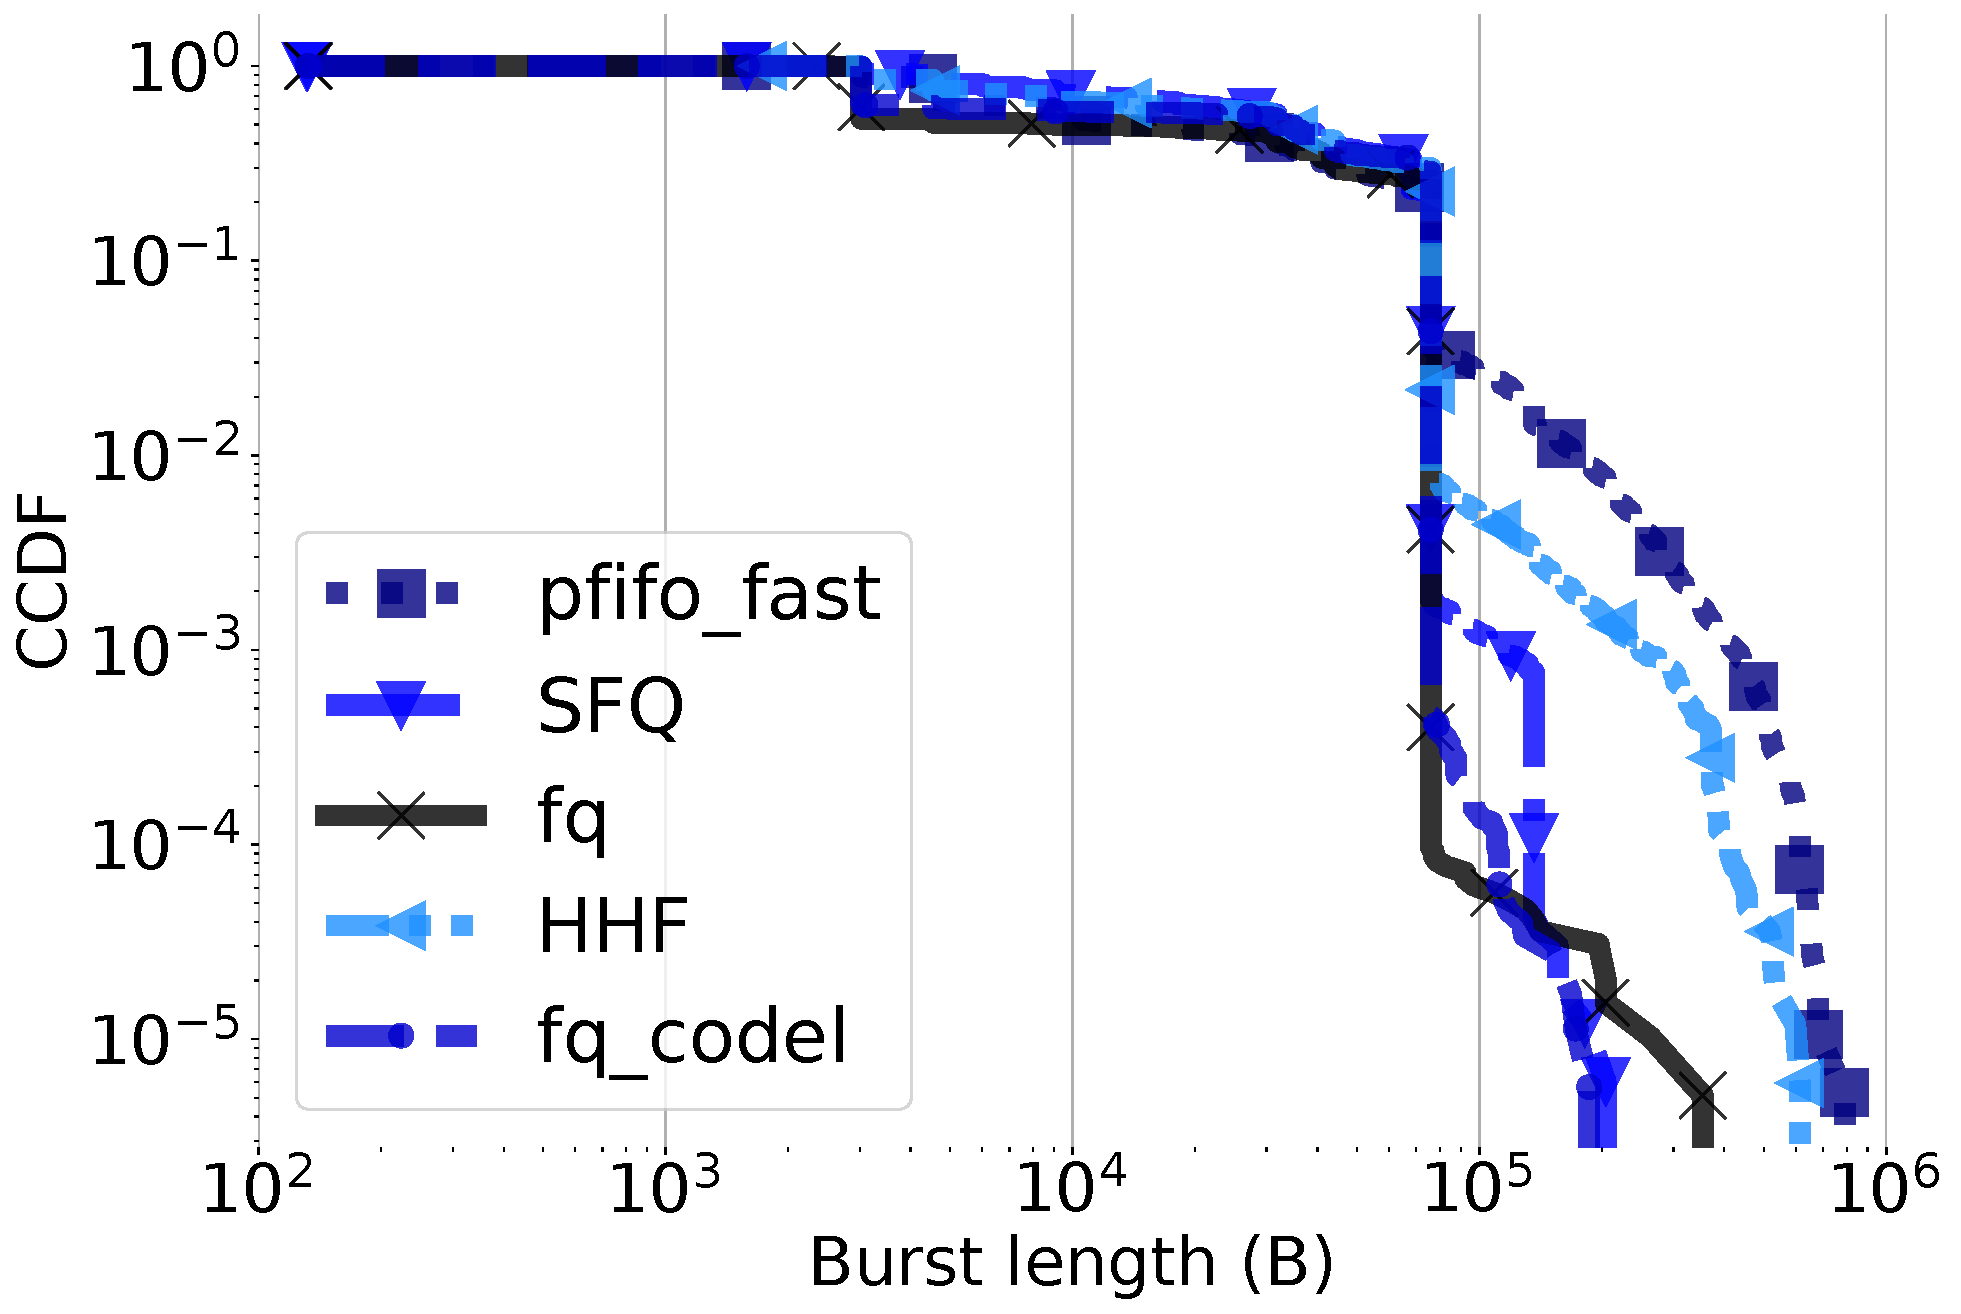
\includegraphics[width=1\linewidth]{figs/26_4.pdf}
    \caption{SQ w/out Offloading}
	\label{fig:qdisc}
\end{subfigure}
\begin{subfigure}[t]{0.32\linewidth}
    \centering
    	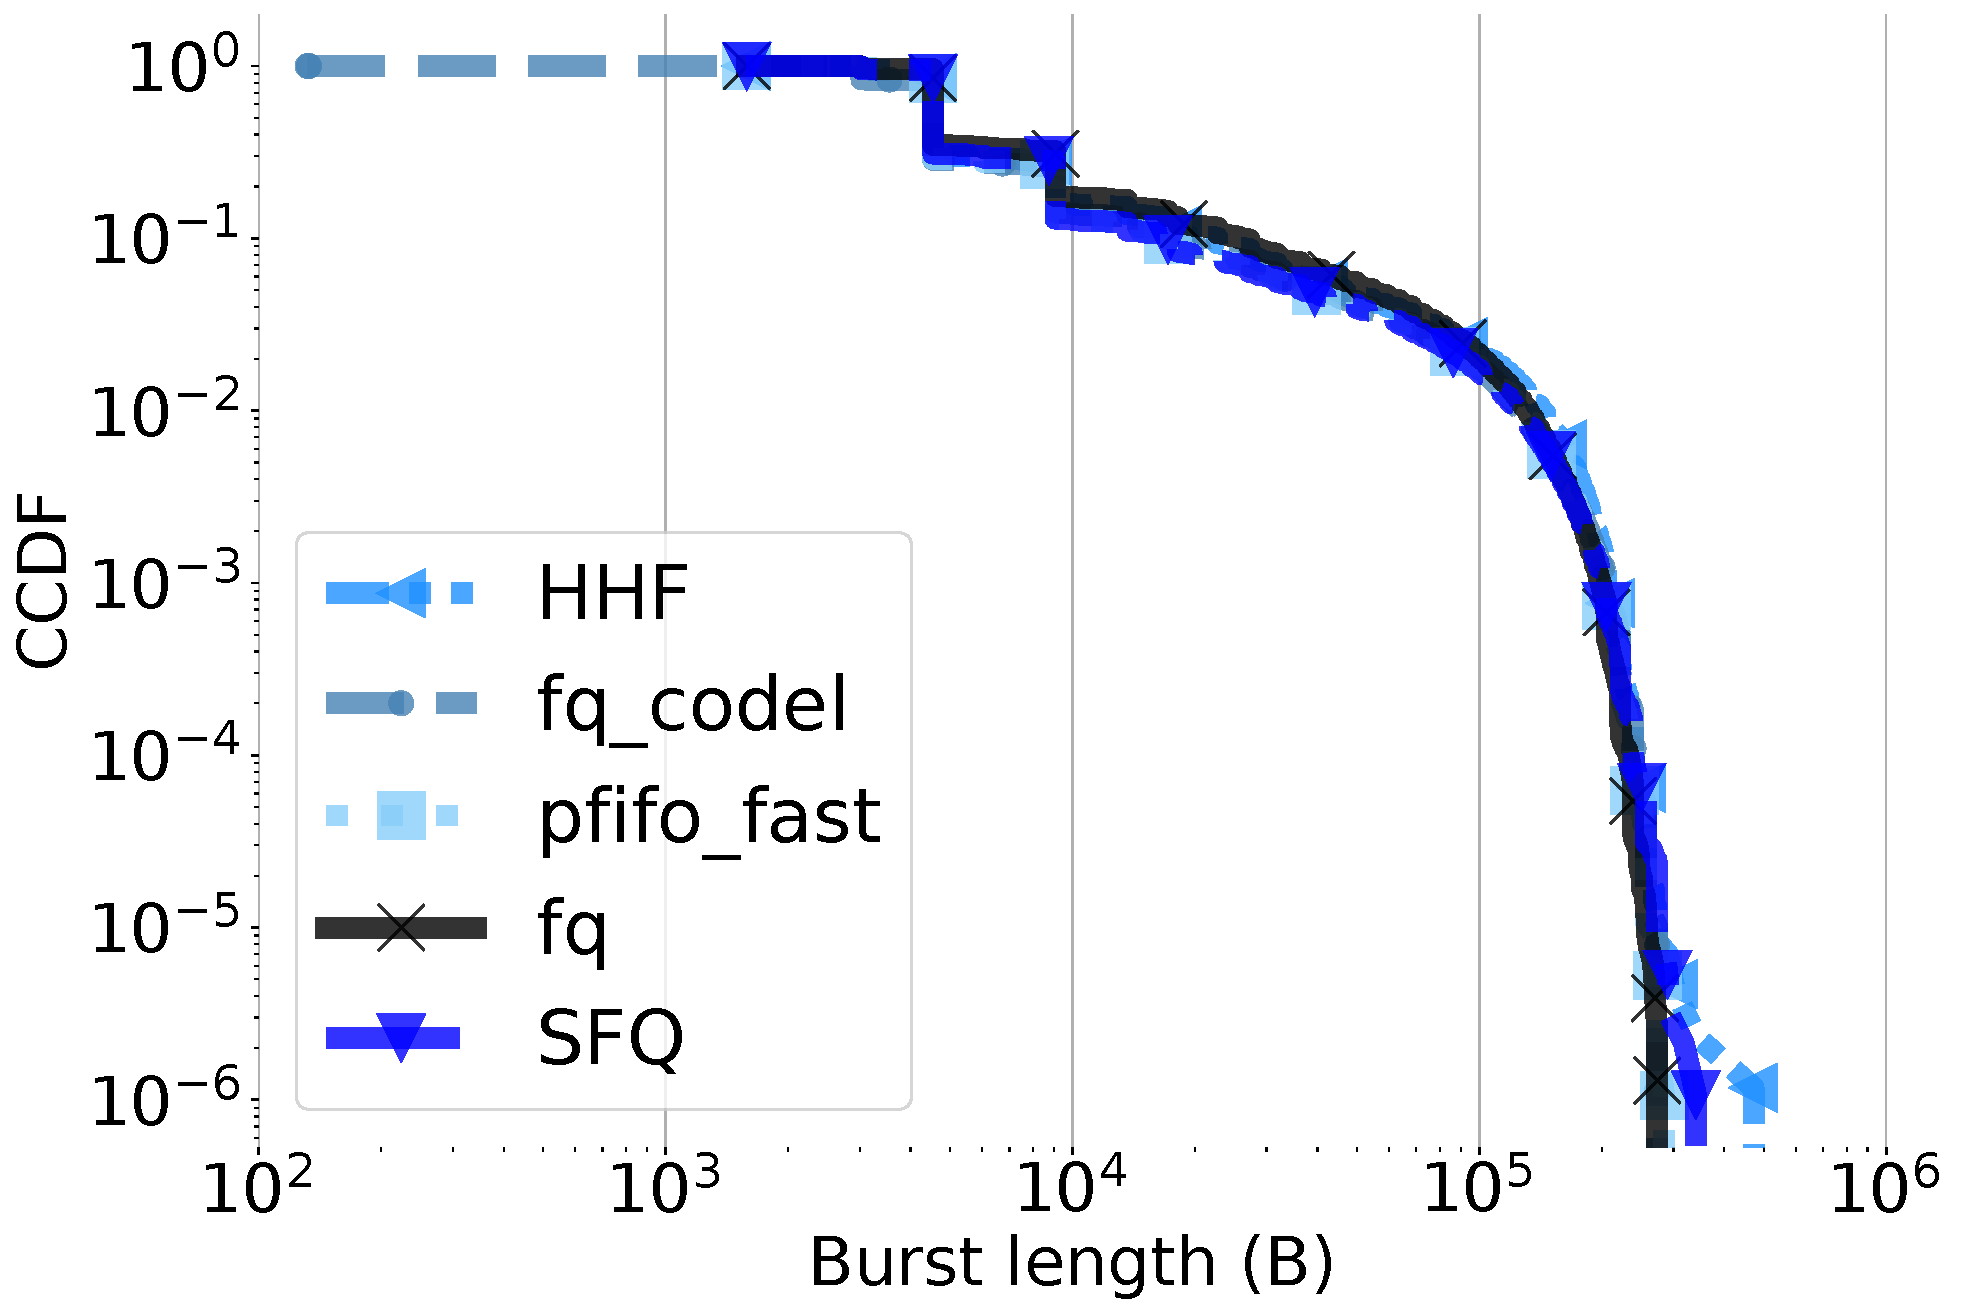
\includegraphics[width=1\linewidth]{figs/26_6_fig.pdf}
    \caption{SQ w/ Offloading}
	\label{fig:qdisc_tso}
\end{subfigure}
\begin{subfigure}[t]{0.32\linewidth}
    \centering
    	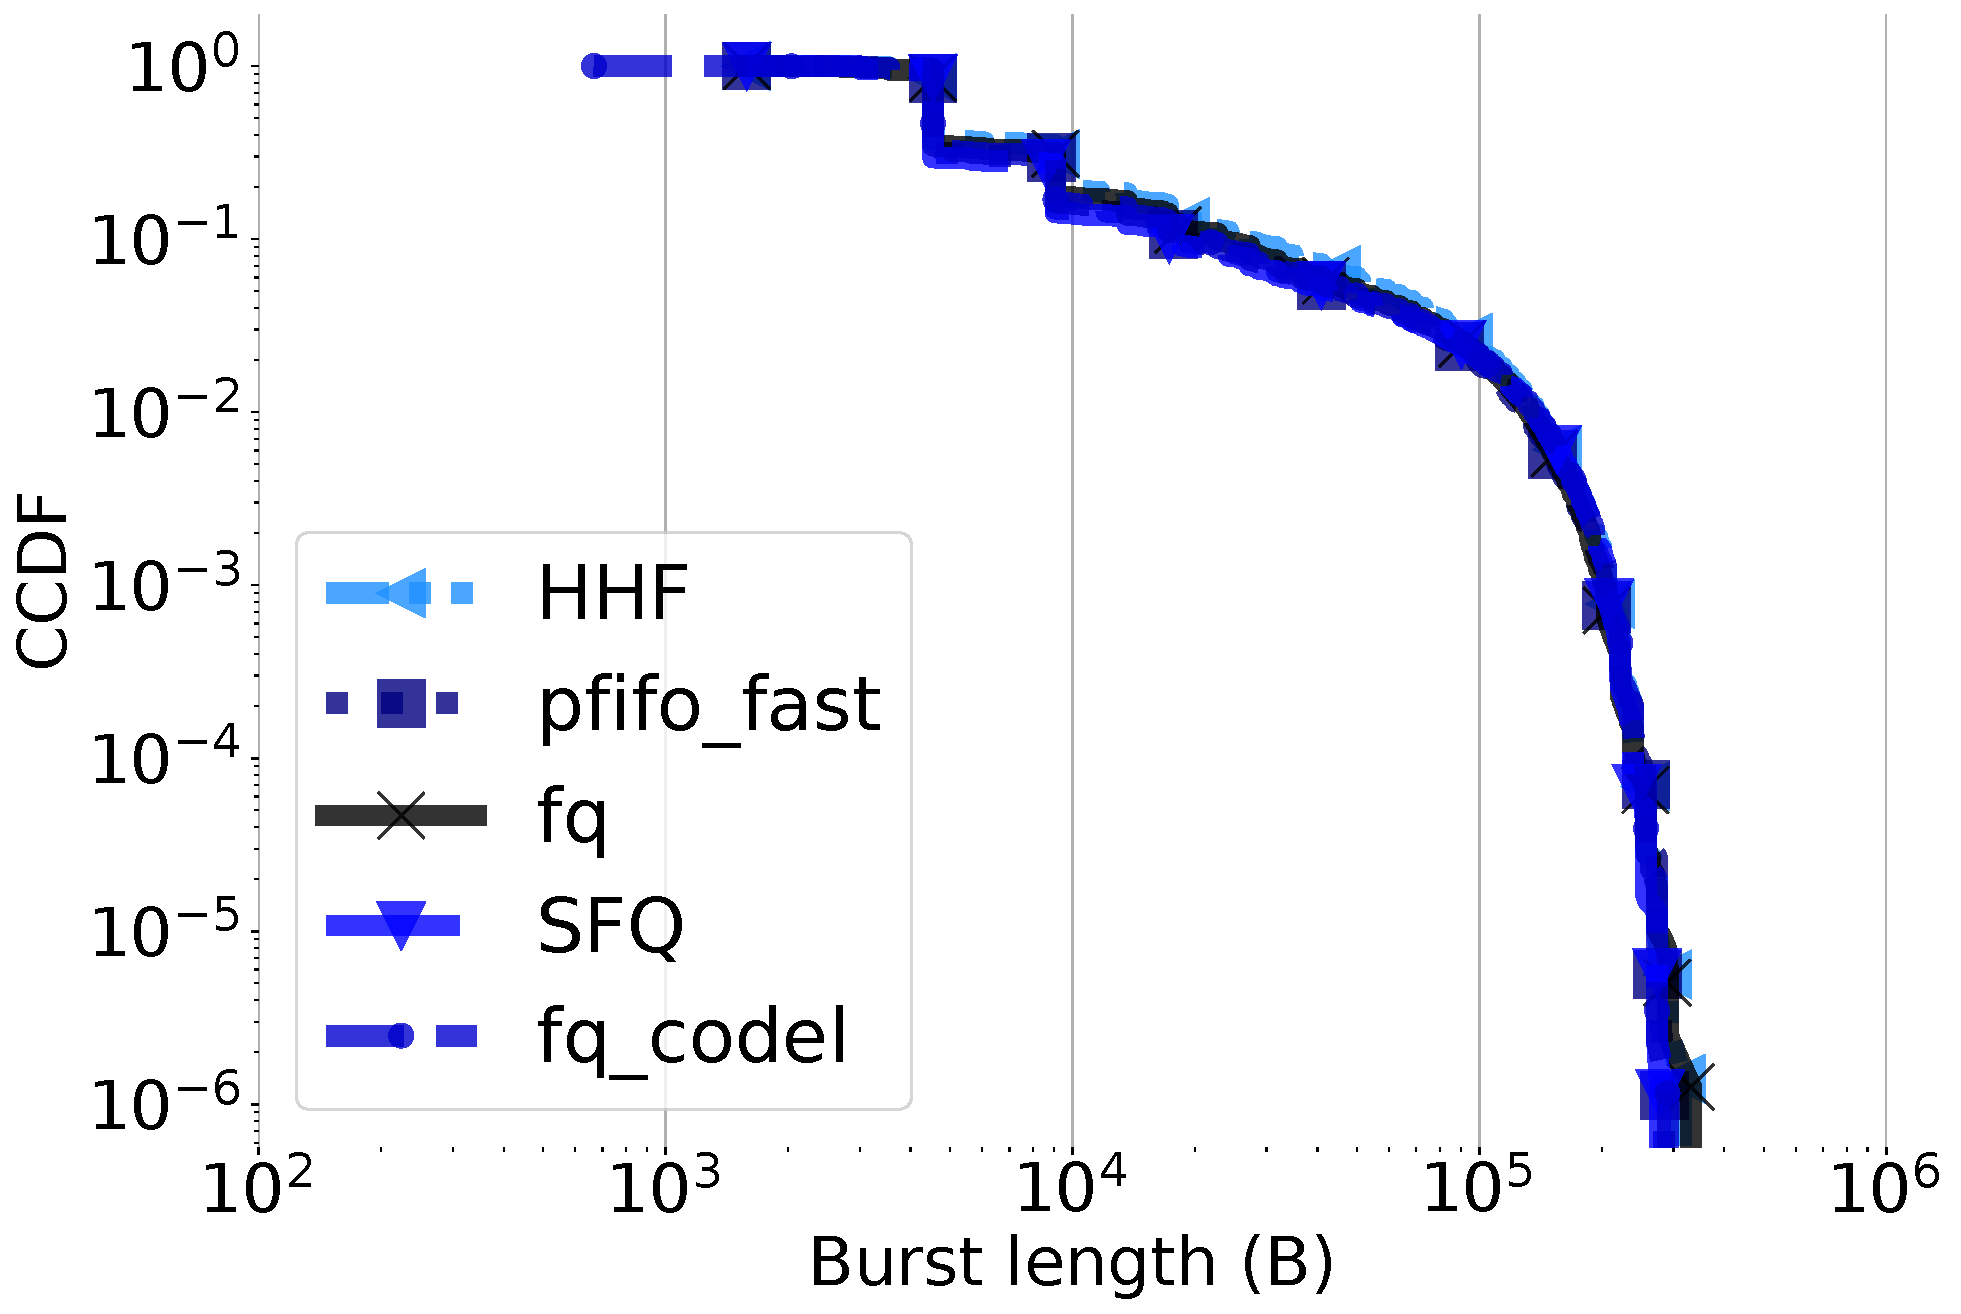
\includegraphics[width=1\linewidth]{figs/26_2.pdf}
    % 	\vspace{5mm}
    \caption{MQ w/ Offloading}
	\label{fig:qdisc_mq}
\end{subfigure}

\vspace{-2mm}
\caption{\small{Both Multi-queueing (MQ) and TCP segmentation offload compromise the intended shape of software packet scheduling.}}
\vspace{-2mm}
\end{figure*}

While qdisc is the last layer to perform packet scheduling in the software, the traffic ultimately often passes through segmentation offloading and NIC scheduling before reaching the wire. Is the impact of qdiscs on the wire preserved \emph{after the interaction} with these lower layers?
To investigate, we enable all the offloading features and perform our measurements again. Figure \ref{fig:qdisc_tso} demonstrates the impact of offloading segmentation and serialization on lengthening the egress bursts. SQ represents Single Queue NICs while MQ represents Multi-queueing combined with a layer of round-robin scheduling at the NIC. With TSO at work, qdiscs no longer serve packets. Instead, they schedule between dynamically sized \textit{sk\_buffs}. Hardware offloading then helps increase the throughput by nearly 50\% for all cases while moving the buffering to the hardware where large segments are broken into MTU-sized packets and sent on the wire. This significantly undermines qdisc's decisions on shaping the traffic. With offloading in action, the median burst sizes for \textit{fq}, \textit{fq\_codel}, and \textit{pfifo\_fast} are, 132 kB, 127 kB, and 127 kB, respectively. While without offloading, these systems experienced a median burst length of 76 kB, 76 kB, and 172 kB\footnote{pfifo\_fast combined with offloading can exacerbate burstiness as both layers are prone to creating large, uncontrolled bursts.}, respectively.

\begin{figure}[t]
\centering
\begin{subfigure}[t]{0.75\linewidth}
    \centering
    	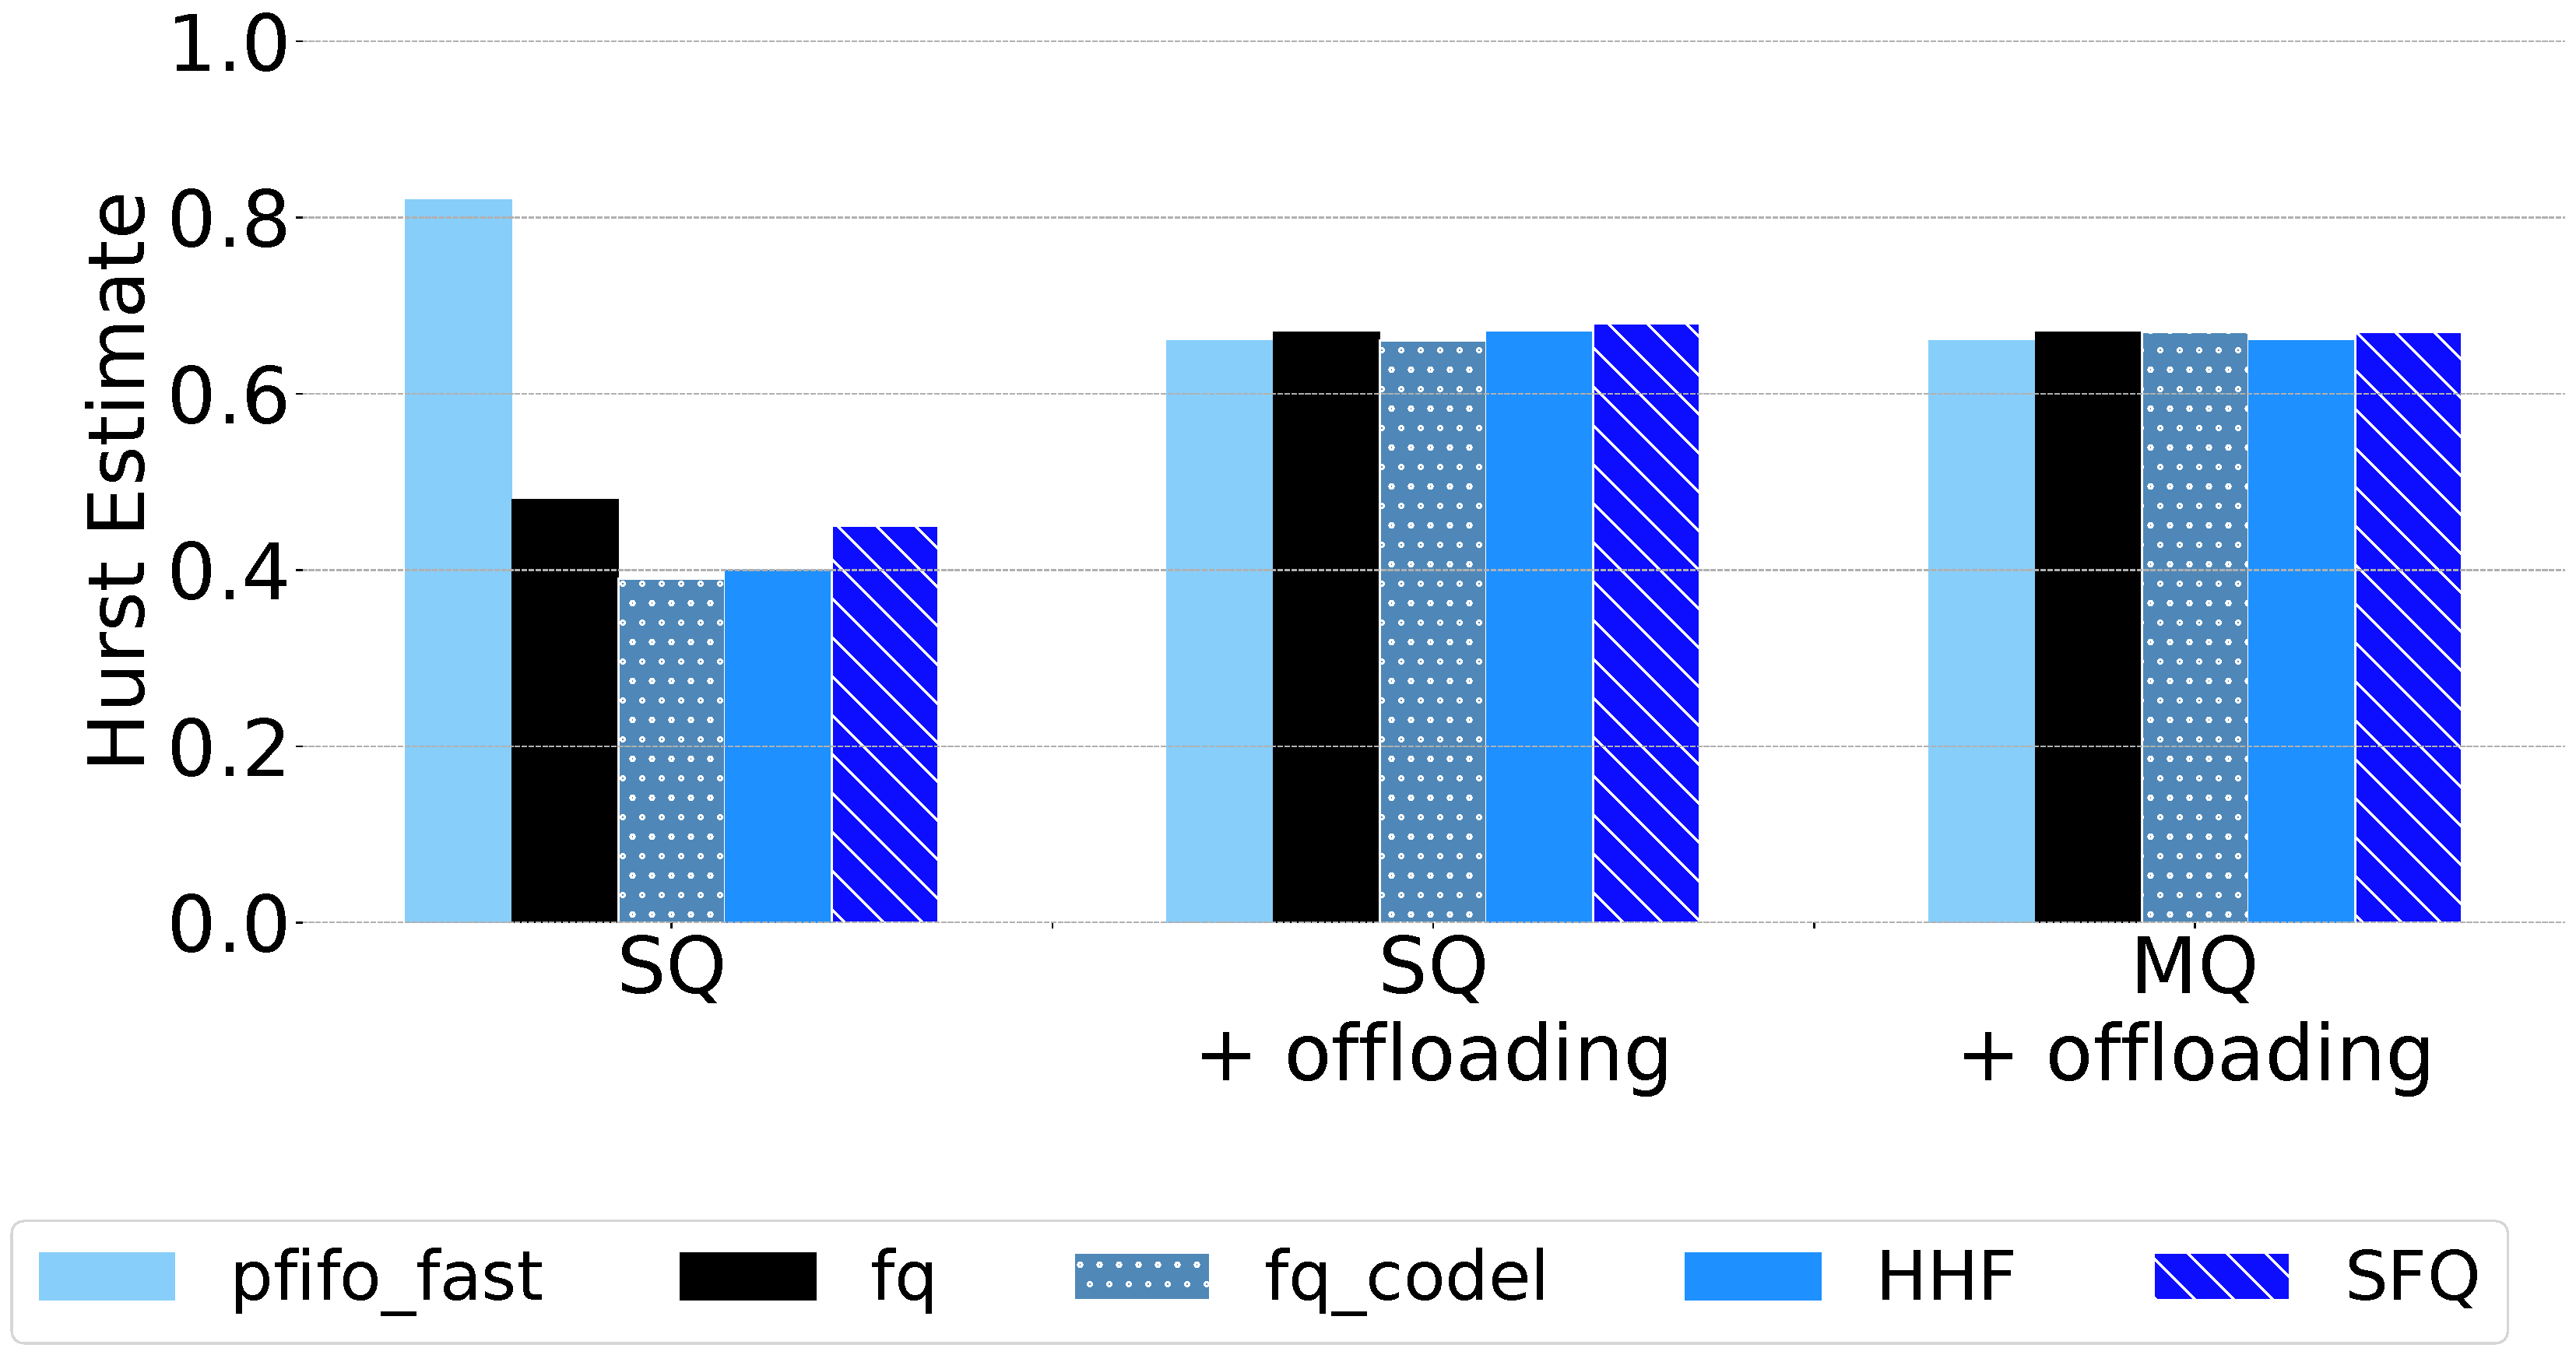
\includegraphics[width=1\linewidth]{figs/nic_hurst_bar.pdf}
    % 	\vspace{5mm}
    % \caption{\small{\textbf{Hurst estimates}}}
\end{subfigure}
\vspace{-2mm}
\caption{\small{Hurst estimates for different Linux packet schedulers.}}
	\label{fig:nic_hurst_bar}
\vspace{-2mm}
\end{figure}

To further ruffle the output of qdiscs, we enable the default multi-ring root qdisc which assigns a separate qdisc instance to each CPU core and enables the NIC scheduler to perform last-level scheduling on transmit rings (multi-queue architecture). Figure \ref{fig:qdisc_mq} presents the outcome. \textit{With NIC scheduling and segmentation offloading at work, the shape of the qdisc's outgoing traffic is barely preserved on the wire.} That is because, NICs are equipped with internal round-robin schedulers to drain the software rings, further reducing the chances of creating long bursts. Finally, Figure \ref{fig:nic_hurst_bar} demonstrates the estimated Hurst exponents for the three scenarios. Without segmentation offloading, the degree of burstiness is considerably reduced (H < 0.5) for all but one case. Only \textit{pfifo\_fast} which does not offer any form of fair queueing suffers from heavier burstiness ($H=0.8$) under the single-queue scenario.
\\
\textbf{Implications of disabling offloading and multi-ring scheduling.}
Apart from burstiness, both offloading and NIC scheduling have a profound impact on flow performance metrics. Our measurements demonstrate that disabling TCP segmentation offload for a workload consisting of 1000 same-size flows results in 71\% decline in median flow throughput, 46\% increase in median packet RTTs, and 3$\times$ increase in sender CPU utilization. Therefore, disabling offloading, in order to enable software control is not always a viable option. 
Multi-queue NICs are also considered a quick solution with potential side effects. While enabling multi-queue reduces resource contention, they can increase response times and are usually fixed-function \cite{titan}.

% \begin{tcolorbox}

% \textbf{Finding x}
% Single-queue disciplines demonstrate uncontrolled burstiness in the absence of NIC scheduling and offloading. With offloading and multi-ring scheduling enabled, qdiscs can barely impact the shape of egress traffic.
% \end{tcolorbox}

% \begin{tcolorbox}

% \textbf{Finding x}
% Scheduling disciplines that use deficit round-robin with a large quantum are prone to producing longer $\mu$bursts.
% \end{tcolorbox}

\begin{figure}
    \centering
    \begin{subfigure}[t]{0.40\linewidth}
    \centering
    	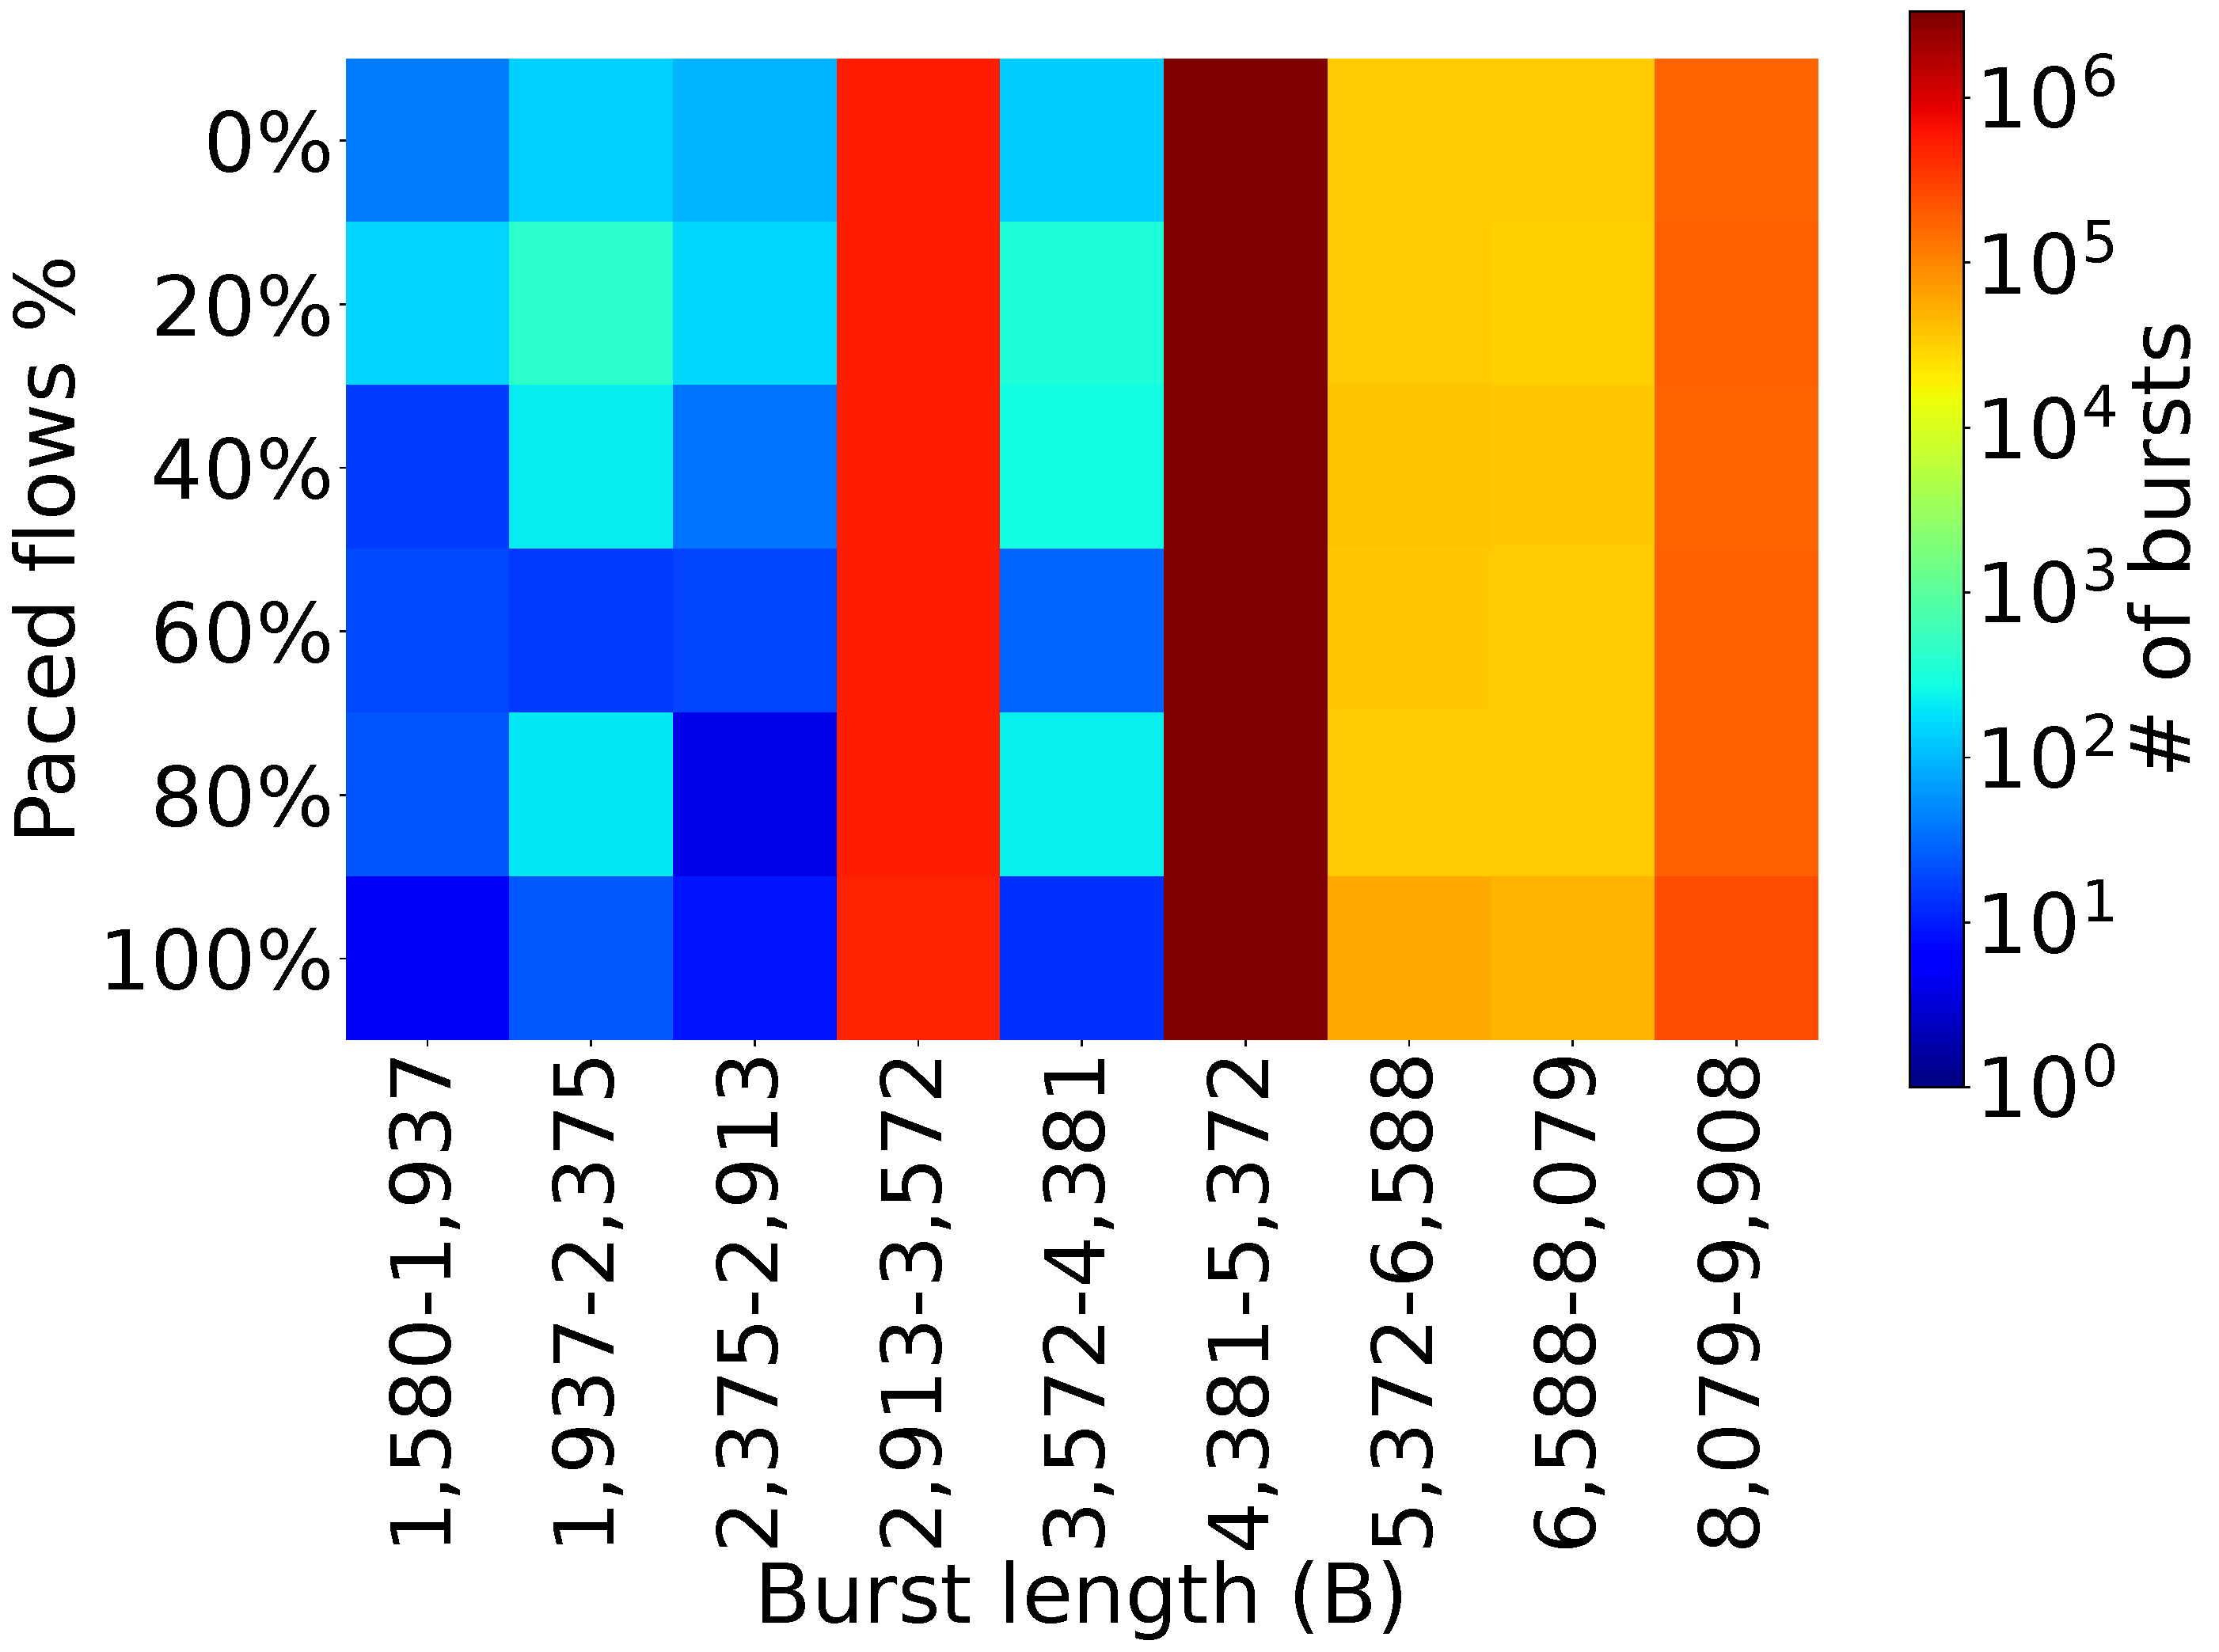
\includegraphics[width=1\linewidth]{figs/pacing1.pdf}
    	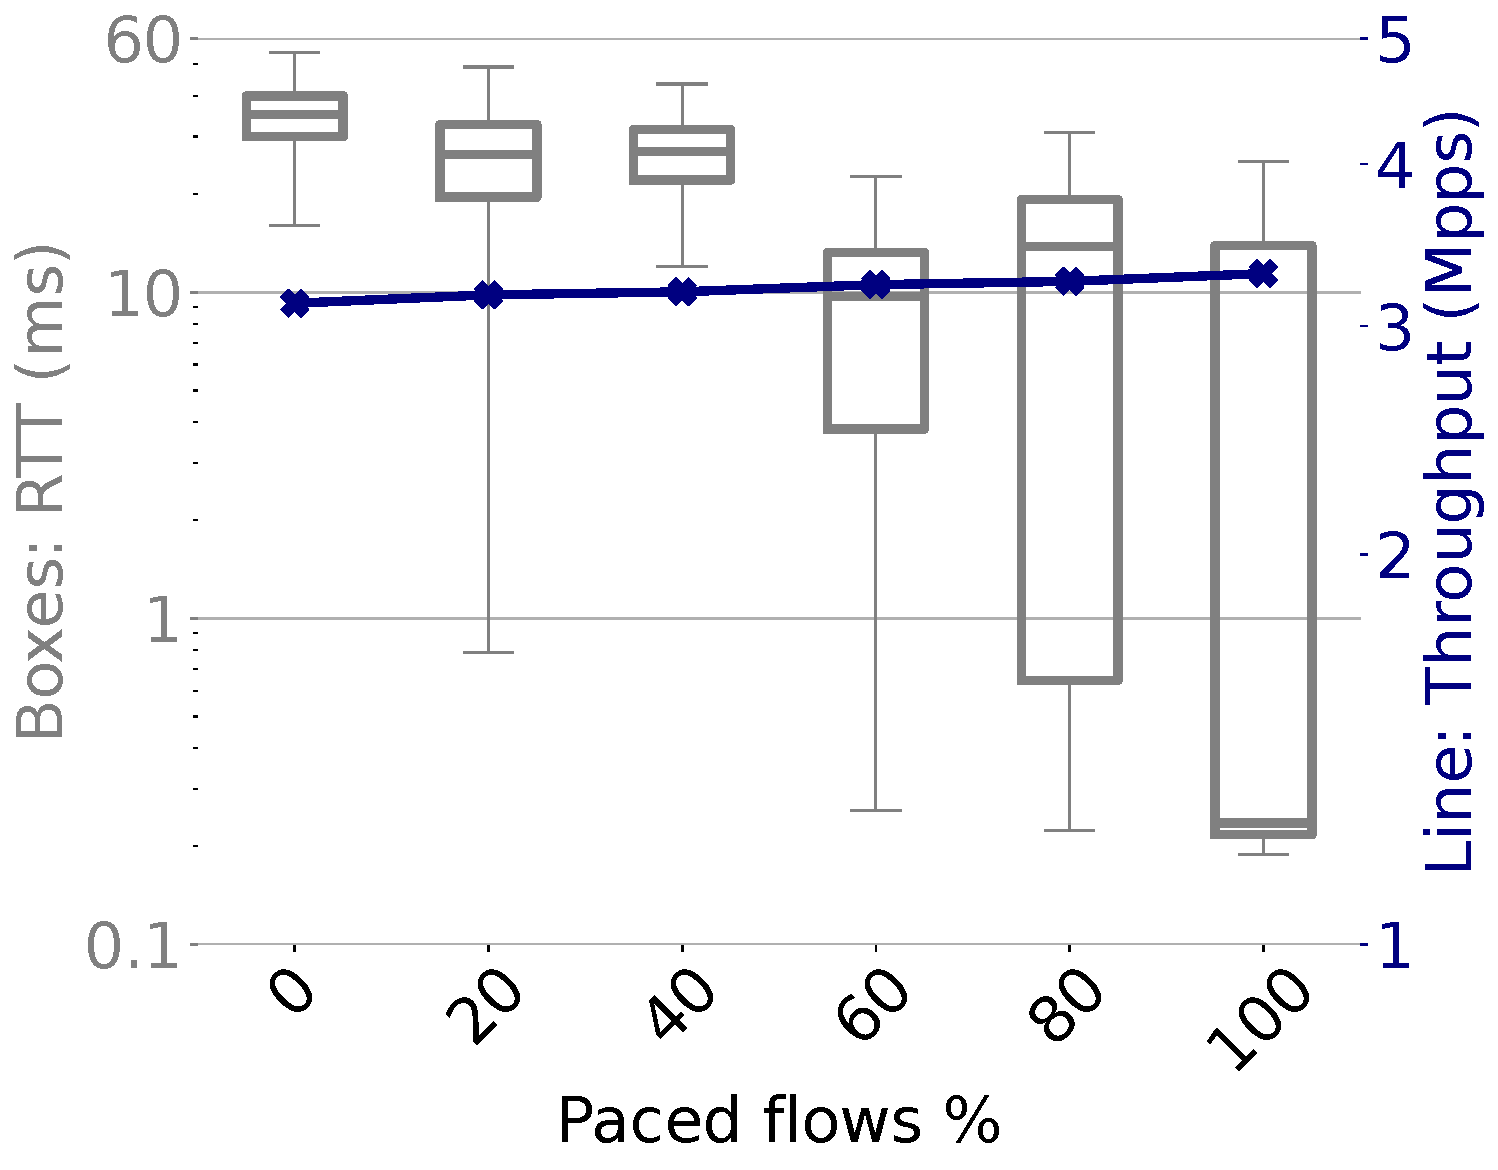
\includegraphics[width=1\linewidth]{figs/pacing_intra_rack_rtt_tput.pdf}
    \caption{Intra-Rack M/R}
	\label{fig:pacing_rack}
\end{subfigure}
\begin{subfigure}[t]{0.40\linewidth}
    \centering
    	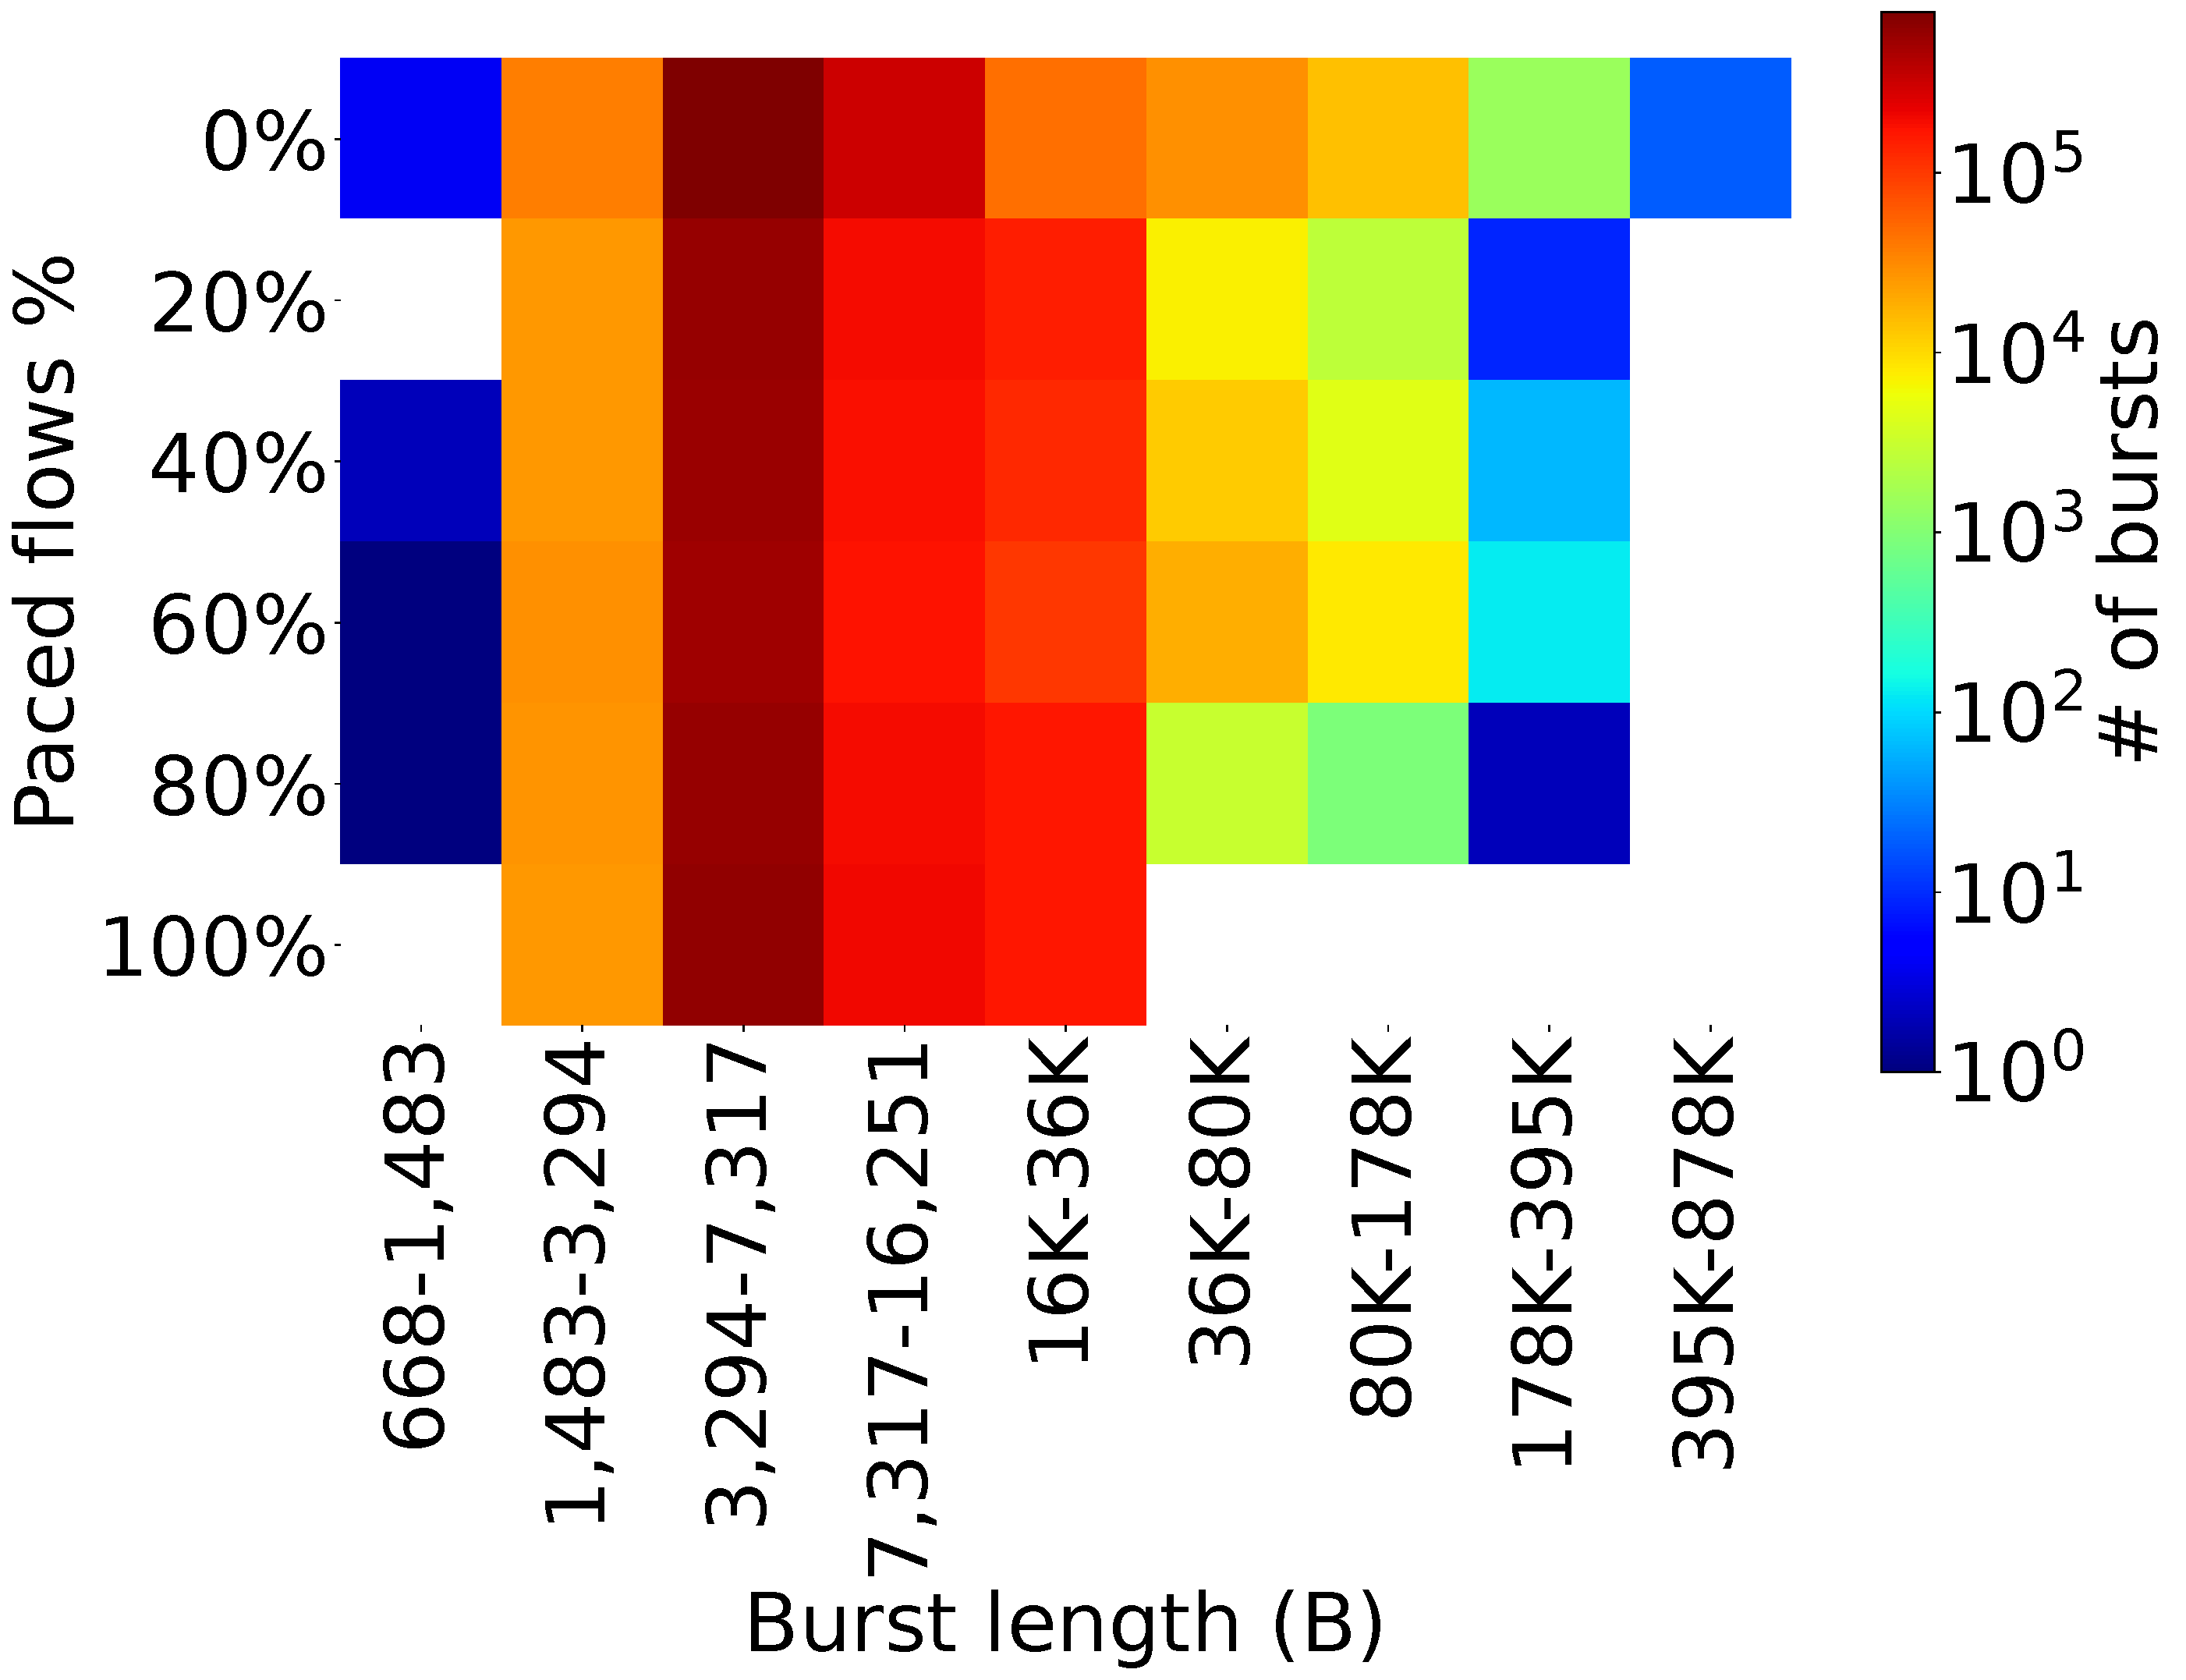
\includegraphics[width=1\linewidth]{figs/pacing2.pdf}
    	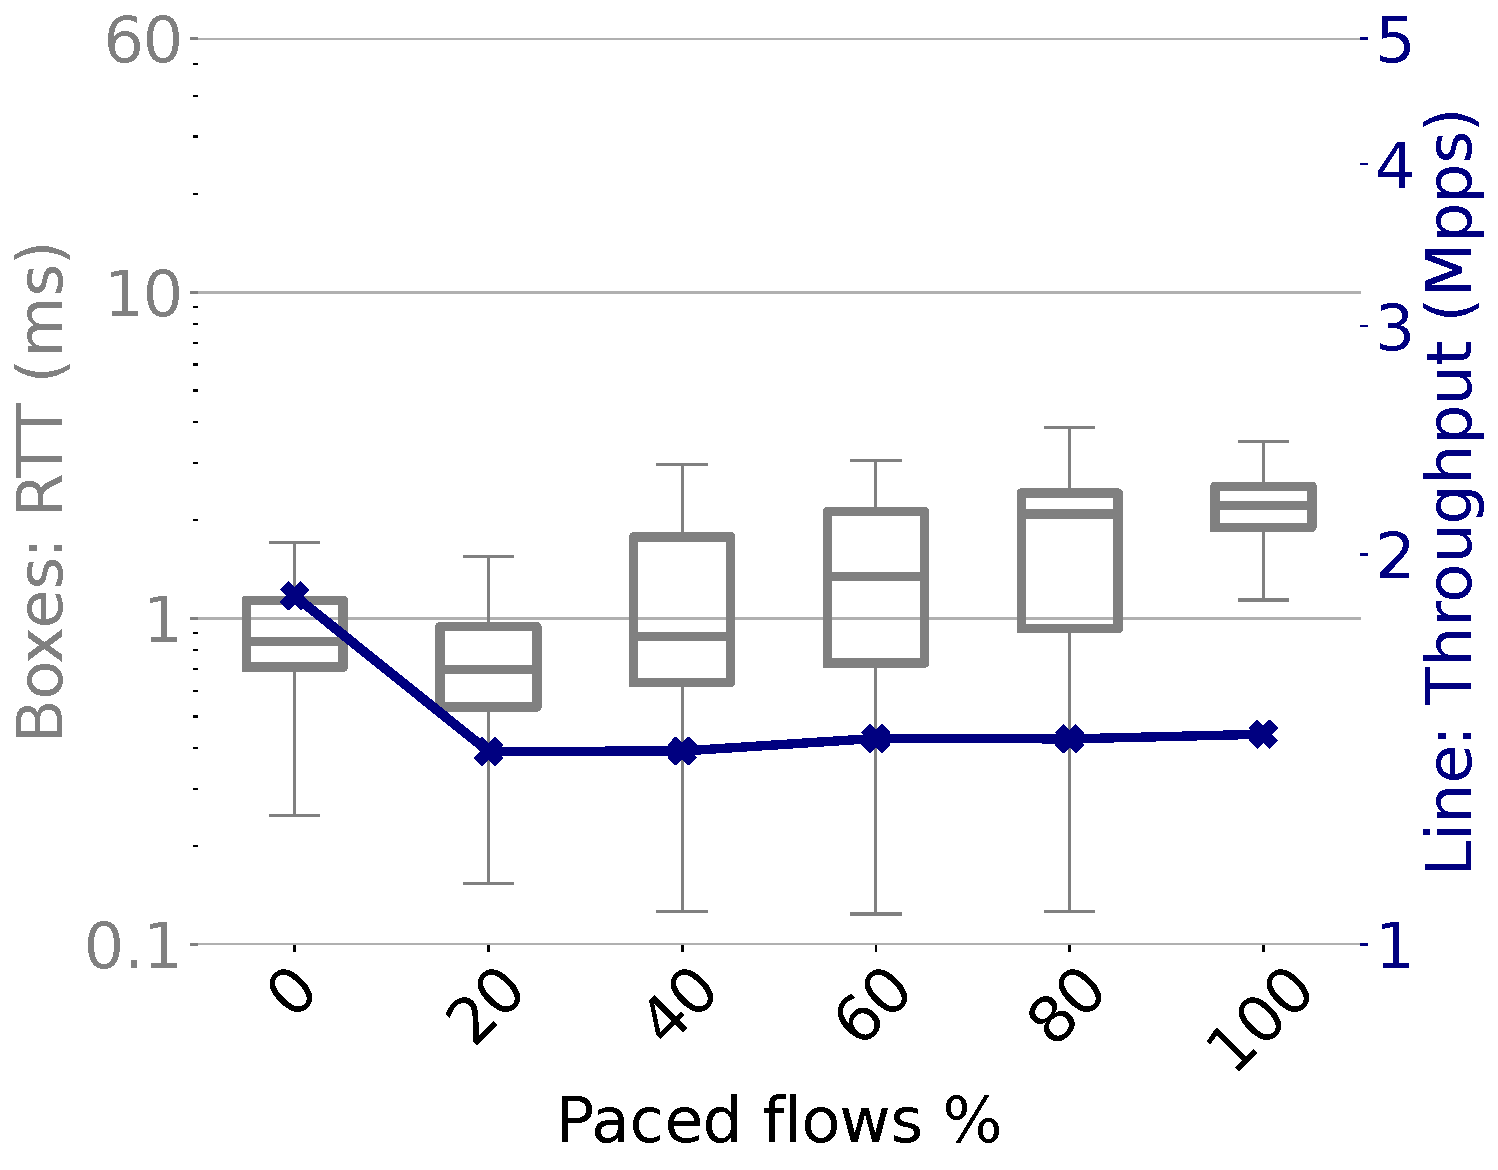
\includegraphics[width=1\linewidth]{figs/pacing_intra_cluster_rtt_tput.pdf}
    \caption{Intra-cluster M/R}
	\label{fig:pacing_cluster}
\end{subfigure}
    	% \vspace{-2mm}
    \caption{\small{Software pacing is workload dependent. For workloads consisting of large flows, its impact on smoothing bursts is unmade by lower layers. For workloads with both short and long flows, it reduces throughput.}}
    \vspace{-2mm}
	\label{fig:pacing}
\end{figure}

\subsubsection{Software pacing}
\label{sec:pacing}
The above observations raise another important question on host networking design decisions. While many congestion control techniques \cite{bbr,homa,swift,outcast,pacing} advocate for pacing in order to achieve accurate control over in-transit data, existing pacing implementation in the Linux kernel is deeply away from the wire, at fq qdisc. \emph{Are qdiscs a suitable place for enforcing pacing?}
To investigate, we repeat the map-reduce (M/R) workloads on the server with both offloading and NIC scheduling enabled and observe that \textit{for workloads with large flows (intra-rack M/R), pacing doesn't have a significant impact on burstiness, and for those with short flows (intra-cluster M/R), pacing results in throughput reduction.} Overall, our results highlight the limitations of software pacing for data center workloads.



Concretely, we configure \textit{fq} to pace 200 flows based on their fair share of bandwidth (200 Mbps), and gradually increase the portion of the flows that are counted as heavy hitters from 0\% (no flow is paced) up to 100\% (all flows are paced).
Figure \ref{fig:pacing} compares the bursts for (a) workload with mostly large flows and (b) workload with a mix of small and large flows. 
In the former workload, we observe that while the impact of pacing ratio is less evident, pacing allows for better bandwidth allocation and the line rate is preserved for all rows. On the other hand, in the latter workload, the throughput is reduced by 22\% under pacing.
This is because short flows are not able to make up for the freed bandwidth that pacing creates.
We also compare packet RTTs and find that pacing large heavy-hitters helps reduce median RTTs by two orders of magnitude as short flows experience less head-of-the-line blocking. This behavior changes in the intra-cluster workload as we do more pacing, as the increased RTT of paced flows drives the overall median RTT up by 160\%.
Further details on the theoretical analysis of burstiness under software pacing can be found in Appendix \S\ref{sec:app-pacing}.


% \subsection{NIC optimizations}
% \begin{figure}[t]
% 	\centering
% 	\begin{subfigure}[t]{.48\linewidth}
% 		\centering\includegraphics[width=1\linewidth]{figs/13_summary_18_0.png}
% 		\caption{Web traffic}
% 		\label{fig:offload1}
% 	\end{subfigure}
% 	\begin{subfigure}[t]{.48\linewidth}
% 		\centering\includegraphics[width=1\linewidth]{figs/14_summary_18_0.png}
% 		\caption{Multi-client Iperf}
% 		\label{fig:offload2}
% 	\end{subfigure}
% 		\begin{subfigure}[t]{.98\linewidth}
% 		\centering\includegraphics[width=1\linewidth]{figs/14-3_summary_14_0.png}
% 		\caption{Single-client Iperf}
% 		\label{fig:offload3}
% 	\end{subfigure}
% % 	\vspace{-1em}
% 	\caption{\small{NIC offloading burstiness study for (a) Web traffic, (b) multi-flow iperf traffic, and (c) single-flow iperf traffic. }} 
% 		\label{fig:offload}
% % 	\vspace{-1em}
% \end{figure}

% \textbf{TCP Segmentation Offload (TSO).} In Linux kernel, packets are represented as arbitrary-sized\footnote{The maximum segment size is set to 64KB.} chunks of memory with a single shared metadata for TCP/IP headers. Since breaking the data into MTU chunks requires multiple memory accesses, allocation and deallocation of packets, and various function calls on smaller data chunks, NIC vendors enable offloading this segmentation to be executed entirely in the hardware, saving a considerable amount of CPU time. This feature is exclusively available for TCP packets properly represented in a kernel sk\_buff data structure.
% \\
% \textbf{Generic Segmentation Offload (GSO).}
% When TSO is not available, kernel can resort to software-based TCP segmentation offload in the driver. While CPU bandwidth is required to perform segmentation, since previous network processing stages are still working on large sk\_buffs, some reduction in CPU utilization is still expected. Both GSO and TSO are anticipated to create longer bursts due to the forced batching they enforce on each flow.
% \\
% \textbf{Scatter/Gather I/O \& Checksum Offload.}
% Scatter/Gather allows the operating system to offload the burden of fetching packet data from various locations in system's memory to the NIC. SG relies on TSO and can further reduce the memory and CPU footprints of packet processing on TX path. 

% In figure \ref{fig:offload} we present the heatmap for number of bursts observed under (a) synthetic web, and (b) concurrent iperf workloads. For a web traffic, since the majority of server responses are short (65\% of the data are <10KB \cite{social}), the offloading features are not put to test. Therefore, disabling offloading has negligible impact on traffic burstiness. However, under a throughput-sensitive workload, we find that TSO creates a large number of 2-packet bursts and considerably fewer number of larger bursts compared to the cases where we disable TSO. That is because, the large segments are passed through to the NIC by the software while the default qdisc in the system, fq,  transmits segments based on a deficit of 2 MSS among flows to enforce fairness (see \ref{sec:qdisc}).

% Due to the impact of packet scheduling for the workload under study, we repeat the iperf tests, limiting the number of concurrent iperf connections to one. Figure \ref{fig:offload3} demonstrates that disabling scatter/gather forces the software stack to perform serialization on the data, significantly blunting the impact of $\mu$bursts.

% \begin{tcolorbox}
% \textbf{Finding x}

% Packet data serialization performed by scatter/gather can significantly reduce the burstiness.

% Under multi-flow scenario, TSO breaks longer bursts into small 2-packet $\mu$bursts for throughput-sensitive workloads. Additionally, TSO is prone to  creating very longer bursts.
% \end{tcolorbox}


\subsubsection{Byte Queue Limits}
% \begin{figure}[t]
% 	\centering
% 	\begin{subfigure}[t]{.45\linewidth}
% 		\centering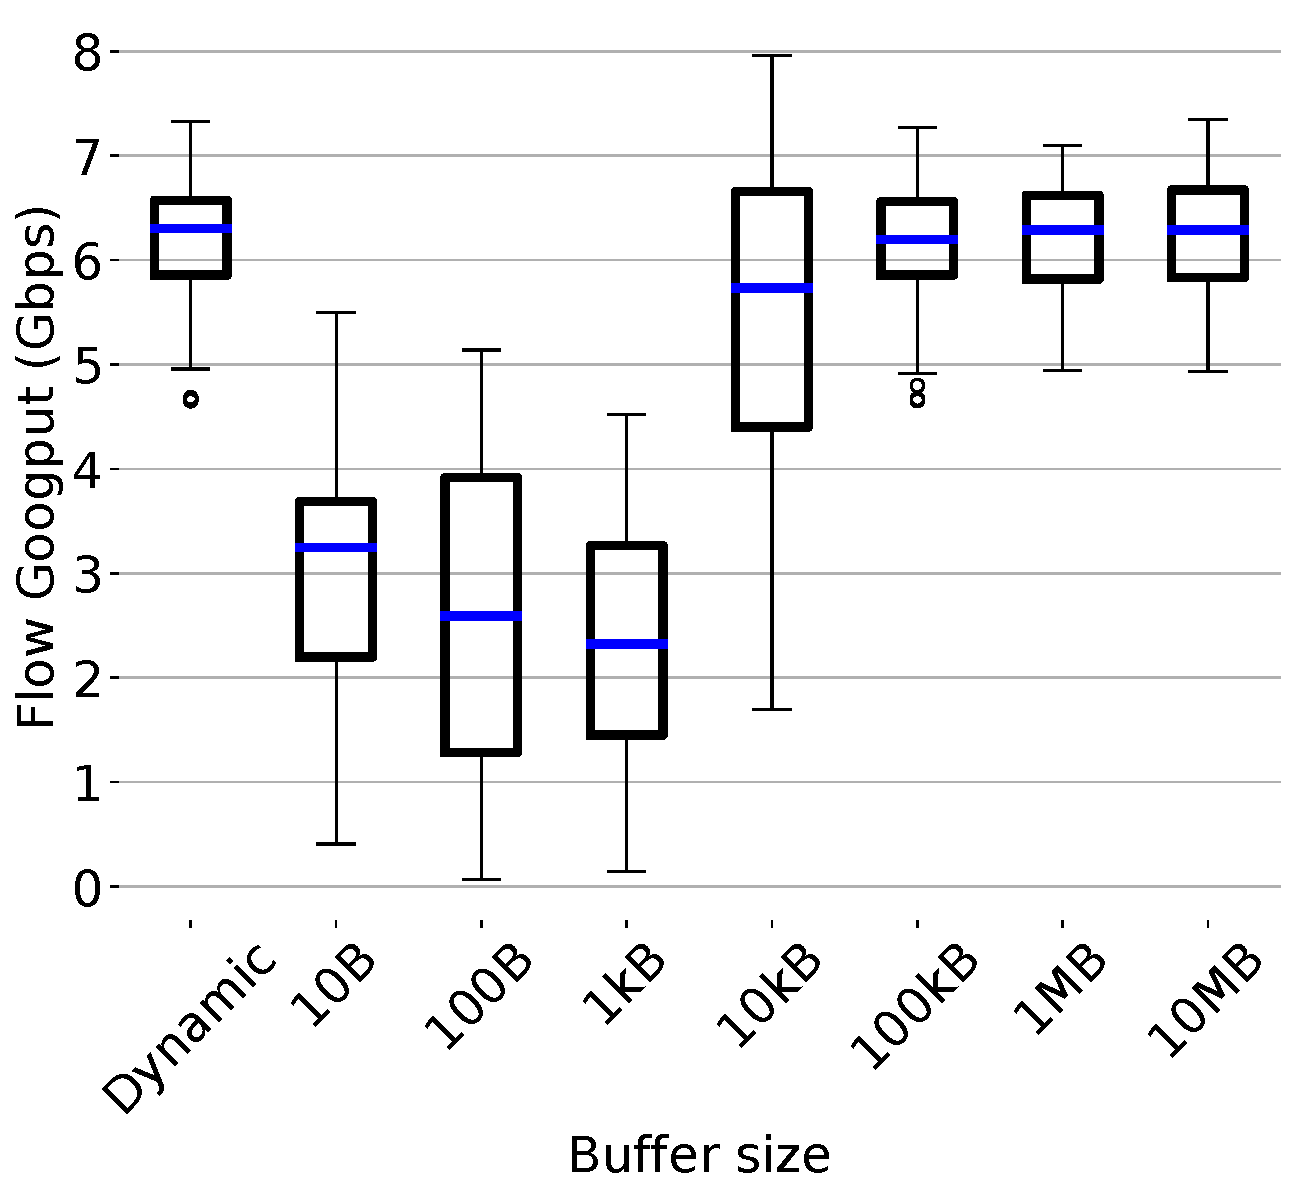
\includegraphics[width=1\linewidth]{figs/tso_gput.pdf}
% 		\caption{IPerf flow goodput}
% 		\label{fig:offload_latency1}
% 	\end{subfigure}
% 	\begin{subfigure}[t]{.45\linewidth}
% 		\centering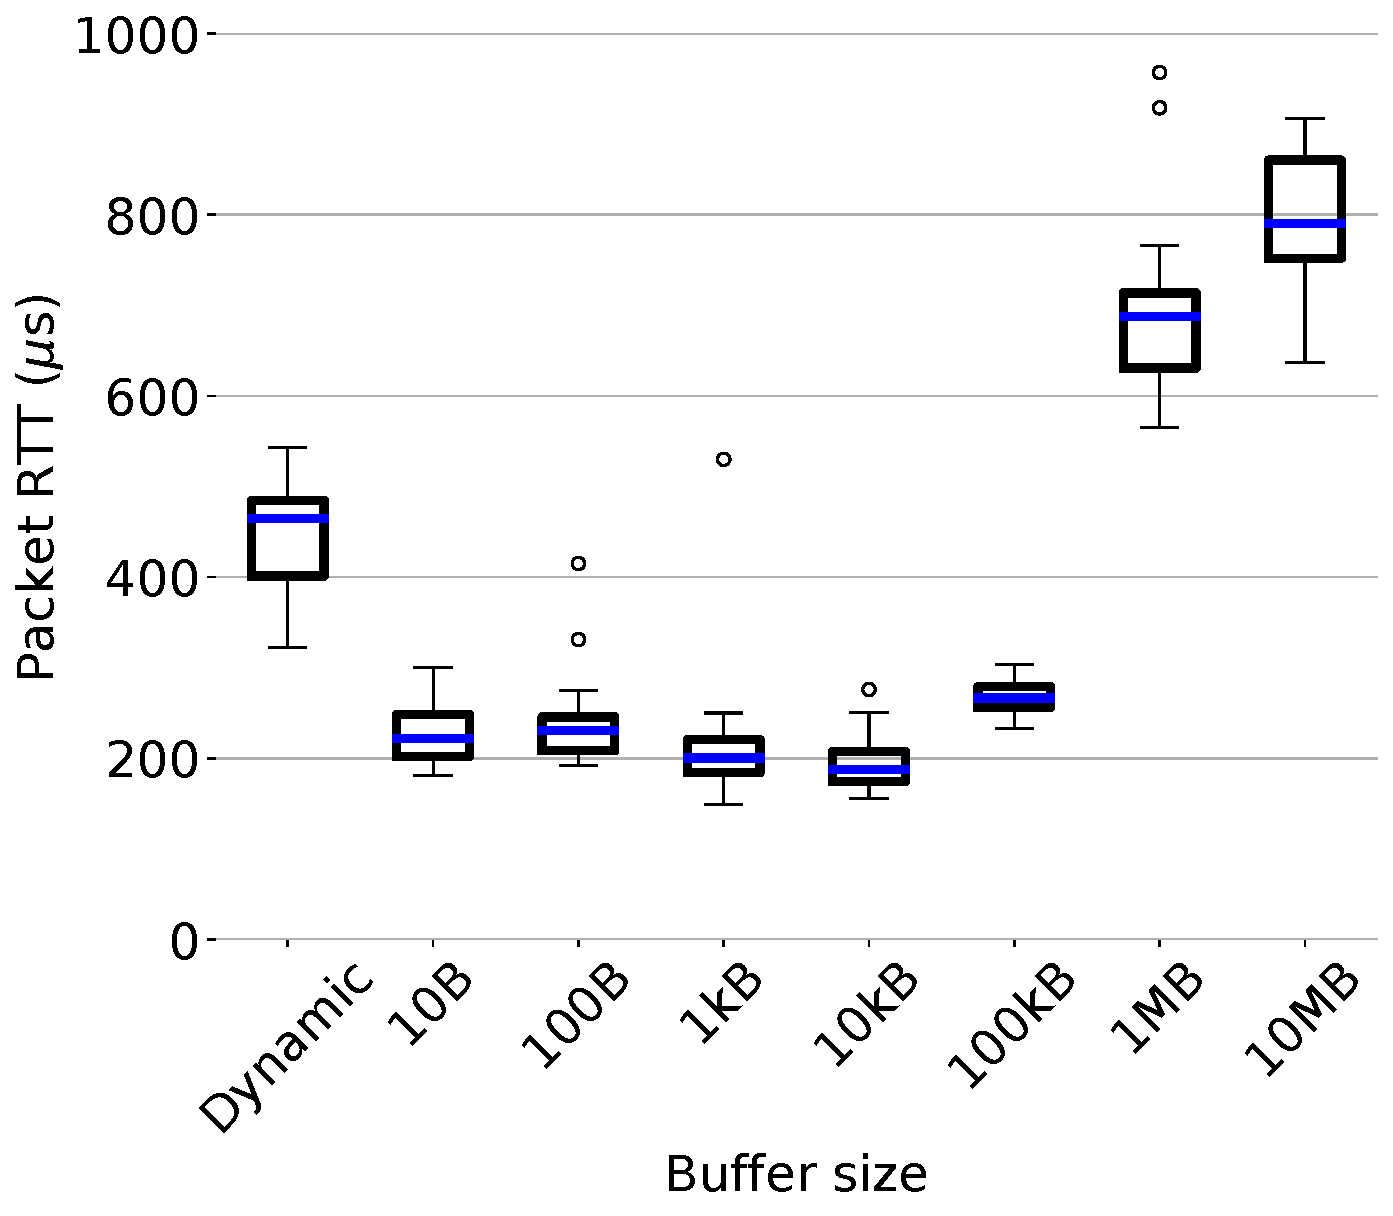
\includegraphics[width=1\linewidth]{figs/tso_rtt.pdf}
% 		\caption{Iperf RTTs}
% 		\label{fig:offload_latency2}
% 	\end{subfigure}
% 	\vspace{-4mm}
% 	\caption{\small{Larger driver rings produce a higher throughput at the expense of higher packet RTTs.}} 
% 		\label{fig:bql_latency}
% 		\vspace{-4mm}
% \end{figure}
\begin{figure}[t]
	\centering
 	\begin{subfigure}[t]{.26\linewidth}
	\centering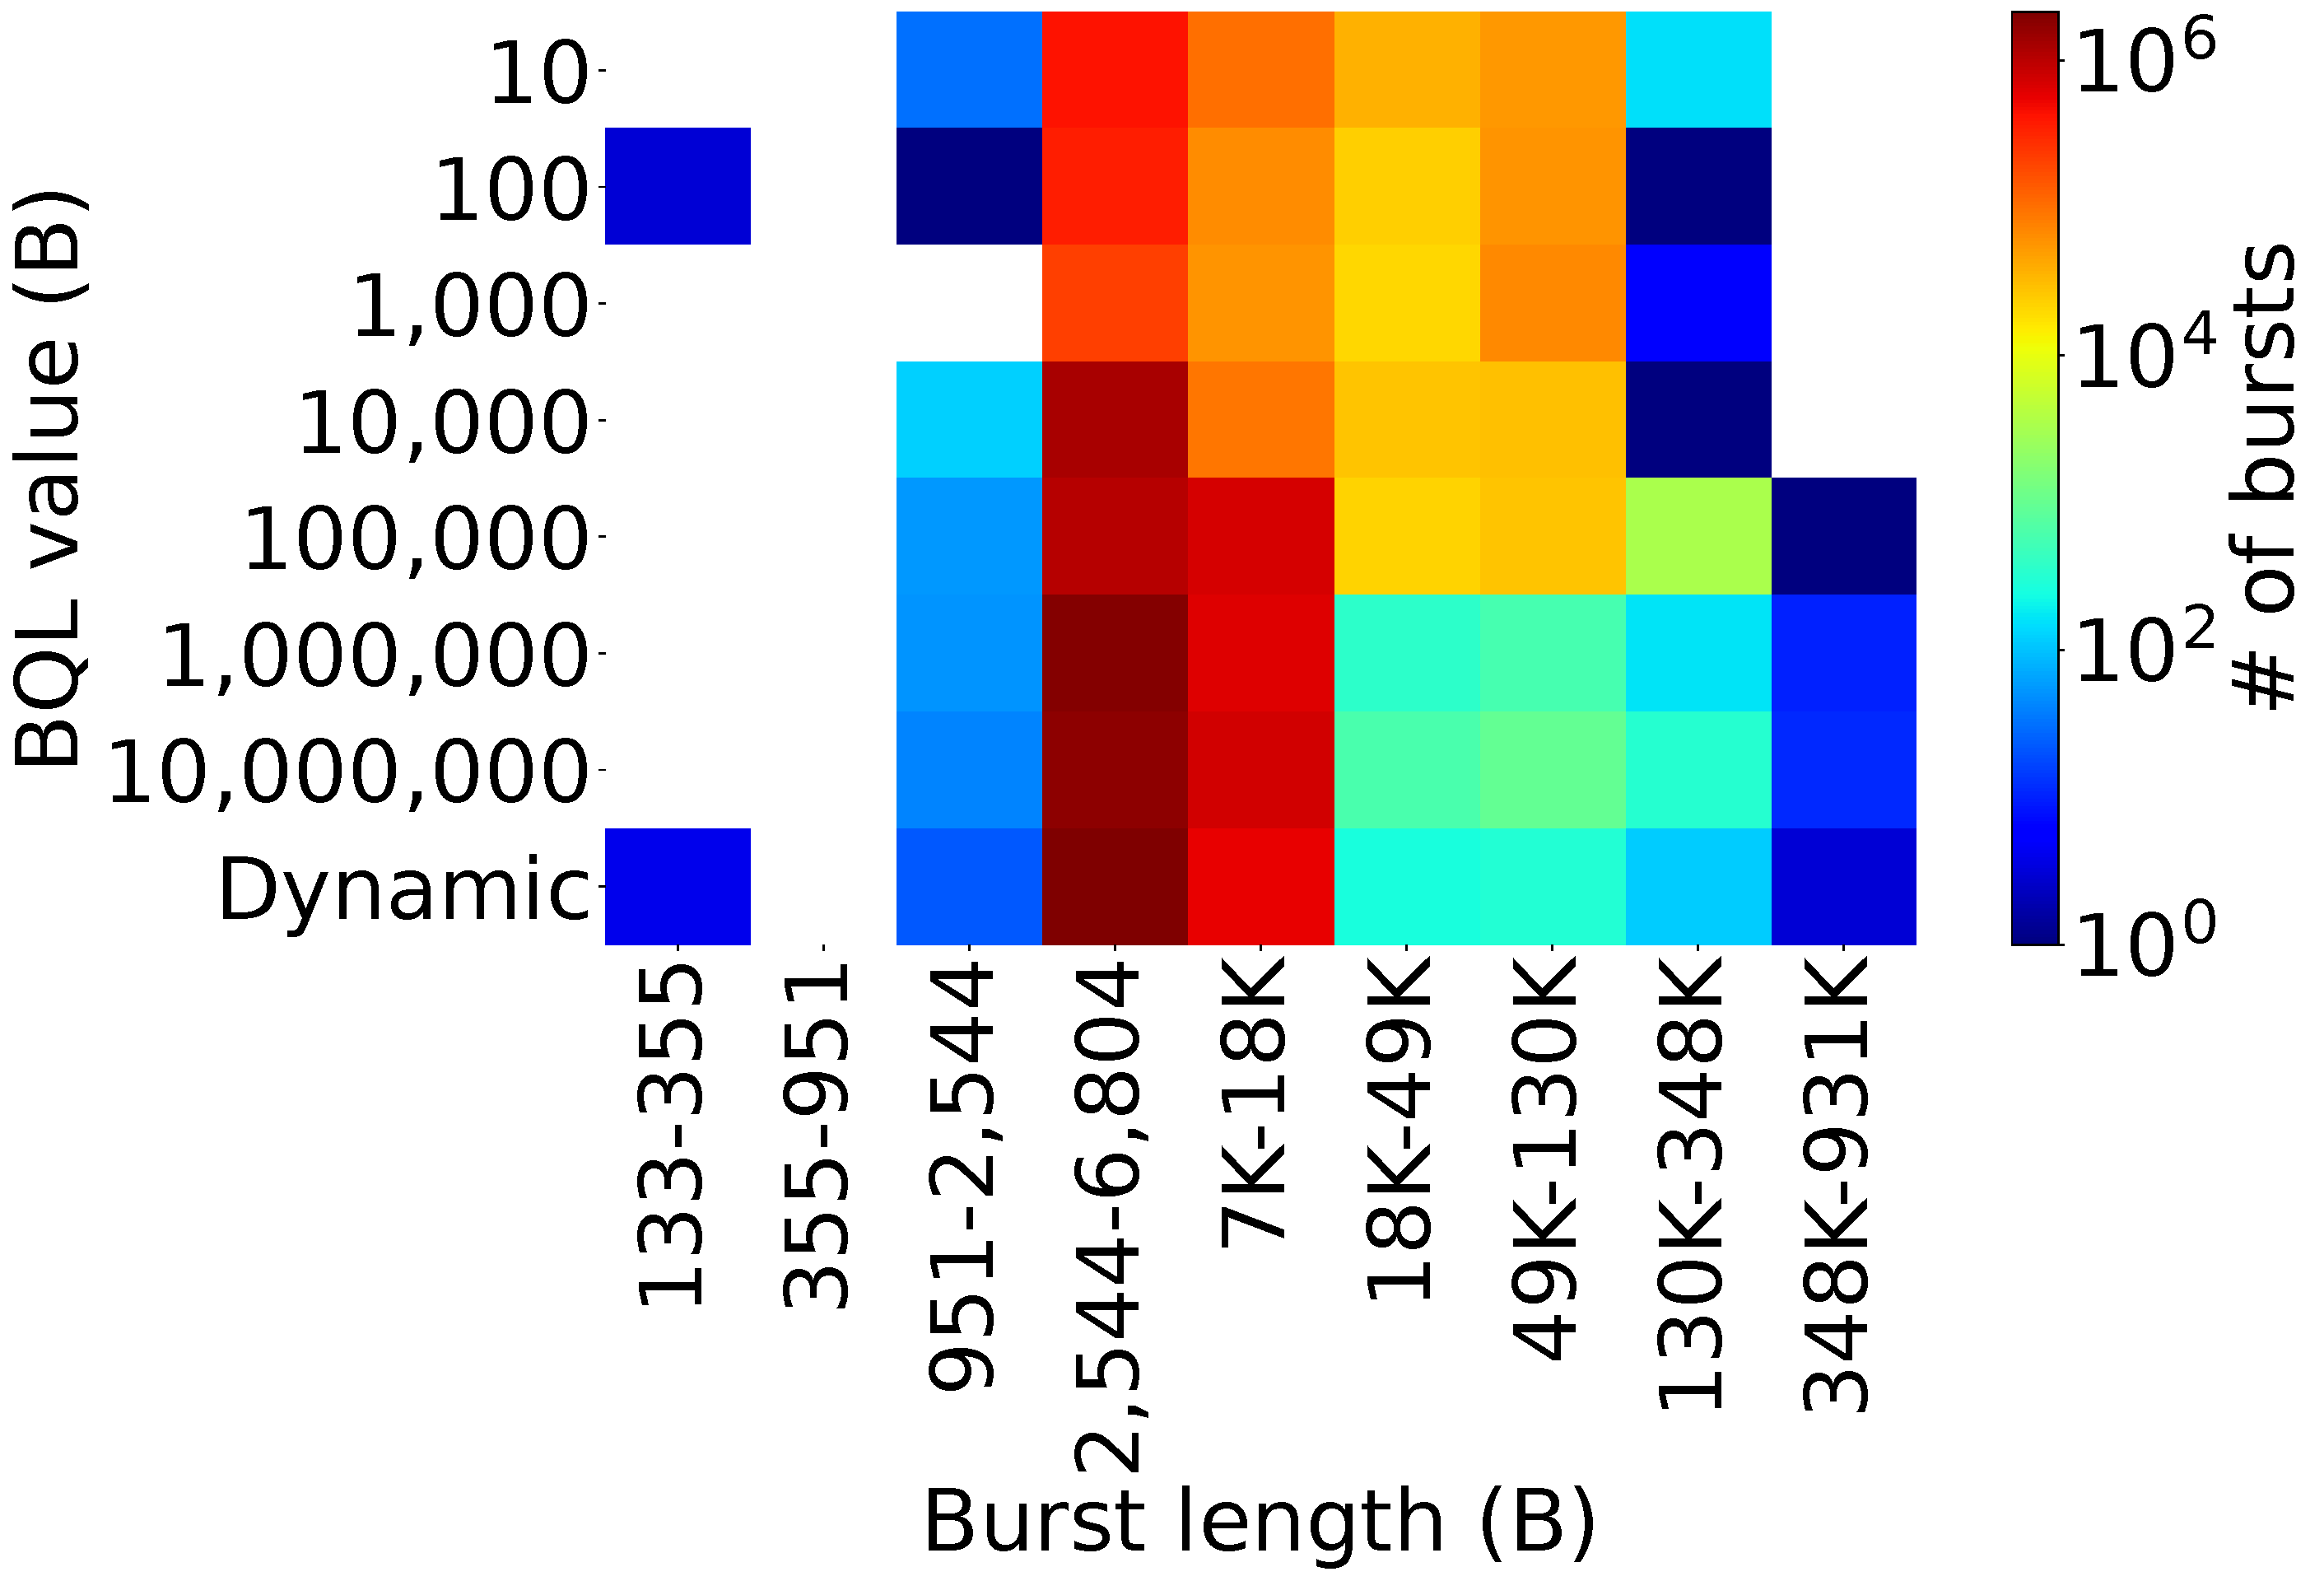
\includegraphics[width=1\linewidth]{figs/bql1.pdf}
			\vspace{-2mm}
	\caption{Burst heatmap}
    \label{fig:bql}
    \end{subfigure}
	\begin{subfigure}[t]{.26\linewidth}
	\centering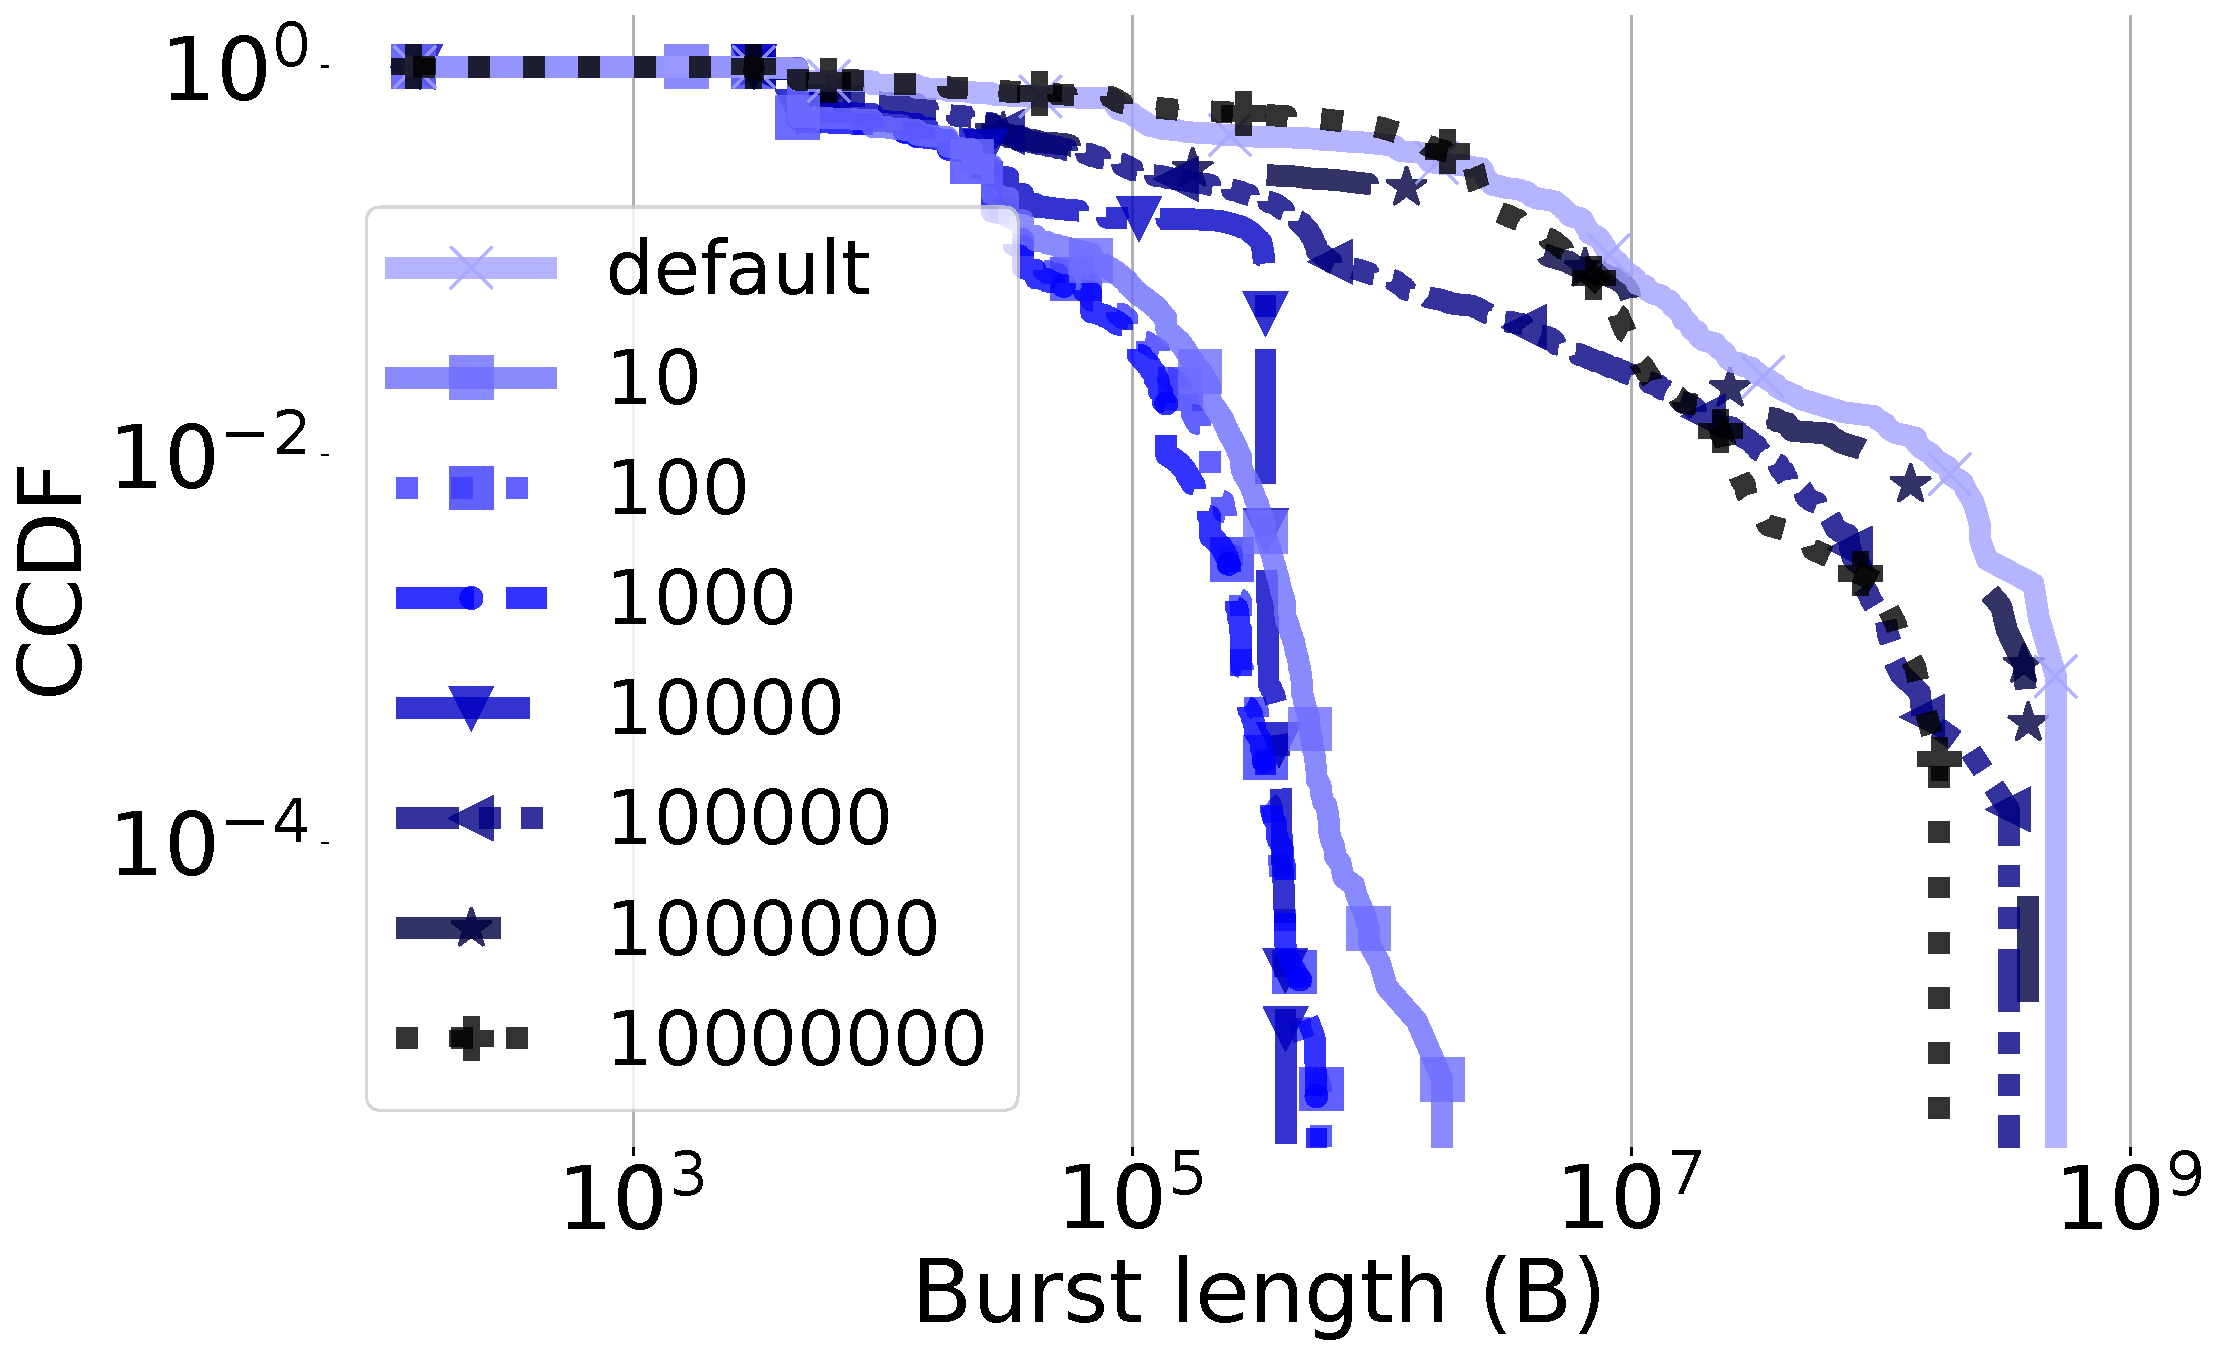
\includegraphics[width=1\linewidth]{figs/bqlccdf_testbed.pdf}
			\vspace{-2mm}
	\caption{Microburst CCDF}
    \label{fig:bql-ccdf}
    \end{subfigure}
    	\begin{subfigure}[t]{.22\linewidth}
		\centering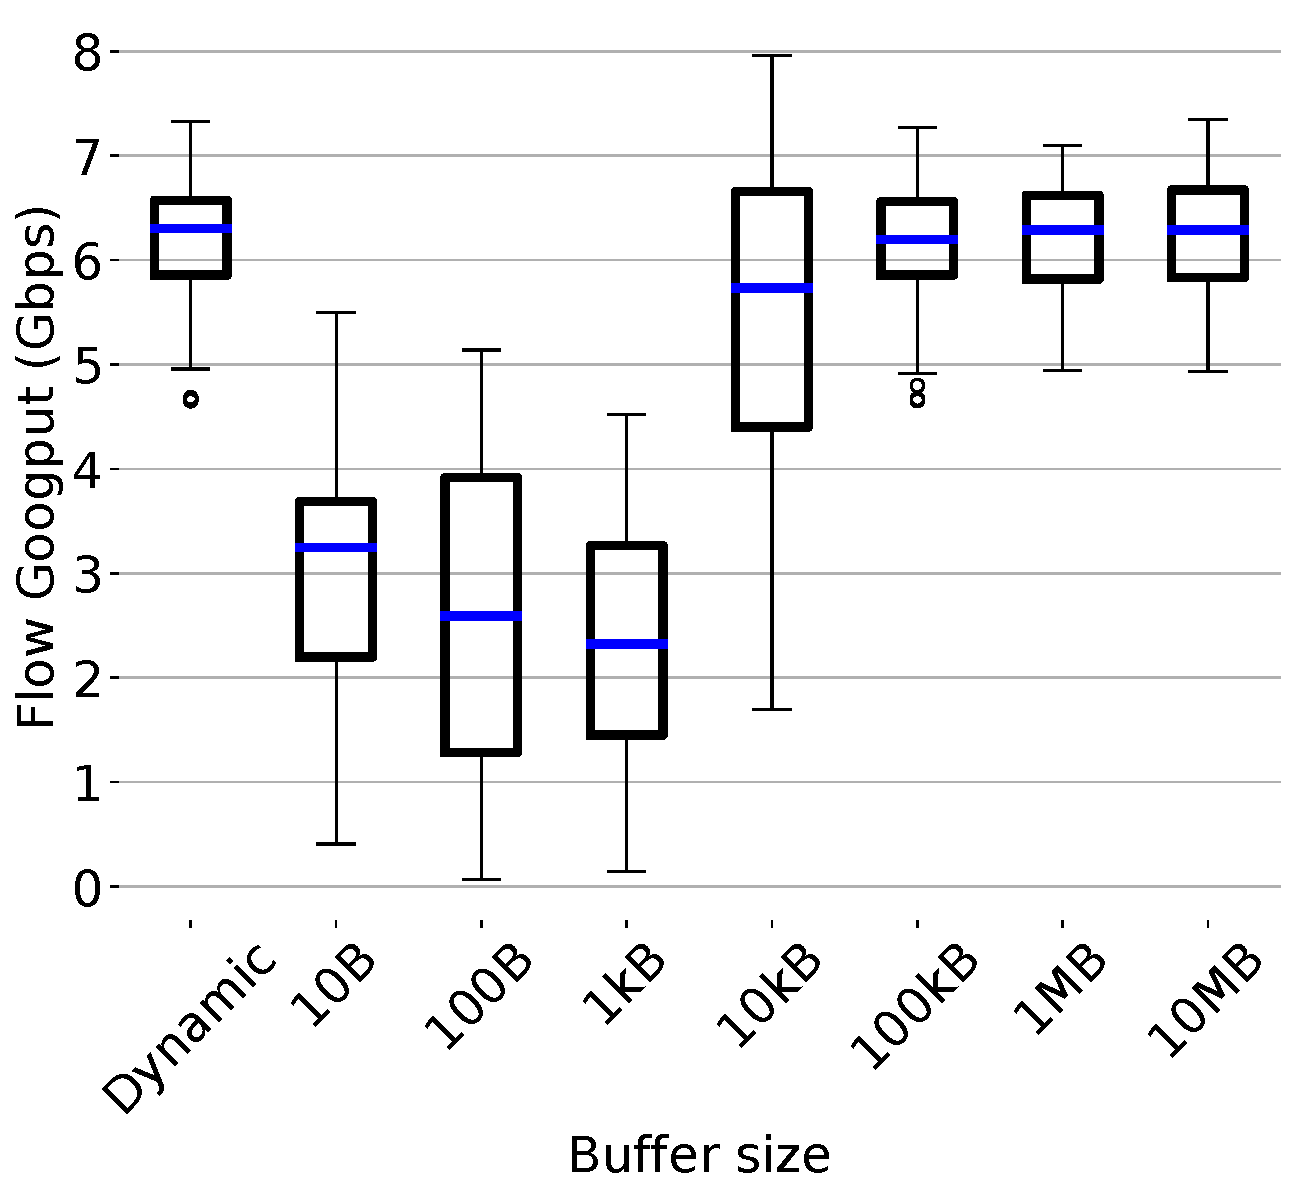
\includegraphics[width=1\linewidth]{figs/tso_gput.pdf}
        \vspace{-2mm}
		\caption{Flow goodput}
		\label{fig:offload_latency1}
	\end{subfigure}
	\begin{subfigure}[t]{.22\linewidth}
		\centering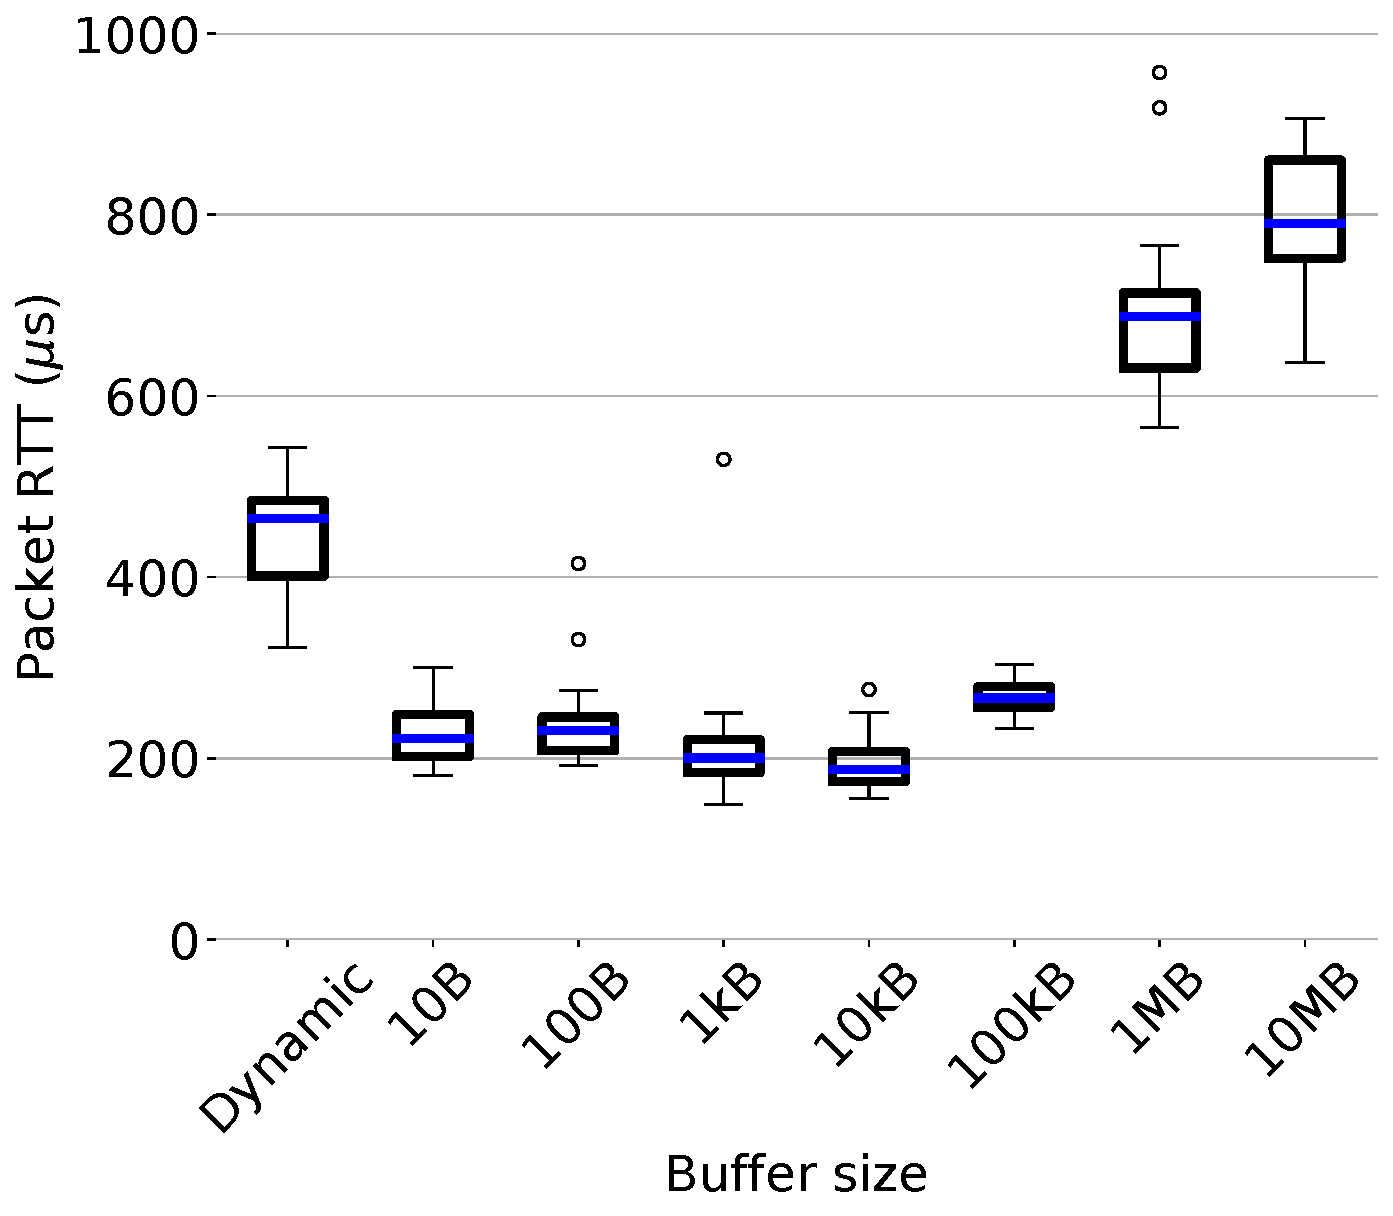
\includegraphics[width=1\linewidth]{figs/tso_rtt.pdf}
        \vspace{-2mm}
		\caption{Packet RTTs}
		\label{fig:offload_latency2}
	\end{subfigure}
% \vspace{-2mm}
	\caption{\small{Larger BQL settings produce longer bursts. Also, the dynamic BQL algorithm presents a similar behavior to a large static ring size.}}
		\label{fig:bql_all}
% 	\vspace{-1em}
\vspace{-2mm}
\end{figure}

Linux kernel employs buffers at various stages of network stack processing to streamline the data movement among various components. The NIC driver queue is the last buffering stage before triggering the hardware. A fixed-size driver queue (a.k.a., TX ring) would ensure that the NIC can always find ready-to-send packets without communicating with the OS. However, due to the unpredictable size of packet buffers in the Linux kernel (ranging from 64B up to tens of kilobytes), the queueing time will considerably add to the overall RTT of packets. To prevent that, OS developers propose a dynamic bound on TX rings that adjusts the limit based on NIC's transmission rate and the availability of data in the TX rings \cite{bql}. To that end, after every transmission, BQL uses time intervals to check whether the NIC was starved in previous transmissions. If the NIC was not fully utilized during any interval while data was available at higher layers, the BQL algorithm increases the limit on the TX ring. Otherwise, if the NIC was fully busy, the BQL is decreased to reduce the queueing overheads. Enforcing smaller queue limits also ensures that the main queuing occurs at the qdisc-level where more advanced queuing disciplines can be employed.

Apart from Linux, NIC buffer sizing is also an important consideration for kernel-bypass runtimes that are less inclined to distribute TX processing among multiple ring buffers \cite{shenango,tas}. Figure \ref{fig:bql_all} demonstrates the impact of driver queue size on performance and burstiness. Intuitively, as we increase the size of the driver's buffer, we greatly increase the queueing time experienced by egress traffic, therefore, preventing the bursts of packets from arriving at the NIC. On the other hand, a larger driver queue is more prone to creating longer bursts as it is more susceptible to triggering segmentation offload (99$^{th}$ percentile burst length for 1 KB buffers and 1 MB buffers are 68 KB and 9 KB, respectively, but 99.99$^{th}$ lengths shift to 68 KB and 86 KB, respectively). The microburst length distributions in Figure \ref{fig:bql-ccdf} further suggest that the default dynamic buffer sizing algorithm tends to maintain larger ring buffers which leads to longer bursts.


\subsubsection{Linux process scheduling}
Apart from the network stack, the operating system features various internal components that might change the traffic shape. For example, Linux offers a range of process scheduling classes suited for various use cases:
\\
\textbf{Completely Fair Scheduler (CFS)} is the default process scheduling class in Linux which aims at achieving fairness among active processes in the system while maintaining responsiveness for I/O-bound applications. when running a mix of compute-intensive and network-intensive workloads, CFS attempts to proportionally share the CPU among workloads leading to longer response times \cite{tales}.
\\
\textbf{Real-time scheduler} supports two policies: \textit{Round-robin} and \textit{First-In-First-Out (FIFO)} scheduling. Both policies give strict priority to I/O-bound applications (if configured properly). By default, the round-robin policy preempts high-priority processes every 100ms while the FIFO policy is non-preemptive. We also deploy Microquanta \cite{snap,microquanta} a semi-real-time scheduling class with microsecond time precision.
% \textbf{Microquanta scheduler} is a more recent attempt at introducing process schedulers with microsecond time precision. Microquanta was introduced as part of Snap microkernel \cite{snap} to allow fine-grained time accounting among userspace processes as well as among real-time and non-real-time applications. We deploy a publicly available implementation of Microquanta on our testbed and configure it to switch between available processes in 50$\mu$s intervals. We also adjust the CPU time allocation between background and network apps to 4-1. This means that Microquanta will allocate 80\% of its time window to the higher-priority network processes.
\begin{figure}[t]
\centering
% \begin{subfigure}[t]{0.8\linewidth}
%     \centering
%     	\includegraphics[width=1\linewidth]{figs/sched_hurst.pdf}
%          \caption{\small{\textbf{Hurst estimates for different process schedulers}}}
% 	\label{fig:sched-hurst}
% \end{subfigure}
\begin{subfigure}[t]{0.90\linewidth}
    \centering
    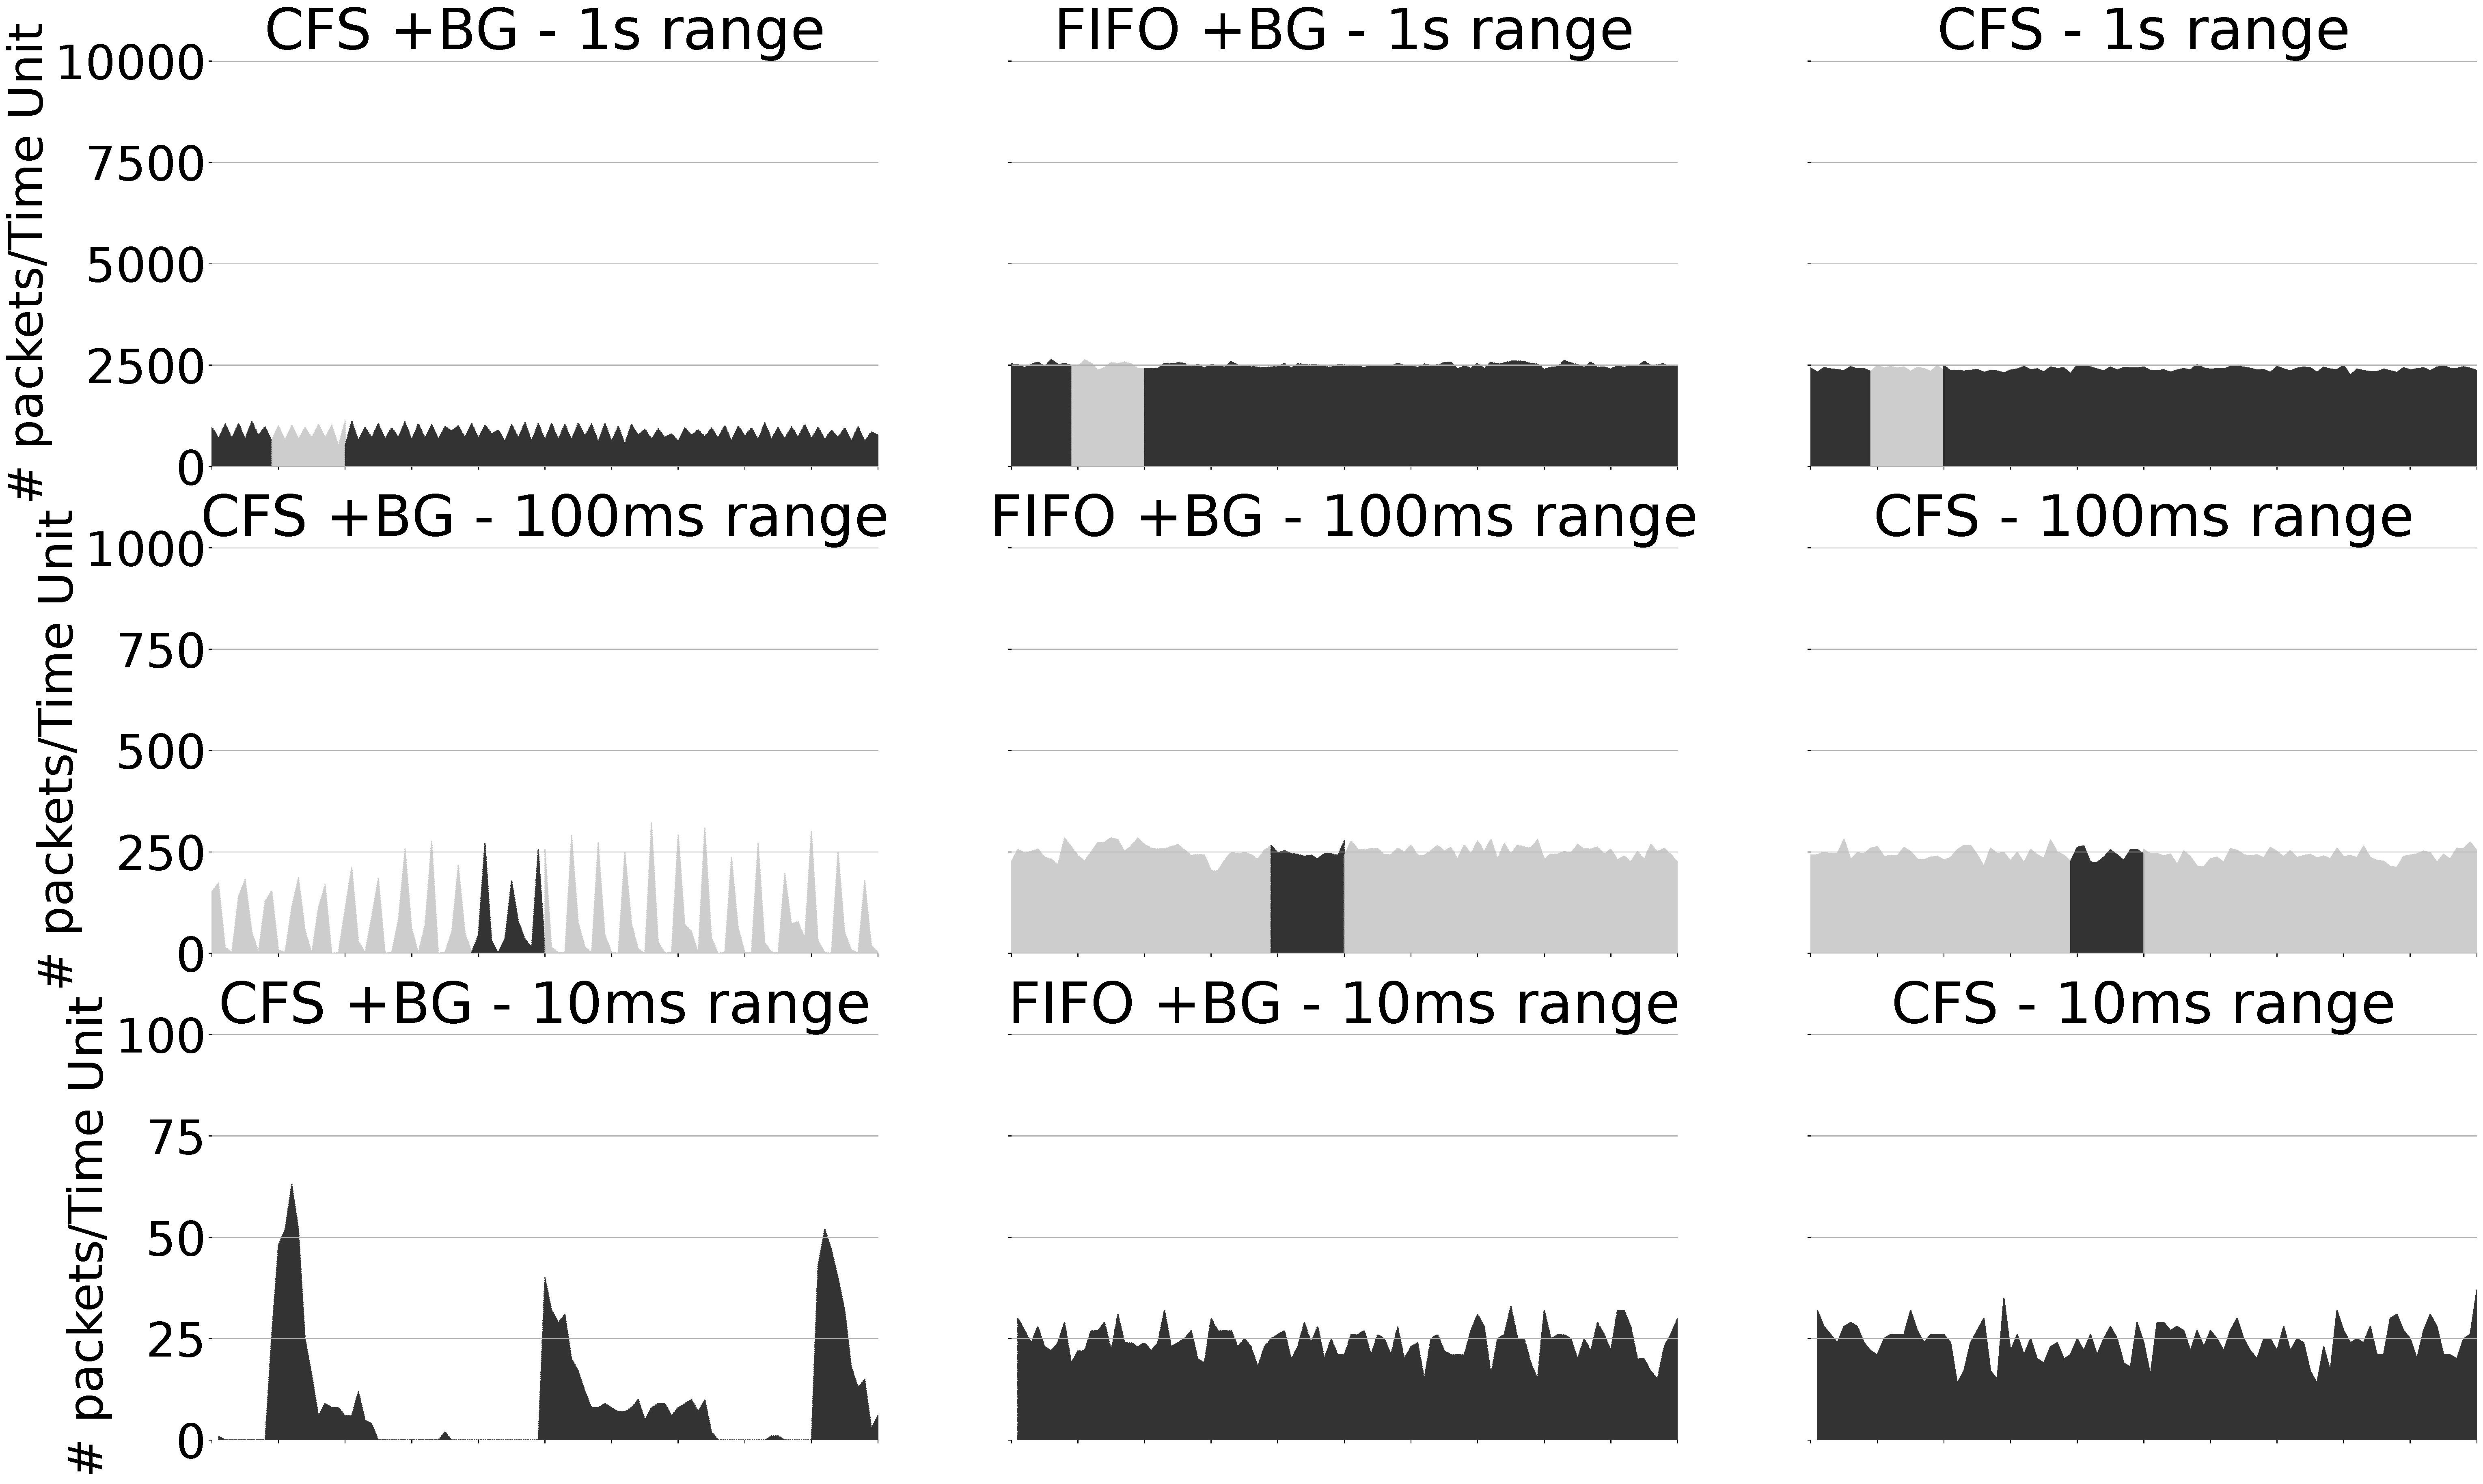
\includegraphics[width=1\linewidth]{figs/sched_ts.pdf}
 %    \caption{\small{\textbf{Timeseries of packet arrivals}}}
	% \label{fig:sched-ts}
\end{subfigure}
\vspace{-1mm}
    \caption{\small{Impact of process scheduling on traffic bursts.}}
	\label{fig:sched}
 \vspace{-2mm}
\end{figure}

Valinor's picture of traffic burstiness is consistently similar when  the network application is running alone as Hurst estimates vary between 0.51 and 0.54 for all the schedulers. However, when the background process is introduced, a course-grained process scheduler like CFS must enforce fair CPU time sharing, resulting in the leap of its H estimate to 0.74 while other schedulers are able to schedule the network application's threads in short timescales and result in smooth transmissions. To validate the self-similarity estimates, we plot the time series of CFS (running only the network workload), CFS+BG (running the network workload alongside background threads), and the real-time FIFO scheduler running both applications (FIFO+BG) in Figure \ref{fig:sched}. The self-similar nature of the CFS+BG scenario is noticeable in the leftmost column as CFS causes the network packets to be sent in larger chunks, causing intermittent but larger bursts at short time spans.

\section{Conclusions}
\label{sec:valinor-conclusion}

We presented the design of Valinor, a burst measurement framework that consists of an in-host eBPF framework and an in-network timestamping module for programmable switches. Valinor can capture burstiness at different scales (ranging from nanoseconds to seconds).
We use Valinor to demonstrate how host networking elements affect bursts. 
We show that the scaling behavior of traffic at long timescales and burstiness at fine timescales vary significantly across different host networking configurations (process schedulers, congestion control algorithms, single vs. multi-queue NICs, etc.) and across different classes of practical workloads. In particular, we show the impact of hardware-resident functions (e.g., NIC schedulers) that are largely overlooked in characterizing burstiness. 
%Leveraging this ability, we use theoretical models of burstiness, like rescaled-range analysis, to show the impact of NIC scheduling, TCP segmentation offload, transport protocols, and process scheduling on burstiness. 
This variability of burstiness and the implications of bursts on performance underscore the need for  measurement systems to perform periodic burst analysis.